% !TEX TS-program = xelatex
% !TEX encoding = UTF-8
\documentclass{article}
\usepackage{kmreport}
%\usepackage{pslatex}
\usepackage{graphicx}
\usepackage[toc,page]{appendix}
\usepackage[framed,numbered,autolinebreaks,useliterate]{mcode}
\input{listingstyle}
\renewcommand*{\lstlistingname}{Code [\textsc{\scriptsize{MATLAB}}]}
\usepackage{mathptmx}	% Use the Postscript Times font
\usepackage[FIGBOTCAP,normal,bf,tight]{subfigure}
\usepackage[normal,bf,tight]{subfigure}
\usepackage[dvips,light,first,bottomafter]{draftcopy}
\draftcopyName{Sample, contains no OUO}{70}
\usepackage{amsmath,amssymb,amsthm,varwidth,array,ragged2e}
\usepackage{wrapfig}
\usepackage{kotex}
\usepackage{multirow}
\usepackage{multicol}
\newcolumntype{L}{>{\varwidth[c]{\linewidth}}l<{\endvarwidth}}
\newcolumntype{M}{>{$}l<{$}}
%\def\ds{\mathrm{d}s}%  don't know what your \ds should be ....
\usepackage[pdfborder={0 0 0}]{hyperref}
\usepackage{algorithm}
\usepackage{algpseudocode}
\numberwithin{equation}{section}
\numberwithin{figure}{section}
\numberwithin{algorithm}{section}
\hypersetup{pdfborder=0 0 0}
%\usepackage{flafter}
%\usepackage[section]{placeins}
\newtheorem{law}{정리}
\newtheorem{theorem}{Theorem}[section]
\newtheorem{lemma}[theorem]{Lemma}
\newtheorem{proposition}[theorem]{Proposition}
\newtheorem{corollary}[theorem]{Corollary}
\newenvironment{proof1}[1][Proof]{\begin{trivlist}
\item[\hskip \labelsep {\bfseries #1}]}{\end{trivlist}}
\newenvironment{definition}[1][Definition]{\begin{trivlist}
\item[\hskip \labelsep {\bfseries #1}]}{\end{trivlist}}
\newenvironment{example}[1][Example]{\begin{trivlist}
\item[\hskip \labelsep {\bfseries #1}]}{\end{trivlist}}
\newenvironment{remark}[1][Remark]{\begin{trivlist}
\item[\hskip \labelsep {\bfseries #1}]}{\end{trivlist}}

\newcommand{\qedd}{\nobreak \ifvmode \relax \else
      \ifdim\lastskip<1.5em \hskip-\lastskip
      \hskip1.5em plus0em minus0.5em \fi \nobreak
      \vrule height0.75em width0.5em depth0.25em\fi}
\theoremstyle{examplestyle}
\newcommand{\paih}[1]{%
\index{packages!#1@\textsf{#1}}%
\index{#1@\textsf{#1}}}
\newcommand{\pai}[1]{%
\paih{#1}\textsf{#1}}
\usepackage{array}
\makeatletter
\newcolumntype{e}[1]{%--- Enumerated cells ---
   >{\minipage[t]{\linewidth}%
     \NoHyper%                Hyperref adds a vertical space
     \let\\\tabularnewline
     \enumerate
        \addtolength{\rightskip}{0pt plus 50pt}% for raggedright
        \setlength{\itemsep}{-\parsep}}%
   p{#1}%
   <{\@finalstrut\@arstrutbox\endenumerate
     \endNoHyper
     \endminipage}}

\newcolumntype{i}[1]{%--- Itemized cells ---
   >{\minipage[t]{\linewidth}%
        \let\\\tabularnewline
        \itemize
           \addtolength{\rightskip}{0pt plus 50pt}%
           \setlength{\itemsep}{-\parsep}}%
   p{#1}%
   <{\@finalstrut\@arstrutbox\enditemize\endminipage}}

\AtBeginDocument{%
    \@ifpackageloaded{hyperref}{}%
        {\let\NoHyper\relax\let\endNoHyper\relax}}
\makeatother
\setmainfont[
    Ligatures=TeX,
    Extension=.otf,
    UprightFont= *-regular,
    BoldFont=*-bold,
    ItalicFont=*-italic,
    BoldItalicFont=*-bolditalic
]{texgyreschola}
%\setmainfont[Mapping=tex-text]{TeX Gyre Pagella}
%\setsansfont[Mapping=tex-text]{Helvetica}
\setmainhangulfont[BoldFont=렉시새봄R,ItalicFont=렉시새봄R,
    ItalicFeatures={FakeSlant=.167}]{렉시새봄R}
%\setmainhangulfont[BoldFont=나눔명조 ExtraBold,ItalicFont=나눔명조,     ItalicFeatures={FakeSlant=.167}]{나눔명조}
\setsanshangulfont[BoldFont=나눔고딕 ExtraBold,ItalicFont=나눔고딕,
    ItalicFeatures={FakeSlant=.167}]{나눔고딕}
%\setmainhanjafont{네이버사전}
\makeatletter
\renewcommand{\tableofcontents}[1][\contentsname]{%
  \section*{#1}
  \begin{multicols}{2}
    \@starttoc{toc}
  \end{multicols}
}
\makeatother

\title{공학 수치해석\\Numerical Analysis for Engineers}
\author{
%Eunchurn Park
%\\
%{\tt\{eunchurn@kmctech.co.kr\}}\\
%\\
박은천\\단국대학교 건축대학
% Place other locations here if you need them by uncommenting
% the following lines.
%\\
%Atomic Computer \& Engineering Facility \\
%Las Vegas NV, 034343\\
}



% Change to the current month of the seriest
\reportmonth{13 November}
% Change to the current year of the series
\reportyear{2012}
% Change to the TR number that you obtained from the
% UWEETR web pages when you initially created a new
% TR number. Only provide the last 4 digits here, the year
% goes in the \reportyear{} field above.
\reportnumber{ver-20121113}

\begin{document}
%\renewcommand{\thelstlisting}{\thesection-\arabic{lstlisting}}
% This first line makes the cover page, which prints the TR number.
\makecover
% This second line makes the title portion of the first page.
\maketitle
\tableofcontents[Table of Contents]
%
%\clearpage
%\part{모델링,컴퓨터, 오차해석}\label{part1}
%\section{수학적 모델링과 공학 문제의 해결\\(Mathmetical Modeling and Engineering Problem Solving)}
%\input{ch1}
%
%\clearpage
%\section{프로그래밍과 소프트웨어\\(Programming and Software)}
%\input{ch2}
%
%\clearpage
%\section{근사값과 반올림오차\\(Approximations and Round-off Errors)}
%수치해석의 효과적인 사용을 위해서는 오차에 대한 개념을 이해하는 것이 매우 중요하다.
\begin{itemize}
\item 수치해법 자체가 근사값을 다루는 것이기 때문에 정확한 해와 불일치, 즉 오차(error)가 항상 발생하게 된다. 
\item 수치해법으로 완벽한 결과를 얻는 것은 모든 사람이 바라는 목표이나, 실제로 이루기는 매우 어렵다.
\end{itemize}

\subsection{유효숫자(Significant figures)}
유효숫자 또는 자릿수의 개념은 수치의 신뢰도를 공식적으로 나타내기 위해 개발되었다. 즉, 유효숫자는 신뢰를 가지고 사용할 수 있는 수치의 개수이며, 정확한 자릿수에 하나의 추정자릿수를 더한 것과 같다. 
유효숫자(Significant figures)는 수의 정확도에 영향을 주는 숫자이다. 보통 다음의 경우를 제외하고 모든 숫자는 유효숫자이다.
\begin{itemize}
\item 0.00012의 1 앞에 있는 0들처럼 자리수를 표시하기 위한 0
\item 유효숫자가 아닌 자리의 숫자와 연산하여 영향받은 자리의 숫자
\item 측정 기구의 한계로 정확하지 않은 자리의 숫자
\end{itemize}

\begin{table}[!hb]
\centering
\begin{tabular}{|c|c|c|c|}
\hline
$48.50$&$87,324.35$&$0.00001845$&$45,000$\\
\hline
\end{tabular}
\end{table}

\textbf{과학적 표시법(scientific notatioin)} 자리수가 10의 지수로 표현되고 유효숫자만이 $10^{n}$ 를 곱하는 수로 표현된다.
\begin{table}[!hb]
\centering
\begin{tabular}{|c|c|c|c|}
\hline
$4.850\times 10^1$&$8.732435\times 10^4$&$1.845\times 10^{-5}$&$4.500 \times 10^4$\\
\hline
\end{tabular}
\end{table}

유효숫자의 계산
\begin{itemize}
\item 덧셈과 뺄셈에서, 계산된 결과는 원래 있던 수의 소수점 아래 자리보다 더 낮은 유효숫자를 가질 수 없다. 예를 들어, 유효숫자 세 개인 수 3.14와 유효숫자 5개인 8.9714를 더하면 산술적으로는 12.1114가 나오지만, 3.14에 의해 $10^{-2}$자리까지만이 유효한 결과로 판단되어 결과는 12.11이 된다.
\item 곱셈과 나눗셈에서, 계산된 결과는 두 측정치 중 유효숫자가 적은 쪽과 같은 유효숫자를 가진다. 예를 들어, 2.56 × 12.8690의 산술적 계산결과는 4.78464이지만, 2.56의 유효숫자가 3개이므로 유효한 결과는 4.78이다.
\item 세 개 이상의 숫자를 연속적으로 계산할 때, 중간의 연산 결과는 그 중간 연산으로 계산이 끝날 때의 유효숫자 개수보다 한 개 더 많다.
\end{itemize}

\clearpage
\subsection{오차의 정의}\label{sec:3-2}
수치오차는 정확한 수학적 연산을 근사값을 사용하여 표현하기 때문에 발생된다. 이는 정확한 수학적 절차를 근사값으로 표현하기 때문에 발생되는 절단오차(truncation error)와 정확한 수치를 유한한 수의 유효숫자로 표시하기 때문에 발생되는 반올림오차(round-off error or rounding error)를 포함한다.

\textbf{IEEE 표준연산 (IEEE standard arithmetic)}\footnote{5가지의 표준 근사화 절차는 \textbf{부동소수점 연산}에 대한 표준 IEEE Standard for Floating-Point Arithmetic (IEEE 754)에 잘나타나 있다. \url{http://en.wikipedia.org/wiki/IEEE_754-2008}}

\begin{itemize}
\item \textbf{truncation} 유효숫자 이후 단순 모두 버림 \\$0.142857\cong0.142$ (dropping all significant digits after the third)
\item \textbf{round to nearest} 유효숫자 이후 반올림 \\$0.142857\cong0.143$  (rounding the fourth significant digit. This is rounded up because 8 > 5)
\item \textbf{round to $-\infty$} 항상 왼쪽 값을 취함
\item \textbf{round to $+\infty$} 항상 오른쪽 값을 취함
\end{itemize}

참값과 근사값 사이의 관계식은
\begin{equation}
참값 = 근사값 + 오차
\label{eq:3.1}
\end{equation}
식(\ref{eq:3.1})을 다시 배열하면,
\begin{equation}
E_{t}=참값-근사값
\end{equation}

이러한 오차의 정의는 수치의 크기에 대한 고려가 없다는 단점이 있다. 이때 다루고 있는 양의 크기를 고려하여 오차를 정의하는 방법중에 식(\ref{eq:3.2})와 같이 오차를 참값으로 정규화하는 방법이다.

\begin{equation}
참상대오차=\frac{참오차}{참값}
\label{eq:3.2}
\end{equation}

참값의 백분율 상대오차(true percent relative error)는

\begin{equation}
\epsilon_{t}=\frac{참오차}{참값}\times 100 (\%)
\end{equation}

수치해석에서는 실제 응용문제의 참값의 알지 못하는 경우가 대부분이며 이와 같은 상황에서의 대안은 오차를 정의할 때 참값을 가장 잘 나타내는 수렴의 오차의 한계로 정규화 시킨다.

\begin{equation}
\epsilon_{a}=\frac{현재의 근사값 - 이전의 근사값}{현재의 근사값} \times 100 (\%)
\label{eq:3-5}
\end{equation}

\subsection{컴퓨터상에서 수의 표현}
컴퓨터에서 숫자를 저장하는 방법과 오차는 직접적인 관계가 있다. 
\begin{itemize}
\item 물리적 측량
\item 동적 계측(data acquisition)
\item 음향 녹음(recording)
\end{itemize}

\textbf{유동소수점 표현(floating point, FP)}\footnote{참조 \url{http://www.cise.ufl.edu/~mssz/CompOrg/CDA-arith.html}}\\
컴퓨터 내부에서 수의 표시는 주로 정보가 저장되는 작은 단위 1word의 구조를 살펴봐야한다. 과학적 표기법을 살펴보면
\begin{figure}[!hbpt]
\centering
\includegraphics[keepaspectratio=true,width=0.3\linewidth]{figs/snfp.eps}
\caption{Scientific notation}
\label{fig:ex1}
\end{figure}

가수(mantissa or significand)와 지수(exponent or characteristic) 그리고 기저(base)가 사용되며 이것을 2진법 과학적 표기법을 사용하여 컴퓨터 1word에 저장시킨다. 32bit의 유동소수점(floating point)의 표현은 Figure~\ref{fig:ex2}와 같다.

\begin{figure}[!hbpt]
\centering
\includegraphics[keepaspectratio=true,width=0.6\linewidth]{figs/snfp2.eps}
\caption{32bit floating point}
\label{fig:ex2}
\end{figure}

\textbf{IEEE 754 Standard}\\

\begin{equation}
FPnumber = (-1)^{S}\cdot (1+Significand)\cdot 2^{Exponent}
\end{equation}

\begin{equation}
FPnumber = (-1)^{S}\cdot (1+Significand)\cdot 2^{Exponent-Bias}
\end{equation}

%
%\clearpage
%\section{절단오차와 Taylor 급수\\(Truncation Errors and The Taylor Series)}
%\subsection{Taylor 급수}\label{ch:4-1}
Taylor 정리(Taylor theorem)와 이에 관련된 Taylor급수는 수치해법의 학습에 매우 중요한 가치를 갖는다. \textbf{Taylor 급수는 함수값 및 그의 도함수값들을 사용하여 예측하는 방법을 제공한다.}
\\
\rule{\textwidth}{0.1pt}
%\begin{minipage}
만일 함수 $f$와 그것의 처음 $(n+1)$차까지의 미분이 $a$와 $x$를 포함하는 구간에서 연속적이라면, $x$에서의 함수값은 다음과 같이 주어진다.
\begin{equation}
f(x)=f(a)+f'(a)(x-a)+\frac{f''(a)}{2!}(x-a)^2+\frac{f^{(3)}(a)}{3!}(x-a)^3 +\cdots +\frac{f^{(n)}}{n!}(x-a)^n+R_{n}
\end{equation}

여기서 나머지(remainder) $R_n$은 다음과 같이 정의된다.
\begin{equation}
R_n = \int_{a}^{x} \frac{(x-t)^n}{n!}f^{(n+1)}(t)dt
\end{equation}
여기서 $t$는 모조변수(dummy variable)이다.\\
\rule{\textwidth}{0.1pt}

%\end{minipage}
Taylor 급수를 통해 통찰력을 얻는 유용한 방법은 항을 추가해보면서 급수를 구성해보는 방법이다. 

Taylor급수에서 $x$를 이전 함수값에 의한 새로운 위치 즉 $x_{i+1}$, 그리고 $a$를 이전 함수값의 위치 $x_{i}$로 생각해보자.

\begin{equation}
f(x_{i+1})=f(x_{i})+f'(x_{i})(x_{i+1}-x_{i})+\frac{f''(x_{i})}{2!}(x_{i+1}-x_{i})^2+\frac{f^{(3)}(x_{i})}{3!}(x_{i+1}-x_{i})^3 +\cdots +\frac{f^{(n)}}{n!}(x_{i+1}-x_{i})^n+R_{n}
\label{eq:4-7}
\end{equation}

\begin{itemize}
\item 0차근사(zero-order approximation) :  \framebox{$f(x_{i+1})\cong f(x_{i})$} \\ 새로운 위치에서의 함수값은 이전의 위치에서의 \textbf{함수값}과 같다.
\item 1차근사(first order approximation) : \framebox{$f(x_{i+1})\cong f(x_{i})+f'(x_{i})(x_{i+1}-x_{i})$} \\ 이전의 위치에서의 \textbf{함수값}과 \textbf{기울기} $f'(x_{i})$에 이전위치 $x_{i}$와 현재 위치 $x_{i+1}$사이의 \textbf{거리}가 곱해져서 얻어진다. 즉 이 표현은 직선의 형태를 가지며, $x_{i}$와 $x_{i+1}$사이의 구간에서 함수의 증가나 감소를 예측할 수 있다.
\item 2차근사(second order approximation) : \framebox{$f(x_{i+1})\cong f(x_{i})+f'(x_{i})(x_{i+1}-x_{i})+\frac{1}{2!}f''(x_{i})(x_{i+1}-x_{i})^2$} \\1차근사는 직선 또는 선형의 경우에만 정확하다. 2차항을 추가하면서 함수가 가지는 \textbf{곡률}을 잡아낼 수 있다.
\end{itemize}

완전한 Taylor 급수의 전개는 식(\ref{eq:4-7})이고 나머지 항은 $(n+1)$부터 무한대까지의 항을 나타낸다.
\begin{equation}
R_{n}=\frac{f^{(n+1)}(\xi)}{(n+1)!}\left(x_{i+1}-x_{i}\right)^{n+1}
\label{eq:4-8}
\end{equation}

\clearpage
구간의 크기 $h=x_{i+1}-x_{i}$의 정의로 Taylor 급수를 단순화하여 식(\ref{eq:4-7})을 다음과 같이 나타내면 편리할 때가 많다.

\begin{equation}
f(x_{i+1})=f(x_{i})+f'(x_{i})h+\frac{f''(x_{i})}{2!}h^2+\frac{f^{(3)}(x_{i})}{3!}h^3 +\cdots +\frac{f^{(n)}}{n!}h^n+R_{n}
\end{equation}
여기서 나머지 항은 다음과 같이 나타낸다.
\begin{equation}
R_{n}=\frac{f^{(n+1)}(\xi)}{(n+1)!}h^{n+1}
\end{equation}
\\
\framebox{예제} \textbf{다항식에 대한 Taylor 급수 근사}\\
\rule{\textwidth}{0.1pt}
0차부터 4차까지의 Taylor 급수전개를 사용하여, $x_{i}=0$에서부터 $h=1$로 하여 다음의 함수를 근사하라
\begin{equation}
f(x)=-0.1x^4-0.15x^3-0.5x^2-0.25x+1.2
\end{equation}
즉, $x_{i+1}=1$에서의 함수값을 예측하라.\\
\begin{figure}[!hbpt]
\centering
\includegraphics[keepaspectratio=true,width=0.8\linewidth]{figs/4-1.eps}
\caption{0차, 1차, 2차 Taylor 급수전개를 이용한 $x=1$에서의 함수 $f(x)=-0.1x^4-0.15x^3-0.5x^2-0.25x+1.2$의 근사}
\label{fig:4-1}
\end{figure}

\framebox{해}
함수의 형태를 알 고 있으므로, $f(0)=1.2$로부터 시작하고 $f(1)=0.2$의 값을 얻는다. 따라서 예측하고자 하는 참값은 $0.2$가 된다.\\
\textbf{zero-order}\\
$n=0$인 경우 Taylor 급수 근사
\begin{displaymath}
f\left(x_{i+1}\right) \cong 1.2
\end{displaymath}
즉, $f(1)\cong 1.2$가 된다. 절단오차를 계산하면 $x=1$에서
\begin{displaymath}
E_{t}=0.2-1.2=-1.0
\end{displaymath}
\textbf{first order}\\
$n=1$인 경우, $x=0$에서의 1차 도함수를 구하면,
\begin{eqnarray*}
f'(x)&=&-0.4x^3-0.45x^2-1.0x-0.25\\
f'(0)&=&-0.25
\end{eqnarray*}

따라서 1차 근사식은
\begin{displaymath}
f\left(x_{i+1}\right) \cong 1.2-0.25h
\end{displaymath}
즉, $f(1)\cong 0.95$가 된다. 절단오차를 계산하면 $x=1$에서
\begin{displaymath}
E_{t}=0.2-0.95=-0.75
\end{displaymath}
\textbf{second order}\\
$n=2$인 경우, $x=0$에서의 2차 도함수를 구하면,
\begin{eqnarray*}
f''(x)&=&-1.2x^2-0.9x-1.0\\
f''(0)&=&-1.0
\end{eqnarray*}

따라서 2차도함수값에 $1/2!$를 곱하여 추가한 2차 근사식은
\begin{displaymath}
f\left(x_{i+1}\right) \cong 1.2-0.25h-0.5h^2
\end{displaymath}
즉, $f(1)\cong 0.45$가 된다. 절단오차를 계산하면 $x=1$에서
\begin{displaymath}
E_{t}=0.2-0.45=-0.25
\end{displaymath}
\textbf{third order}\\
$n=3$인 경우, $x=0$에서의 3차 도함수를 구하면,
\begin{eqnarray*}
f^{(3)}(x)&=&-2.4x-0.9\\
f^{(3)}(0)&=&-9.0
\end{eqnarray*}

따라서 3차도함수값에 $1/3!$를 곱하여 추가한 3차 근사식은
\begin{displaymath}
f\left(x_{i+1}\right) \cong 1.2-0.25h-0.5h^2-0.15h^3
\end{displaymath}
즉, $f(1)\cong 0.3$이 된다. 절단오차를 계산하면 $x=1$에서
\begin{displaymath}
E_{t}=0.2-0.3=-0.1
\end{displaymath}
\textbf{fourth order}\\
$n=4$인 경우, $x=0$에서의 4차 도함수를 구하면,
\begin{eqnarray*}
f^{(4)}(x)&=&-2.4\\
f^{(4)}(0)&=&-2.4
\end{eqnarray*}

따라서 4차도함수값에 $1/4!$를 곱하여 추가한 4차 근사식은
\begin{displaymath}
f\left(x_{i+1}\right) \cong 1.2-0.25h-0.5h^2-0.15h^3-0.1h^4
\end{displaymath}
즉, $f(1)\cong 0.2$이 된다. 절단오차를 계산하면 $x=1$에서
\begin{displaymath}
E_{t}=0.2-0.2=0
\end{displaymath}

이때 나머지항을 살펴보자.
\begin{displaymath}
R_{4}=\frac{f^{(5)}(\xi)}{5!}h^{5}=0
\end{displaymath}
이는 4차 다항식의 5차 미분항은 항상 0이 되기 때문에, 정확한 값을 얻을 수 있다.
\\ \rule{\textwidth}{0.1pt}
\subsection{Talyor 급수전개에서의 나머지 항}
많은 경우에서 Taylor 급수의 실용적 가치는, 단지 몇 개의 항들만을 포함시키는 것만으로도 참값에 충분히 근접한 결과(공학적 측면에서)를 얻을 수 있다는 것이다. \textbf{충분히 근접한}값을 얻기 위해 얼마나 많은 항들이 필요한 지에 대한 평가는, 급수의 나머지 항을 기초로 하여 결정된다. 

\begin{displaymath}
R_{n}=\frac{f^{(n+1)}(\xi)}{(n+1)!}h^{n+1}
\end{displaymath}

\begin{table}[!hb]
\begin{tabular}{|l|}
\hline
그러나 식(\ref{eq:4-8})를 찾으려면, $x_{i}$와 $x_{i+1}$사이에 놓인$\xi$를 알아야 하고, $f(x)$의 $(n+1)$차 도함수를 알아야하는데,\\
이것을 안다면 굳이 Taylor 급수전개를 할 필요가 없다. \framebox{모순}\\
\hline
\end{tabular}
\end{table}

$x_{i}=\pi/4$에서의 $f(x)$값을 이용하여, $x_{i+1}=\pi/3$에서의 $f(x)=\cos x$를 근사하기 위해 Taylor급수전개를 6차까지 수행하면, (여기서 $h=\pi/3-\pi/4$) \textbf{MATLAB 코드 ~\ref{ap:2}장 (\pageref{ap:2}페이지)}
\begin{table}[!hbt]
\centering
\begin{tabular}{cccr}
\hline
\textbf{Order $n$} & $f^{(n)}(x)$ & $f(\pi/3)$ & $E_{t}$\\
\hline
0 & $\cos x$ & 0.707106781 & $-41.4$\\
1 & $-\sin x$ & 0.521986659 & $-4.4$\\
2 & $-\cos x$ & 0.497754491 & $0.449$\\
3 & $\sin x$ & 0.499869147 & $2.62\times10^{-2}$\\
4 & $\cos x$ & 0.500007551 & $-1.51\times10^{-3}$\\
5 & $-\sin x$ & 0.500000304 & $-6.08\times10^{-5}$\\
6 & $-\cos x$ & 0.499999988 & $2.44\times10^{-6}$\\
\hline
\end{tabular}
\end{table}

\clearpage
\subsection{수치미분}\label{sec:4-diff}
Taylor급수전개 식(\ref{eq:4-7})에서 $x$를 시간함수로 생각해보면,
\begin{equation}
f(t_{i+1})=f(t_{i})+f'(t_{i})(t_{i+1}-t_{i})+\frac{f''(t_{i})}{2!}(t_{i+1}-t_{i})^2+\frac{f^{(3)}(t_{i})}{3!}(t_{i+1}-t_{i})^3 +\cdots +\frac{f^{(n)}}{n!}(t_{i+1}-t_{i})^n+R_{n}
\end{equation}
1차 도함수의 항 뒤에 있는 모든 항을 $R_{1}$로 표현하면 다음과 같다.
\begin{equation}
f(t_{i+1})=f(t_{i})+f'(t_{i})(t_{i+1}-t_{i})+R_{1}
\label{eq:4-13}
\end{equation}
따라서 식(\ref{eq:4-13})을 사용하여 다음 도함수의 근사식을 구할 수 있다.
\begin{equation}
\star f'(t_{i})=\frac{f(t_{i+1})-f(t_{i})}{t_{i+1}-t_{i}}-\frac{R_{1}}{t_{i+1}-t_{i}}
\label{eq:4-14}
\end{equation}
Tayler급수의 절단오차 $R_{1}$은 식(\ref{eq:4-8})에 의해,
\begin{equation}
R_{1}=\frac{f''(\xi)}{2!}\left(t_{i+1}-t_{i}\right)^{2}
\end{equation}
따라서, 수치미분의 절단오차를 추정값은,
\begin{eqnarray}
\frac{R_{1}}{t_{i+1}-t_{i}}&=&\frac{f''(\xi)}{2!}\left(t_{i+1}-t_{i}\right)\\
&=&O\left(t_{i+1}-t_{i}\right)
\end{eqnarray}
즉, 절단오차는 시간간격에 비례하게 된다.

식(\ref{eq:4-14})는 수치해법에서 \textbf{유한제차분(finite divided difference)}이라고 불린다. 일반적으로 표현하면,
\begin{eqnarray}
f'(x_{i})&=&\frac{f(x_{i+1})-f(x_{i})}{x_{i+1}-x_{i}}+O\left(x_{i+1}-x_{i}\right)\\
&=&\frac{\Delta f_{i}}{h}+O(h)
\end{eqnarray}

\clearpage
\subsubsection{1차 도함수의 전진차분 근사}

여기서, $\Delta f_{i}$는 \textbf{전진차분(first forward difference)}이고, $h$는 구간 간격의 크기. 즉 근사값이 구해지는 구간의 길이이다.
$h$를 구간의 크기(절대값)로 표시되기 때문에 $i$를 시작으로 $i+1$에 도달하게 된다. 전체 항 $\Delta f/h$는 \textbf{1차 유한제차분(first finite divided difference)}라고 한다.
\begin{figure}[!hbpt]
\centering
\includegraphics[keepaspectratio=true,width=0.5\linewidth]{figs/forward-deriv.eps}
\caption{전진 유한제차분 근사}
\label{fig:4-4a}
\end{figure}


\subsubsection{1차 도함수의 후진차분 근사}

현재 위치에서의 값을 기초로 하여 이전 값을 계산하기 위해 Taylor 급수를 다음과 같이 후진전개(backward expansion)한다.
\begin{equation}
f(x_{i-1})=f(x_i)-f'(x_i)h+\frac{f''(x_{i})}{2!}h^2-\cdots
\label{eq:4-19}
\end{equation}
1차 도함수 이상의 항들을 절단하고, 이를 재배열하면,
\begin{equation}\label{eq:4-backward}
f'(x_i) \cong \frac{f(x_i)-f(x_{i-1})}{h}= \frac{\nabla f_1}{h}
\end{equation}
여기서 오차는 $O(h)$이고 $\nabla f_1$는 \textbf{1차 후진차분(backward difference)}라고 한다.

\begin{figure}[!hbpt]
\centering
\includegraphics[keepaspectratio=true,width=0.5\linewidth]{figs/backward-deriv.eps}
\caption{후진 유한제차분 근사}
\label{fig:4-4b}
\end{figure}

\subsubsection{1차 도함수의 중심차분 근사}
1차 도함수를 근사적으로 구하기 위한 세번째 방법은 다음과 같이 주어진
\begin{equation}
f(x_{i+1})=f(x_i)+f'(x_i)h+\frac{f''(x_i)}{2!}h^2+\cdots
\label{eq:4-21}
\end{equation}
전진 Taylor 급수전개에서 식(\ref{eq:4-19})를 뺌으로써 얻을 수 있다.
\begin{equation}
f(x_{i+1})=f(x_{i-1})+2f'(x_i)h+\frac{2f^{(3)}(x_i)}{3!}h^3+\cdots
\end{equation}
이를 $f'(x_{i+1})$에 대해 정리하면
\begin{eqnarray}
f'(x_i)&=&\frac{f(x_{i+1})-f(x_{i-1})}{2h}-\frac{f^{(3)}(x_i)}{6}h^2-\cdots\\
&=&\frac{f(x_{i+1})-f(x_{i-1})}{2h}-O(h^2)
\label{eq:4-22}
\end{eqnarray}
식(\ref{eq:4-22})는 1차 도함수에 대한 중심차분(centered difference)의 표현이다. 절단오차의 경우. $O(h)$인 전진 또는 후진차분과는 달리 $O(h^2)$가 된다. 따라서 중심차분이 수치미분값을 나타내는데 더 정확한 표현이라는 것을 나타내준다.
\begin{figure}[!hbpt]
\centering
\includegraphics[keepaspectratio=true,width=0.5\linewidth]{figs/centered-deriv.eps}
\caption{중심 유한제차분 근사}
\label{fig:4-4c}
\end{figure}

\clearpage
\subsubsection{고차 도함수의 유한차분근사}
Taylor 급수전개를 사용하여 고차 도함수의 수치적 근사식을 유도할 수 있다. $f(x_{i+2})$를 위한 Taylor 급수전개를 $f(x_{i})$을 기준으로 수행하면,
\begin{equation}
f\left(x_{i+2}\right) = f(x_{i})+f'(x_{i})(2h)+\frac{f''(x_{i})}{2!}(2h)^2 + \cdots
\label{eq:4-23}
\end{equation}
식(\ref{eq:4-21})에 2를 곱한후, 식(\ref{eq:4-23})에서 빼면,
\begin{equation}
f(x_{i+2})-2f(x_{i+1})=-f(x_{i})+f''(x_{i})h^2 + \cdots
\end{equation}
즉 함수 $f(x)$에 대하여 $x_{i}$에서의 2차도함수는
\begin{equation}
f''(x_i)=\frac{f(x_{i+2})-2f(x_{i+1})+f(x_i)}{h^2}+O(h)
\end{equation}
이 관계식은 \textbf{2차 전진유한제차분(second forward finite divided difference)}이라고 한다. 비슷한 과정을 통해 다음과 같은 후진차분식과,
\begin{equation}
f''(x_i)=\frac{f(x_{i})-2f(x_{i-1})+f(x_{i-2})}{h^2}+O(h)
\end{equation}
다음의 중심차분식을 얻을 수 있다.
\begin{equation}
f''(x_i)=\frac{f(x_{i+1})-2f(x_i)+f(x_{i-1})}{h^2}+O(h^2)
\end{equation}

1차 유한제차분식 처럼 절단오차의 Big-O notation $O(h^2)$으로 쓰기때문에 2차도함수의 중심차분근사가 더 정확한 결과를 얻는다.

\subsection{오차의 전파}
근사값에 의해 함수값들의 오차가 어떻게 전파되는지 파악하기 위해 오차의 전파를 해석해야 한다.
\subsubsection{단일 변수 함수}
단일 독립변수 $x$의 함수 $f(x)$가 있다고 가정하자. $\tilde{x}$가 $x$의 근사값이라고 가정할 때, $x$와 $\tilde{x}$의 오차가 함수값에 미치는 영향을 구해보자.

\begin{equation}
\Delta f(\tilde{x})=\left|f(x)-f(\tilde{x})\right|
\end{equation}
$\Delta f(\tilde{x})$의 값을 구하기 위한 문제는 $x$를 모르기 때문에 $f(x)$를 알 수 없는 문제가 있다 하지만, $\tilde{x}$가 $x$에 매우 가깝고, $f(\tilde{x})$가 연속이며 미분가능하면 Taylor급수 전개($f(\tilde{x})$에 인접한 $f(x)$)를 통해 함수값의 오차를 계산할 수 있다.

\begin{equation}
f(x)=f(\tilde{x})+f'(\tilde{x})(x-\tilde{x})+\frac{f''(\tilde{x})}{2!}(x-\tilde{x})^2+ \cdots
\end{equation}
2차와 그 이상의 고차항들을 절단하고 결과를 재배열하면,
\begin{equation}
f(x)-f(\tilde{x})\cong f'(\tilde{x})(x-\tilde{x})
\end{equation}
또는
\begin{equation}
\Delta f(\tilde{x})=\left|f'(\tilde{x})\right| \Delta \tilde{x}
\label{eq:4-25}
\end{equation}
여기서, $\Delta f(\tilde{x})=\left|f(x)-f(\tilde{x})\right|$는 함수의 추정오차이며, $\Delta \tilde{x}=\left|x-\tilde{x}\right|$는 $x$에 대한 오차의 추정값이다. 식(\ref{eq:4-25})는 함수의 도함수 및 독립변수의 추정오차값이 주어진 경우, $f(x)$의 오차의 근사값을 계산할 수 있도록 해준다.

\subsubsection{다중 변수 함수}
같은 방식으로 독립변수가 1개 이상의 경우의 함수에도 일반화될 수 있다. 즉, Taylor급수의 다중 변수 형태를 사용하여 얻을 수 있다. 함수가 두 개의 독립변수 $u$와 $v$의 함수라면, Taylor 급수는 다음과 같이 쓸 수 있다.

\begin{equation}
\begin{split}
f(u_{i+1},v_{i+1})=&f(u_i ,v_i)+\frac{\partial f}{\partial u}(u_{i+1}-u_{i})+\frac{\partial f}{\partial v}(v_{i+1}-v_{i})\\
&+\frac{1}{2!}\left[\frac{\partial^2 f}{\partial{u^2}}(u_{i+1}-u_{i})^2+2\frac{\partial^2 f}{\partial u \partial v}(u_{i+1}-u_{i})(v_{i+1}-v_{i})+\frac{\partial^2 f}{\partial v^2}(v_{i+1}-v_{i})^2\right]+\cdot
\end{split}
\label{eq:4-26}
\end{equation}
여기서 모든 편도함수들을 기준점 $i$에서 구한다. 만일 2차와 그 이상의 고차 항들을 버리면, 식(\ref{eq:4-26})은 다음의 식으로 풀 수 있다.
\begin{equation}
\Delta f(\tilde{u},\tilde{v})=\left|\frac{\partial f}{\partial u}\right|\Delta \tilde{u}+\left|\frac{\partial f}{\partial v}\right|\Delta \tilde{v}
\end{equation}
여기서 $\Delta\tilde{u}$와 $\Delta\tilde{v}$는 각각 $u$와 $v$의 추정오차값이다.
$n$개의 독립변수, $\tilde{x}_{1},\tilde{x}_{2},\cdots,\tilde{x}_{n}$가 $\Delta\tilde{x}_{1},\Delta\tilde{x}_{2},\cdots,\Delta\tilde{x}_{n}$의 오차를 갖는다면, 다음과 같은 일반적인 관계식으로 쓸 수 있다.
\begin{equation}
\Delta f(\tilde{x}_{1},\tilde{x}_{2},\cdots,\tilde{x}_{n})\cong \left|\frac{\partial f}{\partial x_{1}}\right| \Delta\tilde{x}_{1}+\left|\frac{\partial f}{\partial x_{2}}\right| \Delta\tilde{x}_{2}+\cdots+\left|\frac{\partial f}{\partial x_{n}}\right| \Delta\tilde{x}_{n}
\label{eq:4-27}
\end{equation}
\\
\framebox{예제} \textbf{다중 변수 함수에서의 오차의 전파}\\
\rule{\textwidth}{0.1pt}
배의 돛대의 위 끝에서의 휨(deflection) $y$는 다음과 같다.
\begin{displaymath}
y=\frac{FL^4}{8EI}
\end{displaymath}
여기서 $F$는 균일한 측면 하중($N/m$), $L$은 높이($m$), E는 탄성계수($N/m^2$), $I$는 관성모멘트($m^4$)이다. 다음의 데이터를 사용하여, $y$의 오차를 추측하라.

\begin{align*}
\tilde{F}&=750N/m &
 \Delta\tilde{F}&=30N/m\\
\tilde{L}&=9m &
 \Delta\tilde{L}&=0.03m \\
\tilde{E}&=7.5\times 10^{9}N/m^2 &
 \Delta\tilde{E}&=5 \times 10^{7}N/m^2\\
\tilde{I}&=0.0005m^4 &
 \Delta\tilde{I}&=0.000005m^4
\end{align*}
\\
\framebox{해}
원래 휨식에 측정값을 대입하여 구한 근사값은,
\begin{align*}
\tilde{y}&=\frac{750 \times 9^4}{8 \times (7.5\times10^9) \times 0.0005}\\
&=1.64025\times 10^{-1}
\end{align*}

추정된 변형의 오차를 구하기 위해, 식(\ref{eq:4-27})을 사용하면,
\begin{align*}
\Delta y(\tilde{F},\tilde{L},\tilde{E},\tilde{I}) &=\left|\frac{\partial y}{\partial F}\right| \Delta\tilde{F}+\left|\frac{\partial y}{\partial L}\right| \Delta\tilde{L}+\left|\frac{\partial y}{\partial E}\right| \Delta\tilde{E}+\left|\frac{\partial y}{\partial I}\right| \Delta\tilde{I}\\
\Delta y(\tilde{F},\tilde{L},\tilde{E},\tilde{I}) &\cong \frac{\tilde{L}^4}{8\tilde{E}\tilde{I}}\Delta\tilde{F} + \frac{\tilde{F}\tilde{L}^3}{2\tilde{E}\tilde{I}}\Delta{L} + \frac{\tilde{F}\tilde{L}^4}{8\tilde{E}^2\tilde{I}}\Delta\tilde{E} + \frac{\tilde{F}\tilde{L}^4}{8\tilde{E}\tilde{I}^2}\Delta\tilde{I}
\end{align*}

값을 대입하여 추정된 오차를 구하면
\begin{equation*}
\Delta y=0.006561+0.002187+0.001094+0.00164=0.011482
\end{equation*}
즉, $y = 0.164025 \pm 0.011482$의 결과가 나온다. $y$의 최소값은 $0.152543$, $y$의 최대값은 $0.175507$라고 추정할 수 있는데, 이 값이 타당한지 알아보기 위해 변형식의 분자에 최대값들을 대입하고 분모에 최소값들을 대입하여 최대값 $y_{\max}$와 분자에 최소값들을 대입하고 분모에 최대값들을 대입하여 최소값 $y_{\min}$을 찾아보면
\begin{align*}
y_{\min}&=\frac{720 \times 8.97^4}{8 \times (7.55 \times 10^9) \times 0.000505} = 0.152818\\
y_{\max}&=\frac{780 \times 9.03^4}{8 \times (7.45 \times 10^9) \times 0.000495} = 0.175790
\end{align*}

휨변형에 대한 오차영향 검토
\begin{align*}
\Delta y(\tilde{F},\tilde{L},\tilde{E},\tilde{I}) &\cong \frac{\tilde{L}^4}{8\tilde{E}\tilde{I}}\Delta\tilde{F} + \frac{\tilde{F}\tilde{L}^3}{2\tilde{E}\tilde{I}}\Delta{L} + \frac{\tilde{F}\tilde{L}^4}{8\tilde{E}^2\tilde{I}}\Delta\tilde{E} + \frac{\tilde{F}\tilde{L}^4}{8\tilde{E}\tilde{I}^2}\Delta\tilde{I}\\
&=2.187\times 10^{-4} \Delta\tilde{F} + 7.29\times 10^{-2} \Delta\tilde{L} + 2.187\times 10^{-11} \Delta\tilde{E} + 3.2805\times10^{2} \Delta\tilde{I}
\end{align*}
\rule{\textwidth}{0.1pt}

\subsubsection{안정성과 조건수}
대체적으로 수학문제의 조건(condition)은 입력값의 변화에 대한 민감도와 관련되어 있다. 입력값의 불확실성이 수치해법에 의해 크게 확대되면 계산이 \textbf{수치적으로 불안정}(numerically unstable)하다고 말한다. 함수$f(x)$의 오차를 1차 Taylor급수로 확인해보자.
\begin{equation}
f(x)=f(\tilde{x})+f'(\tilde{x})(x-\tilde{x})
\end{equation}
위의 식을 함수값$f(x)$의 상대오차를 구하기위해 변형하면
\begin{equation}
\epsilon_{f}=\frac{f(x)-f(\tilde{x})}{f(x)}\cong\frac{f'(\tilde{x})(x-\tilde{x})}{f(\tilde{x})}
\end{equation}
$x$의 상대오차는 $\epsilon_{x}=(x-\tilde{x})/\tilde{x}$이고, \textbf{조건수}(condition number)\footnote{\url{http://en.wikipedia.org/wiki/Condition_number}}는 이들 상대오차의 비로 정의 된다.
\begin{equation}
\kappa=\frac{\epsilon_{f}}{\epsilon_{x}}=\frac{\tilde{x}f'(\tilde{x})}{f(\tilde{x})}
\end{equation}
이 조건수는 $x$의 불확실성이 함수값$f(x)$에 얼마나 영향을 미치는지에 대한 척도를 제공한다.

수치해석 분야에서 함수의 조건수(condition number)는 argument에서 의 작은 변화의 비율에 대해 함수가 얼마나 변화할 수 있는지에 대한 argument measure이다. 여기서 "함수"는 문제의 해를 의미하며, "argument"는 문제에서의 데이터를 의미한다. 작은 조건수를 갖는 문제를 "well-conditioned"라고 하며, 큰 조건수를 갖는 문제를 "ill-conditioned"라고 한다. 조건수는 문제의 고유한 성질이다.

\clearpage
\framebox[1.1\width]{과제2 (제출기한 10월9일)}\\
1. $\cos x$의 Maclaurin 급수는 다음과 같이 주어진다.
\begin{eqnarray*}
\cos x&=&\sum_{n=0}^{\infty}\frac{(-1)^n}{(2n)!}x^{2n}\\
&=&1-\frac{x^2}{2!}+\frac{x^4}{4!}-\frac{x^6}{6!}+\frac{x^8}{8!}-\cdots
\end{eqnarray*}
가장 간단한 형태인 $\cos x =1$로부터 시작하여 항들을 추가해 가면서 $\cos(\pi/3)$의 값을 구하라. 각각의 항이 추가될 때마다, 절단오차(상대오차)를 계산하라.\\
2. $x\in \mathbb{R}$에 대하여 $|x|>1$의 개구간 미분이 가능한 다음 함수$f(x)$의 Taylor 급수를 전개하고, $x=3$에서 5차 근사값을 구하고, 절단오차 $E_{t}$를 각각의 차수에 대하여 표시하라.
\begin{displaymath}
f(x)=\frac{x}{x-1}
\end{displaymath}
3. 다음 함수 $f(x)=\ln(\cos x), x\in (-\pi/2,\pi/2)$를 7차이상의 다항식으로 전개하라\\

참고 Maclaurin 급수
\begin{eqnarray*}
\ln(1-x)&=&-\sum_{n=1}^{\infty}\frac{x^n}{n}, (|x|\leq 1, x\neq 1)\\
\ln(1+x)&=&\sum_{n=1}^{\infty}(-1)^{n+1}\frac{x^n}{n}, (|x|\leq 1, x\neq -1)
\end{eqnarray*}
4. 정확도(accuracy)와 정밀도(precision)에 대하여 조사하라\footnote{\url{http://en.wikipedia.org/wiki/Accuracy_and_precision}} 그리고 각 전공영역에 맞추어  특정한 공학적 이슈를 예를들어 불확실성(uncertainty)에 대하여 자신의 생각을 쓰시오.

%
%\clearpage
%\section{구간법\\(Bracketing Method)}\label{sec:brack}
%구간법은 함수가 근의 근처에서 부호(sign)가 변한다는 사실에 기초한다. 이 방법을 사용하여 근을 구하기 위해서는 두 개의 초기 가정값이 필요하기 때문에 구간법(bracketing method)이라고 부른다.

\subsection{도식적 방법}
방정식 $f(x)=0$에 대한 근사값을 구하기 위한 간단한 방법은 함수를 그려서 $x$축과 만나는 곳을 찾아보는 것이다. $f(x)=0$이 되게 하는 $x$값을 근의 대락적인 근사값으로 간주할 수 있다.
\\
\framebox{예제} \textbf{도식적 방법}\\
\rule{\textwidth}{0.1pt}
도식적 방법을 사용하여 질량 $m=68.1$kg인 낙하산병이 자유 낙하 10초 후에 $40m/s$의 속도를 갖도록 하는 제동계수를 구하라(단, 중력에 의한 가속도는 $9.8m/s^2$이다).
\\
\framebox{해}
식(\ref{eq:1-11})에서 제동계수인 $c$를 내재적(implicit) 매개변수로 포함시키면
\begin{equation}
f(c)=\frac{gm}{c}\left(1-e^{-(c/m)t}\right)-v
\end{equation}
과 같이 쓸 수 있다. 즉, 매개변수 $t=10$,$g=9.8$,$v=40$,$m=68.1$ 이 주어진 $c$에 대한 함수$f(c)$로 쓸 수 있다.
\begin{equation}
f(c)=\frac{9.8\times68.1}{c}\left(1-e^{-(c/68.1)\times10}\right)-40
\label{eq:e5-1-1}
\end{equation}

다양한 $c$의 값을 대입하여 $f(c)$값을 계산한다. (MATLAB 활용)
\lstinputlisting[language=Matlab, label=lst:mylist,caption= 도식적 방법으로 방정식의 근 구하기]{MATLAB/brack1.m} 
\begin{figure}[!hbpt]
\centering
\includegraphics[keepaspectratio=true,width=0.8\linewidth]{figs/5-1.eps}
\caption{방정식의 근을 구하기 위하여 도식적(그래프를 사용하는) 방법}
\label{fig:5-1}
\end{figure}

\clearpage
\subsection{이분법}
일반적으로 $f(x)$가 구간 $x_l$과 $x_u$사이에서 실수이고 연속이며, $f(x_{l})$과 $f(x_{u})$가 반대 부호를 갖는다면, 즉
\begin{equation}
f(x_{l})(x_{u})<0
\end{equation}
이면 $x_{l}$과 $x_{u}$사이에는 적어도 하나 이상의 실근(real root)이 존재한다.
\begin{itemize}
\item 증분탐색법(incremental search method) : 함수의 부호가 변화하는 구간을 찾아내어 근을 구하는 방법. 부호가 변하는 위치는 구간을 보다 작은 소구간으로 나눔으로써 정밀하게 식별할 수 있다.
\item 이분법(bisection method) : 이진 버림(binary chopping), 구간 반분법(interval halving) 또는 Bolzano법이라고도 부른다. 이분법은 증분탐색법의 하나로 구간을 항상 반으로 나눈다. 만일 함수의 부호가 구간내에서 바뀐다면 구간의 중간점에서 함수값을 계산한다.
\end{itemize}
%\begin{tabular}[c]{|p{\textwidth}|}
\begin{tabular}[t]{|i{0.001cm}e{0.9\textwidth}|}
\hline
  \item[]
  \item[]
  \item[]&
  \item[\textbf{Step 1}] Choose lower $x_{l}$ and upper $x_{u}$ guesses for the root such that the function changes sign over the interval. This can be checked by ensuring that $f(x_{l})f(x_{u})<0$.
  \item[\textbf{Step 2}]  An estimate of the root $x_{r}$ is determined by
\begin{displaymath}
x_{r}=\frac{x_{l}+x_{u}}{2}
\end{displaymath}
  \item[\textbf{Step 3}] Make the following evaluations to determine in which subinterval the root lies:
  \begin{itemize}
  \item[(a)] if $f(x_{l})f(x_{r})<0$, the root lies in the lower subinterval. Therefore, set $x_{u}=x_{r}$ and return to \textbf{Step 2}.
  \item[(b)] if $f(x_{l})f(x_{r})>0$, the root lies in the upper subinterval. Therefore, set $x_{l}=x_{r}$ and return to \textbf{Step 2}.
  \item[(c)] if $f(x_{l})f(x_{r})=0$, the root equals $x_{r}$; terminate the computation.
  \end{itemize}
\\\hline
\end{tabular}

도식적 방법의 예제에서 식(\ref{eq:e5-1-1})를 이분법을 이용해서 풀어보자.
\\
\framebox{예제} \textbf{이분법}\\
\rule{\textwidth}{0.1pt}

\lstinputlisting[language=Matlab, label=lst:5-2,caption=식(\ref{eq:e5-1-1})의 함수 정의]{MATLAB/f.m}
Code~\ref{lst:5-2}와 같이 식(\ref{eq:e5-1-1})을 함수화 시키자. 그리고 이분법 연산은
\lstinputlisting[language=Matlab, label=lst:5-3,caption=식(\ref{eq:e5-1-1})의 이분법 코드]{MATLAB/bisec1.m}
Code~\ref{lst:5-3}과 같이 반복문(loop)와 조건문(selection)으로 이뤄진다. 여기서는 \texttt{while}문을 사용하여 코딩을 하였는데, 이것은 반복문의 반복횟수로 종료판정을 하지 못하기 때문이다. \texttt{while}문은 \texttt{while} 이후에 조건을 입력해야 하지만 여기서는 여러조건이 함께 존재하기 때문에 \texttt{1} 즉, 무한반복을 선택하였다. 대신 \texttt{if}문과 \texttt{elseif} 그리고 \texttt{else} 문을 사용하였고 종료판정은 \texttt{else}에 \texttt{break}를 사용하여 반복을 종료하게 된다.

\subsubsection{종료 판정 기준과 오차추정}
실제로 예제의 정확한 값을 얻기 위해서 이분법을 반복시킬 수 있지만, 실제로 컴퓨터 연산은 일반적인 경우 $f(x_{r})=0$이 되는 경우까지 하는것은 매우 비효율 적이고, 복잡한 수치모델의 경우 반복문이 끝나지 않을 수가 있다. 따라서 언제 이 반복문을 끝낼 것인지에 대한 객관적인 판정 기준을 제시해야한다.\\
예를들어 오차가 미리 정한 정밀도 이하로 떨어지면 계산을 종료한다고 생각해보자. 상대오차가 0.1\% 이하로 떨어지면 계산을 종료한다고 가정하면 문제가 발생한다. 왜냐하면 우리는 참값을 알지 못하기 때문에 상대오차를 계산할 수 없디 때문이다. 참값을 안다면 굳이 이분법 같은 수치해법으로 근을 구할 필요가 없기 때문이다. 하지만 \pageref{sec:3-2}페이지 \ref{sec:3-2}절에서 식(\ref{eq:3-5})를 통해 근사화된 상대오차를 구한적이 있다. 즉, 식(\ref{eq:5-2})와 같이 반복계산문에서 이전의 값과 현재의 값의 변화로 판별하여 근사상대오차를 구한다.
\begin{equation}\label{eq:5-2}
e_{a}=\left|\frac{x_{r}^{new}-x_{r}^{old}}{x_{r}^{new}}\right|100(\%)
\end{equation}

\subsubsection{함수 계산의 최소화}
Code~\ref{lst:5-3}과 같은 알고리즘은 계산하기 쉬운 함수의 단일근을 찾는 경우에는 유용하게 사용될 수 있으나 실제 공학 문제에서 이와 같은 경우는 드물다. 예를들어 많은 근을 찾아야하는 프로그램을 개발하는 경우, Code~\ref{lst:5-2}와 같은 알고리즘을 수천, 수백만번 수행할 수 도 있다. 또한 함수의 경우 간단하게 처리하는(수행시간이 짧은) 함수가 아닌 경우가 더 많다. 특히 연산 시간이 많이 소요되는 경우 우리는 함수계산을 최소화 시켜야 한다. 
변경된 코드를 보자
\lstinputlisting[language=Matlab, label=lst:5-4,caption=함수계산을 최소화한 이분법 코드]{MATLAB/bisec2.m}
즉 Code~\ref{lst:5-3}에서 $2n$번 수행이 되는 함수연산을 Code~\ref{lst:5-4}에서 $n+1$으로 축소시켰다. (여기서 $n$은 반복문의 반복횟수 \texttt{ii})

\subsection{가위치법}
이분법이 단일근을 찾는데에는 우수한 기법이지만 근에 접근하는 방식은 상당히 비효율적이다. 이분법의 단점은 구간 $x_{l}$과 $x_{u}$ 사이를 항상 반으로 나누고, 함수값 $f(x_{l})$과 $f(x_{u})$의 크기를 고려하지 않는다. 가위치법은 이러한 단점을 고려하여 $f(x_{l})$과 $f(x_{u})$ 사이의 곡선을 직선으로 연결시켜 $x$축과 만나는 교점을 찾아 그 교점이 추정값이 되는 방식이다. 곡선을 직선으로 대치하여 근의 \textsf{''가위치법''}(false position method), 또는 라틴어로 \textsf{''정규거짓''}(regula falsi)이라고 하며, \textsf{''선형보간법''}(linear interpolation method)라고도 한다.
\begin{equation}\label{eq:5-6}
\frac{f(x_{l})}{x_{r}-x_{l}}=\frac{f(x_{u})}{x_{r}-x_{u}}
\end{equation}
위의 식(\ref{eq:5-6})은 다음과 같이 정리할 수 있다.
\begin{equation}\label{eq:5-7}
x_{r}=x_{u}-\frac{f(x_{u})(x_l -x_u)}{f(x_l)-f(x_u)}
\end{equation}
\clearpage
즉, 식(\ref{eq:5-7})로 $x_{r}$의 값을 계산한 후, 두 개의 초기경계값 $x_{l}$ 또는 $x_{u}$ 중 하나로 대치하고, $f(x_{r})$과 같은 부호를 가진 함수값을 산출한다. 이 방법으로 $x_{l}$과 $x_{u}$의 사이에는 항상 참근이 존재하게 된다. 정확한 근을 구할 때 까지 이 과정을 반복한다. 이 알고리즘은 이분법의 \textbf{Step 2}에서 식(\ref{eq:5-7})을 사용하는 것을 제외하고 이분법과 같다.

\begin{figure}[!hbpt]
\centering
\includegraphics[keepaspectratio=true,width=0.6\linewidth]{figs/fpm1.eps}
\caption{가위치법의 도식적 묘사}
\label{fig:5-12}
\end{figure}

이분법과 같은 방식으로 낙하산병 예제를 풀어보자
\lstinputlisting[language=Matlab, label=lst:5-5,caption=식(\ref{eq:e5-1-1})의 가위치법 코드]{MATLAB/fpm1.m}
이분법과 가위치법의 상대적인 효율성을 비교해보자, 반복횟수에 대한 참상대오차가 줄어드는 경향을 판단해볼 수 있다.
\begin{figure}[!hbpt]
\centering
\subfigure[Short Iteration]{
\includegraphics[keepaspectratio=true,width=0.4\linewidth]{figs/compfnb1.eps}}
\subfigure[Full Iteration]{
\includegraphics[keepaspectratio=true,width=0.4\linewidth]{figs/compfnb2.eps}}
\caption{이분법과 가위치법 상대오차 비교}
\label{fig:5-12}
\end{figure}
\subsection{수정된 가위치법}
\begin{equation}\label{eq:e5-6}
f(x)=x^{10}-1
\end{equation}
식(\ref{eq:e5-6})의 경우 이분법이 가위치법보다 빠르게 수렴한다. 이것은 근을 찾는 방법을 일반화하는 것은 불가능하다는 것을 보여준다. 즉, 이것은 수정된 가위치법을 통해서 한쪽 경계가 변하지 않는 경우 알아내는 알고리즘을 포함시키는 것이다. 
\lstinputlisting[language=Matlab, label=lst:5-5,caption=식(\ref{eq:e5-6})의 수정된 가위치법 코드]{MATLAB/fpm22.m}
이러한 기존의 조건문에 또다른 조건문을 포함시켜 알고리즘을 추가하는 방식은 추후 증분탐색과 초기가정값의 크기에 따라 탐색을 놓칠 경우가 있기 때문에, 완전한 방법이라고 볼 수는 없다.

Figure~\ref{fig:5-13}을 통해 식(\ref{eq:e5-6})의 이분법, 가위치법, 수정된 가위치법의 참상대오차의 수렴과정을 살펴보자.
식(\ref{eq:e5-6}) 문제의 이분법, 가위치법의 각각의 MATLAB 코드는 \pageref{ap:3}페이지의 부록\ref{ap:3}장을 참고.\\
\clearpage
\begin{figure}[!hbpt]
\centering
\subfigure[Short Iteration]{
\includegraphics[keepaspectratio=true,width=0.4\linewidth]{figs/compfnbnm1.eps}}
\subfigure[Full Iteration]{
\includegraphics[keepaspectratio=true,width=0.4\linewidth]{figs/compfnbnm2.eps}}
\caption{이분법과 가위치법 및 수정된 가위치법 상대오차 비교}
\label{fig:5-13}
\end{figure}

Figure~\ref{fig:5-13-1}에서 이분법, 가위치법 그리고 수정된 가위치법이 단계별로 어떻게 근으로 수렴하는지 알 수 있다.

\begin{figure}[!hbpt]
\centering
\subfigure[Bisection method]{
\includegraphics[keepaspectratio=true,width=0.3\linewidth]{figs/bisecprocplot.eps}}
\subfigure[False position method]{
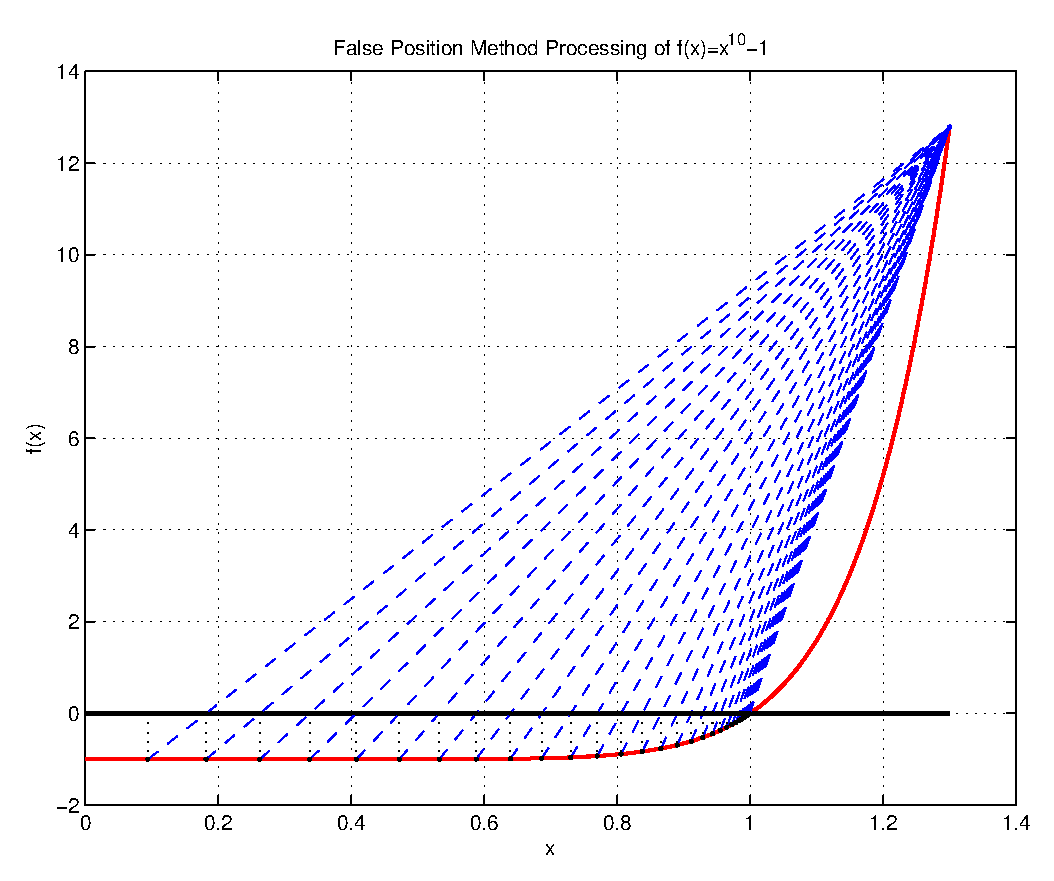
\includegraphics[keepaspectratio=true,width=0.3\linewidth]{figs/fpmprocplot.eps}}
\subfigure[Modified false position method]{
\includegraphics[keepaspectratio=true,width=0.3\linewidth]{figs/mfpmprocplot.eps}}
\caption{이분법과 가위치법 및 수정된 가위치법의 계산과정}
\label{fig:5-13-1}
\end{figure}


%
%\clearpage
%\section{개구간법\\(Open Method)}\label{sec:open}
%구간법은 미리 정의된 하한치(lower bound)와 상한치(upper bound)의 경계값으로 이루어지는 구간 내에서 근을 찾았다. 반면에 이장에서 다룰 개구간법(open methods)은 한 개의 초기값에서 시작하거나 구간 내에 근을 포함하지 않을 수도 있는 두 개의 초기값들로부터 시작하는 방법들이다. 이러한 개구간법은 종종 발산(diverge)하거나 근에서 멀어지기도 한다. 그러나 수렴(convergent)할 경우 빠르게 수렴한다.

\subsection{고정점 반복법(fixed point iteration)}
함수 $f(x)=0$의 형태를 다음 식과 같이 변형할 수 있다.
\begin{equation}\label{eq:6-1}
g(x)=x
\end{equation}
이 변형된 함수는 함수 $g$에 대한 \textsl{fixed point}의 해가 된다. 이러한 함수 $f(x)=0$에서 단순한 해법으로 재구성하는 방법은 고정점 반복(fixed point iteration)으로 이루어진다. 그러나 이러한 방법을 수행하기 이전에 우리는 변형된 함수 $g(x)=x$의 해의 존재와 유일성을 검토해야한다. 다음 정리가 이러한 질문에 대한 해를 제시한다.
\begin{theorem}[Fixed-Point Iteration]\label{theo:6-1}
함수 $g(x)$가 구간 $[a,b]$에서 연속의 함수일 때, $\forall x \in [a,b]$에 대해 $g(x)\in [a,b]$ 이면, $g$는 $[a,b]$에서 고정점(fixed point)를 갖는다. 또한, 함수 $g(x)$가 미분가능한 함수이고 아래의 식(\ref{eq:theo-1})과 같은 상수 $k<1$가 존재한다면,
\begin{equation}\label{eq:theo-1}
\left|g'(x)\right|\leq k, x \in (a,b)
\end{equation}
$g$는 정확하게 $[a,b]$에서 하나의 고정점(fixed point)를 갖는다.
\end{theorem}
구간 $[a,b]$에서 고정점을 갖는 연속함수 $g$가 주어진다면, 그 고정점(fixed point)은 구간 $[a,b]$에서 $g(x)=x$를 만족하는 $x$를 무수히 반복하여 찾을 수 있다.

\begin{algorithm}
Let $g$ be a continuous function defined on the interval $[a,b]$. The following algorithm computes a number $x_{r} \in (a,b)$ that is a solution to the equation $g(x)=x$.\\
Choose an initial guess $x_{0}$ in $[a,b]$.

\begin{algorithmic}
\For{$i=0,1,2,\cdots$}
\State $x_{i+1}=g(x_{i})$
\If{$\left|x_{i+1}-x_{i}\right|$ is sufficiently small}
\State $x_{r}=x_{i+1}$
\State \Return $x_{r}$
\EndIf
\EndFor
\end{algorithmic}
\caption{Fixed-Point Iteration}
\end{algorithm}
어떠한 환경에서 고정점 반복이 수렴해서 $x_{r}$을 찾을 수 있을까? 단순히 오차를 $e_{i}=x_{i}-x_{r}$로 가정한다면, Taylor 급수에서 $e_{i+1}\approx g'(x_{r})e_{i}$일 때, $g(x_{r})=x_{r}$임을 찾을 수 있다. 즉, $k<1$일 때, $\left|g'(x_{r})\right| \leq k$ 라면, 고정점 반복(fixed-point iteration)은 부분수렴(locally convergent)한다고 한다. 즉, 초기설정값 $x_{0}$가  $x_{r}$에 충분히 근접한 값을 선택했을 때 수렴한다는 말이다. 이러한 결과는 다음 정리를 통해 알 수 있다.

\begin{theorem}[Fixed-Point Theorem]\label{theo:6-2}
함수 $g(x)$가 구간 $[a,b]$에서 연속의 함수일 때, $\forall x \in [a,b]$에 대해 $g(x)\in [a,b]$ 이고, 다음 식과 같이 상수 $k<1$인 점이 존재한다면,
\begin{equation}\label{eq:theo-2}
\left|g'(x)\right|\leq k, x \in (a,b),
\end{equation}
반복문(the sequence of iterates) $\{x_{i}\}_{i=0}^{\infty}$는 어떤 초기가정 $x_{0} \in [a,b]$에도, 특정 고정값 $x_{r}$으로 수렴하게 된다.
\end{theorem}
함수 $g'(x)$가 수렴의 약조건 $\left|g'(x)\right|<1$에 비하여 $(a,b)$에서 $1$과 떨어지도록 경계지어야하는지에 대하여, 만약 $g'(x)$가 $x$가 어느 한점 $c \in (a,b)$로 접근할 때 $1$로의 접근을 허용한다면, 오차 $e_{i}$가 $i$가 증가할 수록 $0$으로 수렴하지 않을 수가 있다. 이러한 경우 고정점 반복법(fixed-point iteration)은 수렴하지 않는다.

일반적으로 고정점 반복(fixed-point iteration)이 수렴할 때, $\left|g'(x)\right|$의 경계치는 상수 $k$의 역으로 변화하면서 수렴한다.

한편, $f(x)=0$를 $g(x)=x$로 변환하는 식은 많은 방법이 존재하지만, 단순화된 방법으로 특정함수 $\phi(x)$를 추가한 $g(x)=x-\phi(x)f(x)$방법을 사용한다. 그러나 이러한 함수변형에 있어 가장 중요한 요소는 함수 $g(x)$의 수렴성이다.
\begin{figure}[!hbpt]
\centering
\subfigure[$g(x)=\cos(x)$]{
\includegraphics[keepaspectratio=true,width=0.4\linewidth]{figs/fpi-cos.eps}}
\subfigure[$g(x)=\exp(-x)$]{
\includegraphics[keepaspectratio=true,width=0.4\linewidth]{figs/fpi-exp.eps}}
\caption{고정점 반복법의 수렴과정}
\label{fig:6-1}
\end{figure}
\clearpage
\subsection{Newton-Raphson법 (Newton-Raphson method)}
구간법의 문제점은 적어도 한 근을 포함하는 구간을 알고있어야 한다는 점이다. 즉, 이러한 방법은 필요한 구간을 상정하기 위해서 무수히 많이 반복을 수행해야하기 때문에 실용적이지 못하다. 좀더 효과적으로 근을 구하는 방법을 찾기 위해서는 다음과 같은 질문을 해결해야 한다.
\begin{itemize}
\item Are there cases in which the problem easy to solve, and if so, how do we solve it in such cases?
\item Is it possible to apply our method of solving the problem in these "easy" cases to more general cases?
\end{itemize}
근을 구하는 공식들 중에서 가장 일반적으로 사용하는 것이 Newton-Raphson 법이다. 근에 대한 초기가정값이 $x_{i}$라면, 점 $[x_{i},f(x_{i})]$에 접하는 접선을 구할 수 있고, 이 접선이 $x$축과 교차하는 점이 개선된 근이 된다.
\ref{ch:4-1}장 \pageref{eq:4-7}페이지 식(\ref{eq:4-7})의 Taylor 급수를 통해 1차항으로 구성된 다음 식으로 근사화 시킬 수 있다.
\begin{equation}
f(x_{i+1})\cong f(x_{i})+f'(x_{i})(x_{i+1}-x_{i})
\end{equation}
즉, $x$축과의 교점에서 $f(x_{i+1})=0$이 되므로 다음과 같이 근사할 수 있다.
\begin{equation}
0=f(x_{i})+f'(x_{i})(x_{i+1}-x_{i})
\end{equation}
$x_{i+1}$에 대하여 정리하면 다음식(\ref{eq:6-6})과 같다.
\begin{equation}\label{eq:6-6}
x_{i+1}=x_{i}-\frac{f(x_{i})}{f'(x_{i})}
\end{equation}

\begin{algorithm}
Let $f:\mathbb{R}\rightarrow\mathbb{R}$ be a differentiable function. The following algorithm computes an approximate solution $x_{r}$ to the equation $f(x)=0$.\\
Choose an initial guess $x_{0}$.
\begin{algorithmic}
\For{$i=0,1,2,\cdots$}
  \If{$f(x_{i})$ is sufficiently small}
    \State $x_{r}=x_{i}$
    \State \Return $x_{r}$
  \EndIf
  \State $x_{i+1}=x_{i}-\frac{f(x_{i})}{f'(x_{i})}$
  \If{$\left|x_{i+1}-x_{i}\right|$ is sufficiently small}
    \State $x_{r}=x_{i+1}$
    \State \Return $x_{r}$
  \EndIf
\EndFor
\end{algorithmic}
\caption{Newton-Raphson Method}
\end{algorithm}
Newton-Raphson법이 수렴할때, 상당히 빨리 수렴한다. 그러나, 수렴 여부에 대해 찾기가 쉽지 않을 수 있다. 특히, 함수 $f(x)$가 근의 부근 $x_{r}$에서 수평기울기(horizontal tangent)을 가지게 될 때 반복구간에서 값이 커질 수가 있다. 이러한 경우 일반적으로 시작지점 $x_{0}$을 $x_{r}$에 가장 가까운 곳에서 선택할 필요가 있다.
\begin{theorem}[Convergence of Newton-Raphson's Method]
함수 $f(x)$를 구간 $[a,b]$에서 연속이며 미분가능하다고 가정하고, 특정한 값 $c \in [a,b]$에서 $f(c)=0$와 $f'(c)=0$을 만족한다고 가정하면, 함수 $f(x)$에 Newton-Raphson법을 적용했을때 $[c-\delta,c+\delta]$구간에서 수렴하는 어떤 초기값 $x_{0}$을 갖는 $\delta >0$인 $\delta$가 존재한다.
\end{theorem}

\framebox{예제} \textbf{Newton-Raphson법 예제 ($\sqrt{2}$ 찾기)}\\
\rule{\textwidth}{0.1pt}
다음 함수 $f(x)$를 통해 $\sqrt{2}$의 값을 Newton-Raphson법을 이용하여 예측하라.
\begin{equation}
f(x)=x^2 -2
\end{equation}
\framebox{해}
$f'(x)=2x$이기 때문에, Newton-Raphson법에서 $x_{i}$에 대한 $x_{i+1}$은 다음식과 같다.
\begin{equation}
x_{i+1}=x_{i}-\frac{f(x_{i})}{f'(x_{i})}
=x_{i}-\frac{x_{i}^2-2}{2x_{i}}
=\frac{x_{i}}{2}+\frac{1}{x_{i}}
\end{equation}

\begin{table}[!hbpt]
\centering
\begin{tabular}{l|l|l|c}
\hline
\hline
\boldmath $x_{i}$ & \boldmath $f(x_{i})$ &\boldmath $f'(x_{i})$ & \textbf{Tangent line}\\
\hline
$x_{0}=0.5 $ & $f(x_{0})=-1.75$ & $f'(x_{0})=1$ & $y=f'(x_{0})(x-x_{0})+f(x_{0})$\\
$x_{1}=2.25 $ & $f(x_{1})=3.0625$ & $f'(x_{1})=4.5$ & $y=f'(x_{1})(x-x_{1})+f(x_{1})$\\
$x_{2}=1.5694 $ &  $f(x_{2})=0.463155$ & $f'(x_{2})=3.13889$ & $y=f'(x_{2})(x-x_{2})+f(x_{2})$\\
$x_{3}=1.42189 $ & $f(x_{3})=2.177221\times10^{-2}$ & $f'(x_{3})=2.84378$ & $y=f'(x_{3})(x-x_{3})+f(x_{3})$\\
$x_{4}=1.414234 $ & $f(x_{4})=5.861552\times10^{-5}$ & $f'(x_{4})=2.82847$ & $y=f'(x_{4})(x-x_{4})+f(x_{4})$\\
\hline
\end{tabular}
\end{table}

\begin{figure}[!hbpt]
\centering
\includegraphics[keepaspectratio=true,width=0.7\textwidth]{figs/newton1.eps}
\caption{Newton-Raphson Method}
\label{fig:6-2}
\end{figure}
\clearpage
\subsection{할선법 (secant method)}
Newton-Raphson법을 수행하는데 어려운점은 바로 도함수의 계산이다. 어떤 함수에서는 도함수를 계산하는 것이 매우 어려울 수 있다. 그러한 경우 도함수는 \ref{sec:4-diff}장에서 학습한 수치미분중 후진유한제차분으로 근사시킬 수 있다. 후진차분근사법은 식(\ref{eq:4-backward})에서 도함수를 가져오기로 하자.
\begin{equation}\label{eq:6-backward}
f'(x_{i})\cong\frac{f(x_{i-1})-f(x_{i})}{x_{i-1}-x_{i}}
\end{equation}
도함수의 후진차분근사 식(\ref{eq:6-backward})을 Newton-Raphson법 식(\ref{eq:6-6})에 대입시킨다.
\begin{equation}\label{eq:6-7}
x_{i+1}=x_{i}-\frac{f(x_{i})(x_{i-1}-x_{i})}{f(x_{i-1})-f(x_{i})}
\end{equation}
식(\ref{eq:6-7})과 같이 할선법(secant method)는 두개의 초기값 $x_{i-1}$, $x_{i}$이 필요하다. 즉, $x_{2}$부터 추적해나가기 때문에 $x_{0}$과 $x_{1}$의 초기값이 필요하다.

\begin{algorithm}
Let $f:\mathbb{R}\rightarrow\mathbb{R}$ be a differentiable function. The following algorithm computes an approximate solution $x_{r}$ to the equation $f(x)=0$.\\
Choose an initial guess $x_{0}$ and $x_{1}$.
\begin{algorithmic}
\For{$i=0,1,2,\cdots$}
  \If{$f(x_{i})$ is sufficiently small}
    \State $x_{r}=x_{i}$
    \State \Return $x_{r}$
  \EndIf
  \State $x_{i+2}=x_{i+1}-\frac{f(x_{i+1})(x_{i}-x_{i+1})}{f(x_{i})-f(x_{i+1})}$
  \If{$\left|x_{i+2}-x_{i+1}\right|$ is sufficiently small}
    \State $x_{r}=x_{i+2}$
    \State \Return $x_{r}$
  \EndIf
\EndFor
\end{algorithmic}
\caption{Secant Method}
\end{algorithm}

\clearpage
\subsection{수정된 할선법 (modified secant method)}
도함수를 계산하기 위하여 임의의 두 값을 사용하기보다 $f'(x)$를 추정하기 위하여 독립변수에 약간의 변동을 주는 방법을 고려할 수 있다.
\begin{equation}
f'(x_{i})\cong \frac{f(x_{i}+\delta x_{i})-f(x_{i})}{\delta x_{i}}
\end{equation}
여기서 $\delta$는 약간의 변동량이다.식(\ref{eq:6-6})에 위의 식을 대입하면 다음과 같은 반복계산식을 얻을 수 있다.
\begin{equation}\label{eq:6-8}
x_{i+1}=x_{i}-\frac{\delta x_{i}f(x_{i})}{f(x_{i}+\delta x_{i})-f(x_{i})}
\end{equation}

\begin{algorithm}
Let $f:\mathbb{R}\rightarrow\mathbb{R}$ be a differentiable function. The following algorithm computes an approximate solution $x_{r}$ to the equation $f(x)=0$.\\
Choose an initial guess $x_{0}$ and $\delta$.
\begin{algorithmic}
\For{$i=0,1,2,\cdots$}
  \If{$f(x_{i})$ is sufficiently small}
    \State $x_{r}=x_{i}$
    \State \Return $x_{r}$
  \EndIf
  \State $x_{i+1}=x_{i}-\frac{\delta x_{i}f(x_{i})}{f(x_{i}+\delta x_{i})-f(x_{i})}$
  \If{$\left|x_{i+1}-x_{i}\right|$ is sufficiently small}
    \State $x_{r}=x_{i+1}$
    \State \Return $x_{r}$
  \EndIf
\EndFor
\end{algorithmic}
\caption{Modified Secant Method}
\end{algorithm}
이 수정된 할선법 알고리즘에서 $\delta$의 선택이 이슈가 되는데 적절하게 $\delta$를 선택하는 방법밖에는 없다. $\delta$가 작으면 식(\ref{eq:6-8})의 분모에서 발생하는 반올림 오차가 커지게되고, 또한 $\delta$가 커지게 되면 발산할 수도 있다. 그러나 적절한 $\delta$가 선택되면 도함수를 계산하기 어려운 함수의 근이나 두개의 초기가정을 결정하는 것이 어려운 경우 근을 찾는 좋은 방법이 될 수 있다.
%
%\clearpage
%\part{선형대수 방정식\\(Linear Algebraic Equations)}
%공학적 문제에서 만나는 많은 함수혹은 방정식들은 보존 법칙(conservation law)에 기초를 두고 있다. 이와 같은 법칙이 적용되는 양으로는 질량, 에너지 그리고 운동량 등이 있다. 이들 원리들은 수학적 용어를 사용하여 모델링되어지는 양(quantity)의 수준(level) 또는 응답(response)으로 표현되는 시스템의 거동(behavior)을, 시스템의 성질(property) 또는 특성(characteristic)과 외부 자극(stimuli) 또는 시스템에 작용하는 강제함수(forcing function)등에 관련시키는 평형(balance) 또는 연속방정식(continuity equation)을 이끌어내게 된다.
\ref{part1}부에서, 단일요소 시스템은 근-위치 방법들을 사용하여 풀 수 있는 단일 방정식이었다면, 다중요소 시스템은 동시에 연립하여 풀어야 할 상호 연관된 방정식으로 표현된다. 이들 방정식들은 서로 연관되어 상호 작용을 하는데 그 이유는 시스템의 한 부분이 다른 부분에 의하여 영향을 받기 때문이다. 이러한 다중요소 문제들은 집중(lumped) 또는 분산(distributed) 변수의 수학적 모델 모두에서 발생하게 된다.
\begin{figure}[!hbpt]
\centering
\subfigure[구성 요소들이 상호 연관되어 있는 집중 변수시스템(lumped variable system)]{
\includegraphics[keepaspectratio=true,width=0.8\linewidth]{figs2/pt3-1a.eps}}
\subfigure[연속체로 이루어진 분산 변수 시스템(distributed variable system]{
\includegraphics[keepaspectratio=true,width=0.8\linewidth]{figs2/pt3-1b.eps}}
\caption{선형대수 방정식을 사용하여 모델링할 수 있는 두가지 시스템}
\label{fig:pt3-1}
\end{figure}

\section{Gauss 소거법\\(Gauss elimination)}
Gauss 소거법은 연립 방정식의 해를 구하는 최초의 방법 중의 하나이지만, 현재에도 매우 중요한 알고리즘의 하나로 남아 있으며, 널리 알려져 있는 상용소프트웨어 패키지상에서 선형 방정식의 해를 구하는데 기초가 되고 있다.
\subsection{도식적 방법}
좌표의 한 축이 $x_{1}$이고, 다른 축이 $x_{2}$인 직교좌표계상에서 두 방정식을 그래프로 그린 후 그 교점으로부터 해를 얻는다.
\begin{align*}
a_{11}x_{1}+a_{12}x_{2}&=b_{1}\\
a_{21}x_{1}+a_{22}x_{2}&=b_{2}
\end{align*}
두 식을 $x_{2}$항으로 표현하여 기울기와 $x_{2}$ 절편을 얻는다.
\begin{align*}
x_{2}&=-\left(\frac{a_{11}}{a_{12}}\right)x_{1}+\frac{b_{1}}{a_{12}}\\
x_{2}&=-\left(\frac{a_{21}}{a_{22}}\right)x_{1}+\frac{b_{2}}{a_{22}}
\end{align*}
이 직선들을 직교좌표계상에서 $x_{2}$를 세로축, $x_{1}$을 가로축으로 하여 그리면, 두 선들이 만나는 점의 좌표값 $x_{1}$과 $x_{2}$가 해가 된다.
도식적 방법을 사용하여 다음 방정식을 풀면,
\begin{align*}
3x_{1}+2x_{2}&=18\\
-x_{1}+2x_{2}&=2
\end{align*}

\begin{figure}[!hbpt]
\centering
\includegraphics[keepaspectratio=true,width=0.7\linewidth]{figs2/p8_1.eps}
\caption{2개의 연립 선형대수 방정식의 도식적 방법}
\label{fig:8-1}
\end{figure}
Figure~\ref{fig:8-2}는 연립 선형 방정식을 풀 때 발생할 수 있는 세가지 경우를 보여주고 있다. Figure~\ref{fig:8-2a}는 두 개의 직선이 평행한 경우로, 두 직선이 서로 교차하지 않아 해가 존재하지 않는다. Figure~\ref{fig:8-2b}는 두 개의 직선이 일치하는 경우. 이 두 경우의 시스템을 특이(singular)하다고 한다. 특이한 경우에 매우 가까운 시스템인 Figure~\ref{fig:8-2c}의 경우는 시스템에 문제를 발생시킬 수 있는 시스템으로 불량조건(ill-conditioned)을 갖는다고 말한다.
\begin{figure}[!hbpt]
\centering
\subfigure[해가 존재하지 않는 경우]{\label{fig:8-2a}
\includegraphics[keepaspectratio=true,width=0.3\linewidth]{figs2/p8_2a.eps}}
\subfigure[해가 무한히 많은 경우]{\label{fig:8-2b}
\includegraphics[keepaspectratio=true,width=0.3\linewidth]{figs2/p8_2b.eps}}
\subfigure[불량조건 시스템]{\label{fig:8-2c}
\includegraphics[keepaspectratio=true,width=0.3\linewidth]{figs2/p8_2c.eps}}
\caption{특이하고 불량조건을 갖는 시스템}
\label{fig:8-2}
\end{figure}

\subsection{행렬식과 Cramer 공식}
Cramer 공식(Cramer's rule)은 방정식의 수가 적을 때 매우 적합한 또 다른 해법이다.Cramer 식을 수행하는데 사용될 행렬식(determinant)의 대하여 알아야 한다. 행렬식은 행렬이 불량조건인지의 여부를 판단하는데도 사용된다.
\subsubsection{행렬식}
행렬식을 다음과 같은 세 개의 연립방정식의 경우에 대하여 설명하면,
\begin{equation*}
\mathbf{AX}=\mathbf{B}
\end{equation*}
여기서 $\mathbf{A}$는 계수행렬(coefficient matrix)로써
\begin{equation*}
\mathbf{A}=\begin{bmatrix}a_{11}&a_{12}&a_{13}\\a_{21}&a_{22}&a_{23}\\a_{31}&a_{32}&a_{33}\end{bmatrix}
\end{equation*}
이 시스템의 행렬식 $D$는 다음과 같이 방정식의 계수로부터 얻어진다.
\begin{equation}\label{eq:8-2}
D=\left|\begin{array}{ccc}a_{11}&a_{12}&a_{13}\\a_{21}&a_{22}&a_{23}\\a_{31}&a_{32}&a_{33}\end{array}\right|
\end{equation}
행렬식$D$와 계수행렬$\mathbf{A}$는 같은 요소들로 구성되어 있지만, 완전히 다른 수학적 개념을 가지고 있다. 이 때문에 행렬은 bold 폰트를 사용하여 표시하고 구성요소는 대괄호를 사용하여 나타내지만 , 행렬식은 스칼라값이기 때문에 normal 폰트를 사용하고 구성요소는 절대값 괄호로 표시한다. 2차 행렬식은 다음 식(\ref{eq:8-3})과같이 표현한다.
\begin{align}
D&=\left|\begin{array}{cc}a_{11}&a_{12}\\a_{21}&a_{22}\end{array}\right|\\
&=a_{11}a_{22}-a_{12}a_{21}\label{eq:8-3}
\end{align}
3차 행렬식[식(\ref{eq:8-2})]의 경우, 행렬식의 값은 다음과 같이 계산한다.
\begin{equation}
D=a_{11}\left|\begin{array}{cc}a_{22}&a_{23}\\a_{32}&a_{33}\end{array}\right|-a_{12}\left|\begin{array}{cc}a_{21}&a_{23}\\a_{31}&a_{33}\end{array}\right|+a_{13}\left|\begin{array}{cc}a_{21}&a_{22}\\a_{31}&a_{32}\end{array}\right|
\end{equation}
여기서 $2\times2$의 행렬식을 소행렬식(minor)라고 한다.
\subsubsection{Cramer 공식}
이 공식은 연립 선형대수 방정식에서의 각각의 미지수는 두개의 행렬식의 비로 표시될 수 있다는 것을 말해준다. 다음의 $n\times n$ 연립 선형대수 방정식에서,
\begin{equation*}
\mathbf{AX}=\mathbf{B}
\end{equation*}
$n\times n$크기의 행렬 $\mathbf{A}$의 행렬식이 $0$을 가지지 않는다면, 벡터 $\mathbf{X}=(x_{1},\cdots,x_{n})^T$의 $x_{i}$는 다음 식을 통해 구할 수 있다.
\begin{equation}
x_{i}=\frac{\left|\mathbf{A}_{i}\right|}{\left|\mathbf{A}\right|}
\end{equation}
여기서, $\mathbf{A}_{i}$는 행렬 $A$의 $i$번째 열을 벡터 $\mathbf{B}$로 대체한 행렬이다.
\\
\framebox{예제} \textbf{Cramer 공식}\\
\rule{\textwidth}{0.1pt}
Cramer 공식을 사용하여 다음의 방정식을 풀어라.
\begin{align*}
0.3x_{1}+0.52x_{2}+x_{3}&=-0.01\\
0.5x_{1}+x_{2}+1.9x_{3}&=0.67\\
0.1x_{1}+0.3x_{2}+0.5x_{3}&=-0.44
\end{align*}
\framebox{해} 행렬식 $D$는 다음과 같이 쓸 수 있다.
\begin{equation*}
D=D=\left|\begin{array}{ccc}0.3&0.52&1\\0.5&1&1.9\\0.1&0.3&0.5\end{array}\right|
\end{equation*}
소행렬식을 구하면,
\begin{align*}
D_{1}&=\left|\begin{array}{cc}1&1.9\\0.3&0.5\end{array}\right|=1(0.5)-1.9(0.3)=-0.07\\
D_{2}&=\left|\begin{array}{cc}0.5&1.9\\0.1&0.5\end{array}\right|=0.5(0.5)-1.9(0.1)=0.06\\
D_{3}&=\left|\begin{array}{cc}0.5&1\\0.1&0.3\end{array}\right|=0.5(0.3)-1(0.1)=0.05
\end{align*}
$\mathbf{A}$의 행렬식은
\begin{equation*}
D=0.3(-0.07)-0.52(0.06)+1(0.05)=-0.0022
\end{equation*}
Cramer 공식을 적용하면, 해는 다음과 같이 구할 수 있다.
\begin{align*}
x_{1}&=\frac{\left|\begin{array}{ccc}-0.01&0.52&1\\0.67&1&1.9\\-0.44&0.3&0.5\end{array}\right|}{-0.0022}=\frac{0.03278}{-0.0022}=14.9\\
x_{2}&=\frac{\left|\begin{array}{ccc}0.3&-0.01&1\\0.5&0.67&1.9\\0.1&-0.44&0.5\end{array}\right|}{-0.0022}=\frac{0.0649}{-0.0022}=-29.5\\
x_{3}&=\frac{\left|\begin{array}{ccc}0.3&0.52&-0.01\\0.5&1&0.67\\0.1&0.3&-0.44\end{array}\right|}{-0.0022}=\frac{-0.04356}{-0.0022}=19.8
\end{align*}
\rule{\textwidth}{0.1pt}\\
방정식의 개수가 세 개 이상이 되면, 방정식의 개수가 증가함에 따라 행렬식을 수작업(또는 컴퓨터에 의하여)에 의하여 구하는 데에 매우 많은 시간이 소비되므로, Cramer 공식은 비현실적이라고 할 수 있다.
\subsection{Gauss 소거법}
\begin{wrapfigure}{r}{0.5\textwidth}
\centering
\includegraphics[keepaspectratio=true,width=0.48\textwidth]{figs2/p8-3.eps}
\caption{Gauss 소거법의 두단계}
\label{fig:8-3}
\end{wrapfigure}
Gauss 소거법은 전진소거(forward elimination)와 후진대입(back substitution)의 방법으로 나뉜다. 이 방법은 컴퓨터상에서 구현하기에 이상적이지만, 신뢰성 있는 알고리즘을 위하여 약간의 수정이 필요하다. 특히, 컴퓨터 프로그램에서는 0으로 나누는 경우를 피해야한다. 
다음과 같이 일반적인 $n$개의 방정식을 풀고자 한다.
\begin{align}
a_{11}x_{1}+a_{12}x_{2}+a_{13}x_{3}+\cdots+a_{1n}x_{n}&=b_{1}\label{eq:8-12a}\\
a_{21}x_{1}+a_{22}x_{2}+a_{23}x_{3}+\cdots+a_{2n}x_{n}&=b_{2}\label{eq:8-12b}\\
\vdots\qquad{}&=\vdots\nonumber\\
a_{n1}x_{1}+a_{n2}x_{2}+a_{n3}x_{3}+\cdots+a_{nn}x_{n}&=b_{n}\label{eq:8-12c}
\end{align}
\subsubsection{미지수의 전진소거(forward elimination)}
첫 번째 단계는 연립방정식을 상부삼각(upper triangular) 시스템으로 만드는 것이다. 2번째 $x_{1}$항을 소거하기 위하여 식(\ref{eq:8-12a})에 $a_{21}/a_{11}$을 곱하면,
\clearpage
\begin{equation}\label{eq:8-13}
a_{21}x_{1}+\frac{a_{21}}{a_{11}}a_{12}x_{2}+\frac{a_{21}}{a_{11}}a_{13}x_{3}+\cdots+\frac{a_{21}}{a_{11}}a_{1n}x_{n}=\frac{a_{21}}{a_{11}}b_{1}
\end{equation}
이 방정식을 식(\ref{eq:8-12b})에서 빼면,
\begin{align}
\left(a_{22}-\frac{a_{21}}{a_{11}}a_{12}\right)x_{2}+\cdots+\left(a_{2n}-\frac{a_{21}}{a_{11}}a_{1n}\right)x_{2}&=b_{2}-\frac{a_{21}}{a_{11}}b_{1}\\
a'_{22}x_{2}+\cdots+a'_{2n}x_{n}&=b'_{2}
\end{align}
이러한 방식으로 나머지 방정식에 대해서도 같은 절차를 반복한다. 그 절차를 $n-1$번을 반복수행하면,
\begin{align}
a_{11}x_{1}+a_{12}x_{2}+a_{13}x_{3}+\cdots+a_{1n}x_{n}&=b_{1}\label{eq:8-14a}\\
a'_{22}x_{2}+a'_{23}x_{3}+\cdots+a'_{2n}x_{n}&=b'_{2}\label{eq:8-14b}\\
a'_{32}x_{2}+a'_{33}x_{3}+\cdots+a'_{3n}x_{n}&=b'_{3}\label{eq:8-14c}\\ 
\vdots\qquad{}&=\vdots\nonumber\\
a'_{n2}x_{2}+a'_{n3}x_{3}+\cdots+a'_{nn}x_{n}&=b'_{n}\label{eq:8-14d}
\end{align}
식(\ref{8-12a})를 피벗방정식(pivot equation)이라고 하고, $a_{11}$을 피벗계수(pivot coefficient) 또는 피벗요소(pivot element)라고 한다. 계속해서 식(\ref{eq:8-14b})를 시작으로 나머지 피벗방정식을 아래로 내리면서 소거를 해나갈 수 있다. 이 과정에서 마지막 작업은 $n$번째 방정식으로부터 $x_{n-1}$을 소거하기 위하여 $(n-1)$번째 방정식을 사용하는 것이다. 이 시점에서 시스템은 상부삼각(upper triangular) 시스템으로 변환된다.
\begin{align}
a_{11}x_{1}+a_{12}x_{2}+a_{13}x_{3}+\cdots+a_{1n}x_{n}&=b_{1}\label{eq:8-15a}\\
a'_{22}x_{2}+a'_{23}x_{3}+\cdots+a'_{2n}x_{n}&=b'_{2}\label{eq:8-15b}\\
a''_{33}x_{3}+\cdots+a''_{3n}x_{n}&=b''_{3}\label{eq:8-15c}\\
\ddots\qquad{}&=\vdots\nonumber\\
a_{nn}^{(n-1)}x_{n}&=b_{n}^{(n-1)\label{eq:8-15d}}
\end{align}
\subsubsection{후진대입(back substitution)}
식(\ref{eq:8-15d})는 $x_{n}$값을 얻는데 사용할 수 있다.
\begin{equation}\label{eq:8-16}
x_{n}=\frac{b_{n}^{(n-1)}}{a_{nn}^{(n-1)}}
\end{equation}
이 결과를 $(n-1)$번째 방정식에 대입하여 $x_{n-1}$을 얻게 된다. 나머지 $x$들의 값을 얻기 위하여 반복되는 이 후진대입의 과정은 다음 식과 같다.
\begin{equation}\label{eq:8-17}
x_{i}=\frac{b_{i}^{(i-1)}-\sum\limits_{j=i+1}^{n}a_{ij}^{(i-1)}x_{j}}{a_{ii}^{(i-1)}}\quad\text{for $i=n-1$, $n-2$, $\cdots$, $1$}
\end{equation}

\begin{algorithm}
Let loop $k$ control the elimination step, loop $i$ control $i-$th row accessing and loop $j$ control $j-$th column accessing, the sequential Gaussian Elimination alogithms is decribed as follow(in numerical program, vector $\mathbf{B}$ is stored as $(n+1)-$th column of matrix $\mathbf{A}$):
\begin{algorithmic}
\For{$k=1$ to $n-1$}
  \For{$i=k+1$ to $n$}
    \State $a_{ik}=a_{ik}/a_{kk}$;
    \For{$j=k+1$ to $n+1$}
      \State $a_{ij}=a_{ij}-a_{ik}\times a_{kj}$;
    \EndFor
  \EndFor
\EndFor
\end{algorithmic}
Note that since the entries in the lower triangluar matrix vanish after elimination, their space is used to store multipliers $a_{ik}=a_{ik}/a_{kk}$
\caption{Forward Elimination}
\end{algorithm}

\begin{algorithm}
\begin{algorithmic}
\For{$i=n$ to $1$}
  \For{$j=i+1$ to $n$}
    \State $x_{i}=x_{i}-a_{ij}\times x_{j}$;
  \EndFor
  \State $x_{i}=x_{i}/a_{ii}$;
\EndFor
\end{algorithmic}
Note that $x_{i}$ is stored in the space of $a_{i,n+1}$.
\caption{Backward Substitution}
\end{algorithm}
\subsection{피벗화}
피벗요소가 0인 경우에는 정규화 과정에서 0으로 나누는 경우가 발생하고 0이 아닌경우에도 0에 가까운 피벗일 수록 반올림오차가 생겨날 수 있기 때문에 문제가 발생할 수 있다. 따라서, 각 행들이 정규화되기 전에, 피벗요소 아래에 열중에 가장 큰 계수를 찾은 후, 가장 큰 요소가 피벗요소가 되도록 행의 위치를 교환하여야 한다. 이를 부분피벗화(partial pivoting)라고 한다. 만일 행뿐만 아니라 열에서도 가장 큰 요소를 찾아 위치교환을 한다면, 완전피벗화(complete pivoting)라고 부른다.



%\subsection{Gauss-Jordan법}
%Gauss-Jordan법은 Gauss 소거법의 변형으로 차이점은 피벗요소 밑에 있는 방정식뿐만 아니라 모든 방정식으로 부터 미지수가 소거된다. 또 모든 행을 각각의 피멋요소로 나누어 정규화된다. 따라서 소거단계의 결과로 삼각행렬이 아닌 단위행렬(identity matrix)을 얻게 된다. 결과적으로 이 방법의에서는 해를 구하기 위하여 후진대입을 할 필요가 없다.
%\begin{equation}
%\begin{bmatrix}a_{11}&a_{12}&a_{13}&\vdots&b_{1}\\a_{21}&a_{22}&a_{23}&\vdots&b_{2}\\a_{31}&a_{32}&a_{33}&\vdots&b_{3}\end{bmatrix}\leftarrow
%\end{equation}


%\begin{equation*}
%\begin{bmatrix}a_{11}&a_{12}&a_{13}&b_{1}\\a_{21}&a_{22}&a_{23}&b_{2}\\a_{31}&a_{32}&a_{33}&b_{3}\end{bmatrix}
%\end{equation*}
%\begin{equation*}
%\begin{bmatrix}a_{11}&a_{12}&a_{13}&b_{1}\\&a'_{22}&a'_{23}&b'_{2}\\&&a''_{33}&b''_{3}\end{bmatrix}
%\end{equation*}
%\begin{align*}
%x_{3}&=b''_{3}/a''_{33}\\
%x_{2}&=\left(b'_{2}-a'_{23}x_{3}\right)/a'_{22}\\
%x_{1}&=\left(b_{1}-a_{12}x_{2}-a_{13}x_{3}\right)/a_{11}
%\end{align*}

%
%\clearpage
%\section{LU분해법과 역행렬\\(LU Decomposition and Matrix Inversion)}
%LU분해법의 주요 장점은, 많은 시간이 소비되는 소거 단계를 공식화함으로써 계수행렬 $\mathbf{A}$에만 연산을 수행한다는 것이다. 따라서, 이 방법은 $\mathbf{A}$가 주어지고, 여러가지 다른 값을 가지는 우변벡터 $\mathbf{B}$를 사용하여 반복적으로 해를 구하는 경우에 적합하다.
\begin{equation}\label{eq:9-1}
\mathbf{Ax}=\mathbf{B}
\end{equation}
Gauss소거법은 전진소거와 후진대입이라는 두 단계로 이루어져 있는데, 이 중에 전진소거 단계에서 많은 계산시간이 요구된다. 이는 특히 방정식의 수가 많은 경우에 더욱 그러하다. LU분해법(LU decomposition method)으로 시간이 많이 걸리는 $\mathbf{A}$의 소거 과정과 우변벡터 $\mathbf{B}$에 대한 소거 과정이 분리되게 된다. 따라서, $\mathbf{A}$가 처음에 한번만 "분해된다면(decompose)", 우변벡터가 계속 바뀌는 경우에 대해서도 효율적으로 해를 구할 수 있게 된다.
\begin{equation}\label{eq:9-2}
\mathbf{Ax}-\mathbf{B}=0
\end{equation}
식(\ref{eq:9-2})가 상부삼각 시스템으로 표시될 수 있다고 가정하면,
\begin{equation}\label{eq:9-3}
\begin{bmatrix}u_{11}&u_{12}&u_{13}\\0&u_{22}&u_{23}\\0&0&u_{33}\end{bmatrix}\begin{Bmatrix}x_{1}\\x_{2}\\x_{3}\end{Bmatrix}=\begin{Bmatrix}d_{1}\\d_{2}\\d_{3}\end{Bmatrix}
\end{equation}
이는 Gauss 소거법의 첫 번째 단계에서 수행되는 과정과 유사하다. 즉, 소거 과정을 통해 주어진 시스템이 상부삼각 형태로 변환된다. 식(\ref{eq:9-3})은 다음과 같이 표시될 수 있다.
\begin{equation}\label{eq:9-4}
\mathbf{Ux}-\mathbf{D}=0
\end{equation}
여기서 다음과 같이 대각선에 1의 값을 가지는 하부삼각행렬이 있다고 가정하고
\begin{equation}\label{eq:9-5}
\mathbf{L}=\begin{bmatrix}1&0&0\\l_{21}&1&0\\l_{31}&l_{32}&1\end{bmatrix}
\end{equation}
이를 식(\ref{eq:9-4})에 곱하면 식(\ref{eq:9-2})의 결과가 얻어진다고 가정하자. 즉,
\begin{equation}\label{eq:9-6}
\mathbf{L}\left(\mathbf{Ux}-\mathbf{D}\right)=\mathbf{Ax}-\mathbf{B}
\end{equation}
만일 위 방정식이 성립한다면, 행렬의 곱셈 법칙으로부터 다음과 같은 결과를 얻는다.
\begin{align}
\mathbf{LU}&=\mathbf{A}\label{eq:9-7}\\
\mathbf{LD}&=\mathbf{B}\label{eq:9-8}
\end{align}
식(\ref{eq:9-4}),(\ref{eq:9-7}),(\ref{eq:9-8})을 기초로 하여, 해를 구하기 위한 두 단계 전략을 구성한다.
\begin{itemize}
\item[1] \textbf{LU분해단계 : } $\mathbf{A}$를 하부삼각행렬 $\mathbf{L}$와 상부삼각행렬 $\mathbf{U}$로 분해한다.
\item[2] \textbf{대입단계 : } $\mathbf{L}$과 $\mathbf{U}$를 사용하여 주어진 우변벡터 $\mathbf{B}$에 대한 해 $\mathbf{x}$를 구한다. 이 과정은 다시 두 단계로 구성된다. 먼저, 식(\ref{eq:9-8})을 이용하여 벡터 $\mathbf{D}$를 전진대입하여 구한다. 그리고, 그 결과를 식(\ref{eq:9-4})에 대입한 후 후진대입으로 $\mathbf{x}$를 구한다.
\end{itemize}

\begin{algorithm}
\begin{algorithmic}
\Function{Decompose}{$a\in\mathbf{A}$,$n$}
\For{$k=1$ to $n-1$}
  \For{$i=k+1$ to $n$}
    \State $a_{ik}=a_{ik}/a_{kk}$;
    \For{$j=k+1$ to $n+1$}
      \State $a_{ij}=a_{ij}-a_{ik}\times a_{kj}$;
    \EndFor
  \EndFor
\EndFor
\EndFunction
\end{algorithmic}
\caption{LU Decompose}
\end{algorithm}

\begin{algorithm}
\begin{algorithmic}
\Function{Substitute}{$a\in\mathbf{A}$,$n$,$b\in\mathbf{B}$,$x\in\mathbf{x}$}
\Comment{Forward substitution}
\For{$i=2$ to $n$}
  \State $sum=b_{i}$
  \For{$j=1$ to $i-1$}
    \State $sum=sum-a_{ij}\times b_{i}$
  \EndFor
  \State $b_{i}=sum$
\EndFor
\Comment{Back substitution}
\State $x_{n}=b_{n}/a_{nn}$
\For{$i=n-1:-1:1$}
  \State $sum=0$
  \For{$j=i+1$ to $n$}
    \State $sum=sum+a_{ij}\times x_{j}$
  \EndFor
  \State $x_{i}=(b_{i}-sum)/a_{ij}$
\EndFor
\EndFunction
\end{algorithmic}
\caption{Substitution}
\end{algorithm}
\subsection{역행렬}
LU분해의 가장 큰 강점은 여러개의 우변벡터에 대하여 효율적으로 해를 구할 수 있다는 것이다. 즉, 이방법은 역행렬을 구하기 위하여 여러개의 단위벡터를 가지고 계산하는 경우에 이상적이라고 할 수 있다.
\\
\framebox{예제} \textbf{역행렬}\\
\rule{\textwidth}{0.1pt}
LU분해를 사용하여 다음 $\mathbf{A}$행렬의 역행렬을 구하라.
\begin{equation*}
\mathbf{A}=\begin{bmatrix}3&-0.2&-0.2\\0.1&7&-0.3\\0.3&-0.2&10\end{bmatrix}
\end{equation*}
LU분해를 하여 다음과 같은 상부, 하부삼각행렬을 얻을 수 있다.
\begin{align*}
\mathbf{U}&=\begin{bmatrix}3&-0.1&-0.2\\0&7.00333&-0.293333\\0&0&10.0120\end{bmatrix}\\
\mathbf{L}&=\begin{bmatrix}1&0&0\\0.0333333&1&0\\0.100000&-0.0271300&1\end{bmatrix}\\
\end{align*}
\framebox{해} 단위벡터(첫 번째 행에 1이 있음)를 우변벡터로 놓고, 전진대입하여 해를 구함으로써 역행렬의 첫 번째 열이 계산된다. 즉, 하부삼각행렬인 식(\ref{eq:9-8})을 다음과 같이 놓을 수 있다.
\begin{equation*}
\begin{bmatrix}1&0&0\\0.0333333&1&0\\0.100000&-0.0271300&1\end{bmatrix}\begin{Bmatrix}d_{1}\\d_{2}\\d_{3}\end{Bmatrix}=\begin{Bmatrix}1\\0\\0\end{Bmatrix}
\end{equation*}
전진대입으로 해를 구하면 $\mathbf{D}^{T}=[1,-0.03333,-0.1009]$가 된다. 이 벡터를 식(\ref{eq:9-3})의 우변으로 사용하면,
\begin{equation*}
\begin{bmatrix}3&-0.1&-0.2\\0&7.00333&-0.293333\\0&0&10.0120\end{bmatrix}\begin{Bmatrix}x_{1}\\x_{2}\\x_{3}\end{Bmatrix}=\begin{Bmatrix}1\\-0.03333\\0.1009\end{Bmatrix}
\end{equation*}
위 식을 후진대입으로 풀면, $\mathbf{x}^{T}=[0.33249,-0.00518,-0.01008]$을 얻게 되어 역행렬의 첫 번째 열은,
\begin{equation*}
\mathbf{A}^{-1}=\begin{bmatrix}0.33249&0&0\\-0.00518&0&0\\-0.01008&0&0\end{bmatrix}
\end{equation*}
역행렬의 두 번째 열을 결정하기 위하여, 식(\ref{eq:9-8})을 다음과 같이 공식화한다.
\begin{equation*}
\begin{bmatrix}1&0&0\\0.0333333&1&0\\0.100000&-0.0271300&1\end{bmatrix}\begin{Bmatrix}d_{1}\\d_{2}\\d_{3}\end{Bmatrix}=\begin{Bmatrix}0\\1\\0\end{Bmatrix}
\end{equation*}
위 식을 $\mathbf{D}$에 대하여 풀고, 식(\ref{eq:9-3})을 사용하여 $\mathbf{x}^{T}=[0.3004944,0.142903,0.00271]$을 구해, 역행렬의 두 번째 열은 다음과 같이 된다.
\begin{equation*}
\mathbf{A}^{-1}=\begin{bmatrix}0.33249&0.004944&0\\-0.00518&0.142903&0\\-0.01008&0.00271&0\end{bmatrix}
\end{equation*}
마지막으로 $\mathbf{B}=[0,0,1]$을 사용하여 전진, 후진대입으로 해를 구하면, $\mathbf{x}^{T}=[0.006798,0.004183,0.09988]$을 얻게 되므로, 역행렬의 마지막 열은 다음과 같이 된다.
\begin{equation*}
\mathbf{A}^{-1}=\begin{bmatrix}0.33249&0.004944&0.006798\\-0.00518&0.142903&0.004183\\-0.01008&0.00271&0.09988\end{bmatrix}
\end{equation*}
이 결과에 대한 검증은 $\mathbf{AA}^{-1}=\mathbf{I}$가 되는 것을 보임으로써 증명할 수 있다.\\
\rule{\textwidth}{0.1pt}
%Gauss 소거법에서와 같이 LU분해에서도 0으로 나누는 경우를 피하기 위한 피벗화를 수행하여야 한다. 
%공학적 문제에서 만나는 많은 함수혹은 방정식들은 보존 법칙(conservation law)에 기초를 두고 있다. 이와 같은 법칙이 적용되는 양으로는 질량, 에너지 그리고 운동량 등이 있다. 이들 원리들은 수학적 용어를 사용하여 모델링되어지는 양(quantity)의 수준(level) 또는 응답(response)으로 표현되는 시스템의 거동(behavior)을, 시스템의 성질(property) 또는 특성(characteristic)과 외부 자극(stimuli) 또는 시스템에 작용하는 강제함수(forcing function)등에 관련시키는 평형(balance) 또는 연속방정식(continuity equation)을 이끌어내게 된다.
%\ref{part1}부에서, 단일요소 시스템은 근-위치 방법들을 사용하여 풀 수 있는 단일 방정식이었다면, 다중요소 시스템은 동시에 연립하여 풀어야 할 상호 연관된 방정식으로 표현된다. 이들 방정식들은 서로 연관되어 상호 작용을 하는데 그 이유는 시스템의 한 부분이 다른 부분에 의하여 영향을 받기 때문이다. 이러한 다중요소 문제들은 집중(lumped) 또는 분산(distributed) 변수의 수학적 모델 모두에서 발생하게 된다.
%\begin{figure}[!hbpt]
%\centering
%\subfigure[구성 요소들이 상호 연관되어 있는 집중 변수시스템(lumped variable system)]{
%\includegraphics[keepaspectratio=true,width=0.8\linewidth]{figs2/pt3-1a.eps}}
%\subfigure[연속체로 이루어진 분산 변수 시스템(distributed variable system]{
%\includegraphics[keepaspectratio=true,width=0.8\linewidth]{figs2/pt3-1b.eps}}
%\caption{선형대수 방정식을 사용하여 모델링할 수 있는 두가지 시스템}
%\label{fig:pt3-1}
%\end{figure}
%
%\section{Gauss 소거법(Gauss elimination)}
%Gauss 소거법은 연립 방정식의 해를 구하는 최초의 방법 중의 하나이지만, 현재에도 매우 중요한 알고리즘의 하나로 남아 있으며, 널리 알려져 있는 상용소프트웨어 패키지상에서 선형 방정식의 해를 구하는데 기초가 되고 있다.
%\subsection{도식적 방법}
%좌표의 한 축이 $x_{1}$이고, 다른 축이 $x_{2}$인 직교좌표계상에서 두 방정식을 그래프로 그린 후 그 교점으로부터 해를 얻는다.
%\begin{align*}
%a_{11}x_{1}+a_{12}x_{2}&=b_{1}\\
%a_{21}x_{1}+a_{22}x_{2}&=b_{2}
%\end{align*}
%두 식을 $x_{2}$항으로 표현하여 기울기와 $x_{2}$ 절편을 얻는다.
%\begin{align*}
%x_{2}&=-\left(\frac{a_{11}}{a_{12}}\right)x_{1}+\frac{b_{1}}{a_{12}}\\
%x_{2}&=-\left(\frac{a_{21}}{a_{22}}\right)x_{1}+\frac{b_{2}}{a_{22}}
%\end{align*}
%이 직선들을 직교좌표계상에서 $x_{2}$를 세로축, $x_{1}$을 가로축으로 하여 그리면, 두 선들이 만나는 점의 좌표값 $x_{1}$과 $x_{2}$가 해가 된다.
%도식적 방법을 사용하여 다음 방정식을 풀면,
%\begin{align*}
%3x_{1}+2x_{2}&=18\\
%-x_{1}+2x_{2}&=2
%\end{align*}
%
%\begin{figure}[!hbpt]
%\centering
%\includegraphics[keepaspectratio=true,width=0.7\linewidth]{figs2/p8_1.eps}
%\caption{2개의 연립 선형대수 방정식의 도식적 방법}
%\label{fig:8-1}
%\end{figure}
%Figure~\ref{fig:8-2}는 연립 선형 방정식을 풀 때 발생할 수 있는 세가지 경우를 보여주고 있다. Figure~\ref{fig:8-2a}는 두 개의 직선이 평행한 경우로, 두 직선이 서로 교차하지 않아 해가 존재하지 않는다. Figure~\ref{fig:8-2b}는 두 개의 직선이 일치하는 경우. 이 두 경우의 시스템을 특이(singular)하다고 한다. 특이한 경우에 매우 가까운 시스템인 Figure~\ref{fig:8-2c}의 경우는 시스템에 문제를 발생시킬 수 있는 시스템으로 불량조건(ill-conditioned)을 갖는다고 말한다.
%\begin{figure}[!hbpt]
%\centering
%\subfigure[해가 존재하지 않는 경우]{\label{fig:8-2a}
%\includegraphics[keepaspectratio=true,width=0.3\linewidth]{figs2/p8_2a.eps}}
%\subfigure[해가 무한히 많은 경우]{\label{fig:8-2b}
%\includegraphics[keepaspectratio=true,width=0.3\linewidth]{figs2/p8_2b.eps}}
%\subfigure[불량조건 시스템]{\label{fig:8-2c}
%\includegraphics[keepaspectratio=true,width=0.3\linewidth]{figs2/p8_2c.eps}}
%\caption{특이하고 불량조건을 갖는 시스템}
%\label{fig:8-2}
%\end{figure}
%
%\subsection{행렬식과 Cramer 공식}
%Cramer 공식(Cramer's rule)은 방정식의 수가 적을 때 매우 적합한 또 다른 해법이다.Cramer 식을 수행하는데 사용될 행렬식(determinant)의 대하여 알아야 한다. 행렬식은 행렬이 불량조건인지의 여부를 판단하는데도 사용된다.
%\subsubsection{행렬식}
%행렬식을 다음과 같은 세 개의 연립방정식의 경우에 대하여 설명하면,
%\begin{equation*}
%\mathbf{AX}=\mathbf{B}
%\end{equation*}
%여기서 $\mathbf{A}$는 계수행렬(coefficient matrix)로써
%\begin{equation*}
%\mathbf{A}=\begin{bmatrix}a_{11}&a_{12}&a_{13}\\a_{21}&a_{22}&a_{23}\\a_{31}&a_{32}&a_{33}\end{bmatrix}
%\end{equation*}
%이 시스템의 행렬식 $D$는 다음과 같이 방정식의 계수로부터 얻어진다.
%\begin{equation}\label{eq:8-2}
%D=\left|\begin{array}{ccc}a_{11}&a_{12}&a_{13}\\a_{21}&a_{22}&a_{23}\\a_{31}&a_{32}&a_{33}\end{array}\right|
%\end{equation}
%행렬식$D$와 계수행렬$\mathbf{A}$는 같은 요소들로 구성되어 있지만, 완전히 다른 수학적 개념을 가지고 있다. 이 때문에 행렬은 bold 폰트를 사용하여 표시하고 구성요소는 대괄호를 사용하여 나타내지만 , 행렬식은 스칼라값이기 때문에 normal 폰트를 사용하고 구성요소는 절대값 괄호로 표시한다. 2차 행렬식은 다음 식(\ref{eq:8-3})과같이 표현한다.
%\begin{align}
%D&=\left|\begin{array}{cc}a_{11}&a_{12}\\a_{21}&a_{22}\end{array}\right|\\
%&=a_{11}a_{22}-a_{12}a_{21}\label{eq:8-3}
%\end{align}
%3차 행렬식[식(\ref{eq:8-2})]의 경우, 행렬식의 값은 다음과 같이 계산한다.
%\begin{equation}
%D=a_{11}\left|\begin{array}{cc}a_{22}&a_{23}\\a_{32}&a_{33}\end{array}\right|-a_{12}\left|\begin{array}{cc}a_{21}&a_{23}\\a_{31}&a_{33}\end{array}\right|+a_{13}\left|\begin{array}{cc}a_{21}&a_{22}\\a_{31}&a_{32}\end{array}\right|
%\end{equation}
%여기서 $2\times2$의 행렬식을 소행렬식(minor)라고 한다.
%\subsubsection{Cramer 공식}
%이 공식은 연립 선형대수 방정식에서의 각각의 미지수는 두개의 행렬식의 비로 표시될 수 있다는 것을 말해준다. 다음의 $n\times n$ 연립 선형대수 방정식에서,
%\begin{equation*}
%\mathbf{AX}=\mathbf{B}
%\end{equation*}
%$n\times n$크기의 행렬 $\mathbf{A}$의 행렬식이 $0$을 가지지 않는다면, 벡터 $\mathbf{X}=(x_{1},\cdots,x_{n})^T$의 $x_{i}$는 다음 식을 통해 구할 수 있다.
%\begin{equation}
%x_{i}=\frac{\left|\mathbf{A}_{i}\right|}{\left|\mathbf{A}\right|}
%\end{equation}
%여기서, $\mathbf{A}_{i}$는 행렬 $A$의 $i$번째 열을 벡터 $\mathbf{B}$로 대체한 행렬이다.
%\\
%\framebox{예제} \textbf{Cramer 공식}\\
%\rule{\textwidth}{0.1pt}
%Cramer 공식을 사용하여 다음의 방정식을 풀어라.
%\begin{align*}
%0.3x_{1}+0.52x_{2}+x_{3}&=-0.01\\
%0.5x_{1}+x_{2}+1.9x_{3}&=0.67\\
%0.1x_{1}+0.3x_{2}+0.5x_{3}&=-0.44
%\end{align*}
%\framebox{해} 행렬식 $D$는 다음과 같이 쓸 수 있다.
%\begin{equation*}
%D=D=\left|\begin{array}{ccc}0.3&0.52&1\\0.5&1&1.9\\0.1&0.3&0.5\end{array}\right|
%\end{equation*}
%소행렬식을 구하면,
%\begin{align*}
%D_{1}&=\left|\begin{array}{cc}1&1.9\\0.3&0.5\end{array}\right|=1(0.5)-1.9(0.3)=-0.07\\
%D_{2}&=\left|\begin{array}{cc}0.5&1.9\\0.1&0.5\end{array}\right|=0.5(0.5)-1.9(0.1)=0.06\\
%D_{3}&=\left|\begin{array}{cc}0.5&1\\0.1&0.3\end{array}\right|=0.5(0.3)-1(0.1)=0.05
%\end{align*}
%$\mathbf{A}$의 행렬식은
%\begin{equation*}
%D=0.3(-0.07)-0.52(0.06)+1(0.05)=-0.0022
%\end{equation*}
%Cramer 공식을 적용하면, 해는 다음과 같이 구할 수 있다.
%\begin{align*}
%x_{1}&=\frac{\left|\begin{array}{ccc}-0.01&0.52&1\\0.67&1&1.9\\-0.44&0.3&0.5\end{array}\right|}{-0.0022}=\frac{0.03278}{-0.0022}=14.9\\
%x_{2}&=\frac{\left|\begin{array}{ccc}0.3&-0.01&1\\0.5&0.67&1.9\\0.1&-0.44&0.5\end{array}\right|}{-0.0022}=\frac{0.0649}{-0.0022}=-29.5\\
%x_{3}&=\frac{\left|\begin{array}{ccc}0.3&0.52&-0.01\\0.5&1&0.67\\0.1&0.3&-0.44\end{array}\right|}{-0.0022}=\frac{-0.04356}{-0.0022}=19.8
%\end{align*}
%\rule{\textwidth}{0.1pt}\\
%방정식의 개수가 세 개 이상이 되면, 방정식의 개수가 증가함에 따라 행렬식을 수작업(또는 컴퓨터에 의하여)에 의하여 구하는 데에 매우 많은 시간이 소비되므로, Cramer 공식은 비현실적이라고 할 수 있다.
%\subsection{Gauss 소거법}
%\begin{wrapfigure}{r}{0.5\textwidth}
%\centering
%\includegraphics[keepaspectratio=true,width=0.48\textwidth]{figs2/p8-3.eps}
%\caption{Gauss 소거법의 두단계}
%\label{fig:8-3}
%\end{wrapfigure}
%Gauss 소거법은 전진소거(forward elimination)와 후진대입(back substitution)의 방법으로 나뉜다. 이 방법은 컴퓨터상에서 구현하기에 이상적이지만, 신뢰성 있는 알고리즘을 위하여 약간의 수정이 필요하다. 특히, 컴퓨터 프로그램에서는 0으로 나누는 경우를 피해야한다. 
%다음과 같이 일반적인 $n$개의 방정식을 풀고자 한다.
%\begin{align}
%a_{11}x_{1}+a_{12}x_{2}+a_{13}x_{3}+\cdots+a_{1n}x_{n}&=b_{1}\label{eq:8-12a}\\
%a_{21}x_{1}+a_{22}x_{2}+a_{23}x_{3}+\cdots+a_{2n}x_{n}&=b_{2}\label{eq:8-12b}\\
%\vdots\qquad{}&=\vdots\nonumber\\
%a_{n1}x_{1}+a_{n2}x_{2}+a_{n3}x_{3}+\cdots+a_{nn}x_{n}&=b_{n}\label{eq:8-12c}
%\end{align}
%\subsubsection{미지수의 전진소거(forward elimination)}
%첫 번째 단계는 연립방정식을 상부삼각(upper triangular) 시스템으로 만드는 것이다. 2번째 $x_{1}$항을 소거하기 위하여 식(\ref{eq:8-12a})에 $a_{21}/a_{11}$을 곱하면,
%\clearpage
%\begin{equation}\label{eq:8-13}
%a_{21}x_{1}+\frac{a_{21}}{a_{11}}a_{12}x_{2}+\frac{a_{21}}{a_{11}}a_{13}x_{3}+\cdots+\frac{a_{21}}{a_{11}}a_{1n}x_{n}=\frac{a_{21}}{a_{11}}b_{1}
%\end{equation}
%이 방정식을 식(\ref{eq:8-12b})에서 빼면,
%\begin{align}
%\left(a_{22}-\frac{a_{21}}{a_{11}}a_{12}\right)x_{2}+\cdots+\left(a_{2n}-\frac{a_{21}}{a_{11}}a_{1n}\right)x_{2}&=b_{2}-\frac{a_{21}}{a_{11}}b_{1}\\
%a'_{22}x_{2}+\cdots+a'_{2n}x_{n}&=b'_{2}
%\end{align}
%이러한 방식으로 나머지 방정식에 대해서도 같은 절차를 반복한다. 그 절차를 $n-1$번을 반복수행하면,
%\begin{align}
%a_{11}x_{1}+a_{12}x_{2}+a_{13}x_{3}+\cdots+a_{1n}x_{n}&=b_{1}\label{eq:8-14a}\\
%a'_{22}x_{2}+a'_{23}x_{3}+\cdots+a'_{2n}x_{n}&=b'_{2}\label{eq:8-14b}\\
%a'_{32}x_{2}+a'_{33}x_{3}+\cdots+a'_{3n}x_{n}&=b'_{3}\label{eq:8-14c}\\ 
%\vdots\qquad{}&=\vdots\nonumber\\
%a'_{n2}x_{2}+a'_{n3}x_{3}+\cdots+a'_{nn}x_{n}&=b'_{n}\label{eq:8-14d}
%\end{align}
%식(\ref{8-12a})를 피벗방정식(pivot equation)이라고 하고, $a_{11}$을 피벗계수(pivot coefficient) 또는 피벗요소(pivot element)라고 한다. 계속해서 식(\ref{eq:8-14b})를 시작으로 나머지 피벗방정식을 아래로 내리면서 소거를 해나갈 수 있다. 이 과정에서 마지막 작업은 $n$번째 방정식으로부터 $x_{n-1}$을 소거하기 위하여 $(n-1)$번째 방정식을 사용하는 것이다. 이 시점에서 시스템은 상부삼각(upper triangular) 시스템으로 변환된다.
%\begin{align}
%a_{11}x_{1}+a_{12}x_{2}+a_{13}x_{3}+\cdots+a_{1n}x_{n}&=b_{1}\label{eq:8-15a}\\
%a'_{22}x_{2}+a'_{23}x_{3}+\cdots+a'_{2n}x_{n}&=b'_{2}\label{eq:8-15b}\\
%a''_{33}x_{3}+\cdots+a''_{3n}x_{n}&=b''_{3}\label{eq:8-15c}\\
%\ddots\qquad{}&=\vdots\nonumber\\
%a_{nn}^{(n-1)}x_{n}&=b_{n}^{(n-1)\label{eq:8-15d}}
%\end{align}
%\subsubsection{후진대입(back substitution)}
%식(\ref{eq:8-15d})는 $x_{n}$값을 얻는데 사용할 수 있다.
%\begin{equation}\label{eq:8-16}
%x_{n}=\frac{b_{n}^{(n-1)}}{a_{nn}^{(n-1)}}
%\end{equation}
%이 결과를 $(n-1)$번째 방정식에 대입하여 $x_{n-1}$을 얻게 된다. 나머지 $x$들의 값을 얻기 위하여 반복되는 이 후진대입의 과정은 다음 식과 같다.
%\begin{equation}\label{eq:8-17}
%x_{i}=\frac{b_{i}^{(i-1)}-\sum\limits_{j=i+1}^{n}a_{ij}^{(i-1)}x_{j}}{a_{ii}^{(i-1)}}\quad\text{for $i=n-1$, $n-2$, $\cdots$, $1$}
%\end{equation}
%
%\begin{algorithm}
%Let loop $k$ control the elimination step, loop $i$ control $i-$th row accessing and loop $j$ control $j-$th column accessing, the sequential Gaussian Elimination alogithms is decribed as follow(in numerical program, vector $\mathbf{B}$ is stored as $(n+1)-$th column of matrix $\mathbf{A}$):
%\begin{algorithmic}
%\For{$k=1$ to $n-1$}
%  \For{$i=k+1$ to $n$}
%    \State $a_{ik}=a_{ik}/a_{kk}$;
%    \For{$j=k+1$ to $n+1$}
%      \State $a_{ij}=a_{ij}-a_{ik}\times a_{kj}$;
%    \EndFor
%  \EndFor
%\EndFor
%\end{algorithmic}
%Note that since the entries in the lower triangluar matrix vanish after elimination, their space is used to store multipliers $a_{ik}=a_{ik}/a_{kk}$
%\caption{Forward Elimination}
%\end{algorithm}
%
%\begin{algorithm}
%\begin{algorithmic}
%\For{$i=n$ to $1$}
%  \For{$j=i+1$ to $n$}
%    \State $x_{i}=x_{i}-a_{ij}\times x_{j}$;
%  \EndFor
%  \State $x_{i}=x_{i}/a_{ii}$;
%\EndFor
%\end{algorithmic}
%Note that $x_{i}$ is stored in the space of $a_{i,n+1}$.
%\caption{Backward Substitution}
%\end{algorithm}
%\subsection{피벗화}
%피벗요소가 0인 경우에는 정규화 과정에서 0으로 나누는 경우가 발생하고 0이 아닌경우에도 0에 가까운 피벗일 수록 반올림오차가 생겨날 수 있기 때문에 문제가 발생할 수 있다. 따라서, 각 행들이 정규화되기 전에, 피벗요소 아래에 열중에 가장 큰 계수를 찾은 후, 가장 큰 요소가 피벗요소가 되도록 행의 위치를 교환하여야 한다. 이를 부분피벗화(partial pivoting)라고 한다. 만일 행뿐만 아니라 열에서도 가장 큰 요소를 찾아 위치교환을 한다면, 완전피벗화(complete pivoting)라고 부른다.
%
%
%
%%\subsection{Gauss-Jordan법}
%%Gauss-Jordan법은 Gauss 소거법의 변형으로 차이점은 피벗요소 밑에 있는 방정식뿐만 아니라 모든 방정식으로 부터 미지수가 소거된다. 또 모든 행을 각각의 피멋요소로 나누어 정규화된다. 따라서 소거단계의 결과로 삼각행렬이 아닌 단위행렬(identity matrix)을 얻게 된다. 결과적으로 이 방법의에서는 해를 구하기 위하여 후진대입을 할 필요가 없다.
%%\begin{equation}
%%\begin{bmatrix}a_{11}&a_{12}&a_{13}&\vdots&b_{1}\\a_{21}&a_{22}&a_{23}&\vdots&b_{2}\\a_{31}&a_{32}&a_{33}&\vdots&b_{3}\end{bmatrix}\leftarrow
%%\end{equation}
%
%
%%\begin{equation*}
%%\begin{bmatrix}a_{11}&a_{12}&a_{13}&b_{1}\\a_{21}&a_{22}&a_{23}&b_{2}\\a_{31}&a_{32}&a_{33}&b_{3}\end{bmatrix}
%%\end{equation*}
%%\begin{equation*}
%%\begin{bmatrix}a_{11}&a_{12}&a_{13}&b_{1}\\&a'_{22}&a'_{23}&b'_{2}\\&&a''_{33}&b''_{3}\end{bmatrix}
%%\end{equation*}
%%\begin{align*}
%%x_{3}&=b''_{3}/a''_{33}\\
%%x_{2}&=\left(b'_{2}-a'_{23}x_{3}\right)/a'_{22}\\
%%x_{1}&=\left(b_{1}-a_{12}x_{2}-a_{13}x_{3}\right)/a_{11}
%%\end{align*}


\clearpage
\part{최적화\\(Optimization)}
%최적화는 \ref{sec:brack}장과 \ref{sec:open}장과 같이 둘 다 함수 위의 한 점을 추측하거나 찾는다는 점에서 관련성이 있다. 두 방법의 근본적인 차이점으로 구간법은 함수들의 근을 구하는 반면 최적화(optimization)은 최소값 혹은 최대값을 찾는 것이다.\\ 최적점은 곡선 위의 평탄한 점으로, 수학적 용어로 나타내면 도함수 $f'(x)$가 $0$이 되는 점에 해당한다. 또한 2차도함수 $f''(x)$의 부호에 의해 최적점이 최소값인지 최대값인지를 나타낸다. 하지만 $f'(x)$가 손쉽게 구해지지 않는 경우 이러한 최적화 방법은 종종 복잡해지게 된다. 이 경우 도함수를 근사하기 위하여 유한자분 근사법을 사용하여야 한다.\\최적화는 근 구하는 방법 이상으로 단순히 근 구하기가 아닌 다른 수학적 접근을 포함한다. 이러한 접근은 다차원의 최적화를 더욱 가능하게 한다.
\begin{itemize}
\item 최소 중량 및 최대 강도의 항공기 설계
\item 우주선의 최적궤도
\item 최소 비용의 토목공학 구조물 설계
\item 최대 수력에너지를 내면서 호수 때 손실을 최소화하는 댐의 수자원 프로젝트
\item 위치에너지를 최소화하는 구조물 거동의 예측
\item 최소 비용의 재료 절삭 방법
\item 최대 효율의 펌프와 열전달 장치의 설계
\item 전기회로와 기계의 열발생을 최소화하면서 최대 출력설계
\item 한 번의 판촉 여행으로 여러 도시를 방문시 가장 짧은 경로 계산
\item 최적 계획과 스케쥴링(scheduling)
\item 최소 오차를 갖는 통계분석과 모델
\item 최적 파이프라인 회로 설계
\item 재고 제어
\item 비용을 최소화하는 보수계획
\item 대기시간과 준비시간의 최소화
\item 최소 비용으로 수질표준을 만족하는 폐기물 처리 시스템 설계
\end{itemize}

지금까지 다룬 대부분의 공학적 모델들은 서술적(descriptive) 모델이었다. 즉, 공학적 장치나 시스템의 거동을 나타내기 위하여 유도된 모델이다. 반면에 최적화는 문제의 "최상의 결과" 혹은 최적해를 구하는 것을 다루는 일련의 과정, 혹은 가장 좋은 설계를 설정하게 되는 설정적(prescriptive) 모델이라는 용어를 사용한다. 즉, 엔지니어는 효율적인 방법으로 프로젝트를 수행하거나 제품을 개발하여야 하는데 그 과정중에 실제 문제들에 의한 물리적 제약이 존재하게 된다. 또는 비용을 계속적으로 줄여야만 한다. 따라서 성능과 제약조건 사이의 균형을 구하는 최적화 문제에 항상 부딪히게 된다.
\\
\framebox{예제} \textbf{낙하산 비용의 최적화}\\
\rule{\textwidth}{0.1pt}
전쟁지역의 피난민에게 물자들을 공수하는 기관에 속한 엔지니어라고 가정하자. 물자들을 가능한 한 낮은 고도에서 떨어뜨려 관측되지 않으면서 가능한 피난민 캠프에 근접하려고 한다. 낙하산은 수송기에서 떨어지자마자 펼쳐지며, 손상을 줄이기 위하여 지면에 도착하는 충격속도가 적어도 임계속도 $v_{c}=20 m/sec$보다는 작아야한다. 낙하용 낙하산의 단면적은 반구의 단면적과 같다.
\begin{equation*}
A=2\pi r^2
\end{equation*}
질량을 낙하산에 연결하는 16개의 줄이 길이는 다음 식과 같이 낙하산 반지름으로 표시된다.
\begin{equation*}
l=\sqrt{2}r
\end{equation*}
낙하산에 걸리는 항력계수는 다음 식과 같이 단면적의 선형함수로 표현된다.
\begin{equation*}
c=k_{c}A
\end{equation*}
여기서, $c$는 항력계수($kg/s$), $k_{c}$는 항력에 대한 면적의 영향을 나타내는 비례상수로 [$kg/(s\cdot m^{2})$]의 단위를 갖는다. 또한 전체 하중을 여러 개의 뭉치로 나누면, 각각의 뭉치 덩어리 질량은 다음과 같이 계산된다.
\begin{equation*}
m=\frac{M_{t}}{n}
\end{equation*}
여기서 $m$은 각 뭉치의 질량($kg$)이며, $M_{t}$는 낙하된 전체질량($kg$), 그리고 $n$의 전체 뭉치수이다. 끝으로 각 낙하산의 가격은 다음 식과 같이 비선형식으로 표시된다.
\begin{equation*}
p=c_{0}+c_{1}l+c_{2}A^{2}
\end{equation*}
여기서, $p$는 대당가격, $c_{0}$, $c_{1}$, $c_{2}$는 가격 계수들이다. $c_{0}$는 낙하산들의 기본 가격이며, 큰 낙하산은 작은 크기의 낙하산에 비해 제작하기가 훨씬 어렵기 때문에 면적에 대하여 비선형적 가격증가를 보인다.\\충분히 작은 낙하 충격속도를 가지면서 최소의 비용이 되도록 낙하산 크기 $r$과 개수 $n$을 결정하라.\\
목적함수를 정의하면 다음식으로 표현된다.
\begin{equation*}
\begin{aligned}
& \underset{n,r}{\text{minimize}}
& & C(n,r) = np\\
& \text{subject to}
& & v \leq v_{c}, \; n \geq 1, n\in\mathbb{Z}
\end{aligned}
\end{equation*}
이 문제는 비선형 구속화 문제가 된다. 넓은 의미로는 수식화 되었어도 어떻게 충격속도 $v$를 구할 것이가라는 다른 문제가 남는다. 낙하하는 물체의 속도는 다음과 같이 계산되었다.
\begin{equation}\label{eq:1-10}
v=\frac{gm}{c}\left(1-e^{-(c/m)t}\right)
\end{equation}
여기서 $v$는 속도($m/sec$), $g$는 중력가속도 ($m/sec^2$), $m$은 질량($kg$), 그리고 $t$는 시간($sec$)이다. 속도와 시간의 관계가 주어져있지만 물체가 떨어지는데 걸리는 시간 $t$를 결정해야하고, 지면에 닿을때의 속도가 임계속도 $v_c$ 이하여야 한다. 낙하위치에 따라 지면에 도달할때의 속도와 시간이 달라지기 때문에 식(\ref{eq:1-10})을 적분하여 얻어야 한다. 낙하높이 $z$와 낙하시간 $t$사이의 관계는
\begin{align}
z&=\int_{0}^{t}\frac{gm}{c}\left(1-e^{-(c/m)t}\right)dt\\
&=z_{0}-\frac{gm}{c}t+\frac{gm^2}{c^2}\left(1-e^{-(c/m)t}\right)\label{eq:pt4-9}
\end{align}
여기서 $z_{0}$는 낙하 최초의 높이($m$)다. 즉 이식을 통해 시간 $t$가 주어지면 높이 $z$를 예측할 수 있다. 그러나 이 문제는 높이 $z_{0}$만큼 떨어지는데 걸리는 시간을 계산하여야 하기 때문에 식(\ref{eq:pt4-9})의 근을 구하눈 문제로 다시 수식화 하여야 한다. 즉, 높이 $z$가 $0$이 되는데 필요한 시간에 대한 식을 쓰면,
\begin{align}
f(t)&=z_{0}-\frac{gm}{c}t+\frac{gm^2}{c^2}\left(1-e^{-(c/m)t}\right)\label{eq:pt4-10}\\
&=0\\
root\left[z_{0}-\frac{gm}{c}t+\frac{gm^2}{c^2}\left(1-e^{-(c/m)t}\right)\right]
\end{align}
으로 정리가 된다. 이때 시간을 구하기 위해 구간법(수치해법)을 사용하여 근을 구하여야 한다. 그 이후 시간$t$가 계산이 되면, 지면에 닿을때의 속도$v$를 구할 수 있다. 이 속도가 임계속도 이내인지 판별해야하는 조건이 추가가 된다.\\

다음 조건으로 총가격을 최소화 시키는 최적의 뭉치의 개수 $n$과, 최적의 낙하산의 반지름 $r$을 찾아라.

\begin{table}[!hbt]
\centering
\begin{tabular}{c|c|c|c}
\hline\hline
parameter name&parameters&value&unit\\
\hline
초기 낙하높이&$z_{0}$&100&$m$\\
면적당 항력비례상수&$k_{c}$&200&$kg/(s\cdot m)^2$\\
수송할 물자의 전체 질량전체질량&$M_{t}$&100&$ton$\\
낙하산 개당 기본 제작단가&$c_{0}$&1,000&KRW\\
낙하산 줄의 길이당 단가&$c_{1}$&300&$\text{KRW}/m$\\
낙하산 섬유 면적당 단가&$c_{2}$&50&$\text{KRW}/m^2$\\
\hline\hline
\end{tabular}
\end{table}
이 계산을 수계산 혹은 컴퓨터계산을 통해 결과를 얻어내는데 어떠한 수치해석 방법을 사용하여도 무방하다. 또한 최적의 결과(가격)가 아니어도 조건은 만족시켜야 한다.
단, 수계산의 경우 최소한 10번의 시행오차과정을 컴퓨터계산의 경우 20번의 시행오차과정을 수행하고, 최적의 단가, 개수, 전체가격, 지면에 도달할 때의 시간, 지면에 도달할 때의 속도를 테이블로 작성하라.\\
\framebox{해} 낙하산 최적화 문제는 "구속 비선형 다변수 함수 최적화(constrained nonlinear multivariable function minimization)" 방식을 사용한다. 이 함수는 구속최적화~\pageref{sec:optoolbox}페이지 \ref{sec:optoolbox}장에서 다룬다. 일반적으로 본 강의에서는 MATLAB의 \texttt{fmincon()}을 사용하도록 한다. 우선 낙하산이 지면에 도달할 때의 시간 $t$를 구하기 위한 낙하거리의 함수를 정의하자.
\lstinputlisting[language=Matlab, caption=낙하 거리 함수 \texttt{fdist(t,g,m,c,z0)}]{MATLAB/optimizechap/fdist.m} 
구간법 \texttt{fminbnd()}함수를 이용하여 근을 구하고, 도달거리의 조건에 대한 함수를 정의하자, 이 때, 구속조건은 부등식구속조건 \texttt{con}과 등식구속조건 \texttt{ceq}가 사용이 되는데, 등식구속조건은 사용되지 않기 때문에 \texttt{ceq}의 리턴값은 없다. 구속조건함수를 \texttt{pricecon(x)}로 정의하자.
\lstinputlisting[language=Matlab, caption=구속조건함수 \texttt{pricecon(x)}]{MATLAB/optimizechap/pricecon.m} 
그리고 마지막으로 목적함수인 총 낙하산 가격에 대한 함수를 정의한다.
\lstinputlisting[language=Matlab, caption=목적함수 \texttt{pricep(x)}]{MATLAB/optimizechap/pricep.m}
구속최적화 방법을 수행하는데 낙하거리의 함수는 근을 구하기 위한 함수였고 두가지함수(목적함수, 구속조건함수)만 필요로한다. 이를 통해 총 낙하산 가격의 최소화 구문은\\ \texttt{[x,fval]=fmincon(@pricep,x0,[],[],[],[],lb,ub,@pricecon,options);}를 통해 구하게 된다. 메인프로그램은 다음 코드와 같다,
\lstinputlisting[language=Matlab, caption=최적화 실행프로그램]{MATLAB/optimizechap/optexam1.m}
메인프로그램을 수행했을 때, 결과 값을 보자.
\begin{table}[!hbt]
\centering
\begin{tabular}{c|c|c}
\hline\hline
Parameters&Value&Unit\\
\hline
Number of parachutes ($n$)&49&EA\\
Radius of parachute ($r$)&0.88057&meter\\
Drag coefficient ($c$)&974.3905&$kg/sec$\\
Mass per each ($m$)&2040.8163&kg\\
Arrival time ($t$)&6.8883&$sec$\\
Arrival velocity ($v$)&19.7601&$m/sec$\\
Unit price ($p$)&2,561&KRW/EA\\
Total price ($C$)&125,460&KRW\\
\hline\hline
\end{tabular}
\end{table}
이 문제에는 공학적인 접근에서 일반적으로 접하게 되는 최적화 문제들의 기초적인 요소들을 대부분 포함하고 있다. 이러한 최적화 문제들은
\begin{itemize}
\item 우리의 목표를 표현하는 "목적함수"를 포함한다.
\item 많은 "설계변수"를 포함하며, 실수 혹은 정수가 될 수도 있다. 낙하산 예제에서 $r$은 실수이며, $n$은 정수이다.
\item 설계에 대한 제약을 반영하는 "구속조건"을 포함한다.
\end{itemize}
위의 과제와 예제를 통해 우리는 최적화를 수행하는데 필요한 함수를 공부할 것이다. 컴퓨터 프로그램을 수행하는데 있어서, 논리적으로 최적화 문제의 해를 구하는 것도 중요하지만 이론적인 배경도 함께 숙지하고 있어야한다. 도구에 종속되어 공학적인 문제들을 수행하게 되면 그 컴퓨터 연산결과에 대하여 신하게 되며 공학적인 고찰또한 결여되게 된다. 가능한 해 집단에서 최종적으로 우리는 특정한 해를 사용하게 되기 때문에, 이러한 고찰이 매우 중요하다.

최적화(optimization) 문제는 일반적으로 다음과 같이 표현된다.\\
$f(x)$를 최소화 혹은 최대화하며 다음의 조건을 만족하는 변수 $x$를 구하라.
\begin{align}
d_{i}(\mathbf{x})&\leq a_{i}&i&=1,2,\cdots,m\label{eq:pt4-20}\\
e_{i}(\mathbf{x})&=b_{i}&i&=1,2,\cdots,p\label{eq:pt4-21}
\end{align}
여기서 $\mathbf{x}$는 $n$차원의 설계벡터(design vector)이고, $f(\mathbf{x})$는 목적함수이며, $d_{i}(\mathbf{x})$는 부등식구속조건(inequality constraints), $e_{i}(\mathbf{x})$는 등식구속조건(equality constraints), 그리고 $a_{i}$와 $b_{i}$는 상수들이다.\\
최적화 문제들은 $f(\mathbf{x})$의 형태에 따라 다음과 같이 분류된다.
\begin{itemize}
\item $f(\mathbf{x})$와 구속조건이 선형적이면, 선형프로그래밍 문제이다.
\item $f(\mathbf{x})$가 2차 함수이고 구속조건이 선형적이면, 2차 프로그래밍 문제이다.
\item $f(\mathbf{x})$가 선형도 2차 함수도 아니거나, 혹은 구속조건이 비선형이면 비선형 프로그래밍 문제 이다.
\end{itemize}
또한 식(\ref{eq:pt4-20})과 식(\ref{eq:pt4-21})이 포함되면 구속최적화(constrained optimization) 문제이며, 그렇지 않으면 비구속최적화(unconstrained optimization) 문제이다.

\section{비구속 최적화\\(Unconstrained Optimization)}
\subsection{황금분할법}
한 개의 비선형 방정식의 근을 구하는데 있어서의 목표는 $f(x)$가 0이 되는 $x$의 값을 찾는 것이다. 단일변수 최적화 문제(single-variable optimization)는 $f(x)$의 최대값과 최소값을 나타내는 극값인 $x$를 구하는 것이 목적이다.\\
황금분할탐색법은 단순하며 일반적으로 적용 가능한 단일변수 탐색방법이다. 이 때 근을 구하기 위해 구간법에서 학습한 이분법과 의미를 같이한다. 
\begin{equation*}
x_{r}=\frac{x_{l}+x_{u}}{2}
\end{equation*}
이분법에서와 같이 한 개의 해를 담는 구간을 먼저 정의한다. 즉, 그 구간에는 한개의 최대값이 담겨 있어야 한다. 이러한 경우를 단모드(unimodal)이라고 한다.\\
두 개의 함수값을 사용하는 것(부호의 변화를 탐색하여 근을 찾음)과 다르게 최대값의 발생여부를 탐색하기 위하여 세 개의 함수값이 필요하다. 따라서 구간 내의 또 다른 하나의 점을 선택하여야 한다. 다음으로는 네 번째 점을 구간 내에 적절하게 배치하여 최대값이 앞의 세 점 사이에 나타났는지, 나중 세 점에서 나타났는지를 확인하는 것이다. 이러한 방법이 효율적으로 진행되기 위하여 중간점들의 현명한 선택이 중요하다. 이러한 방법이 효율적으로 진행되기 위하여 중간점들의 현명한 선택이 중요하다. 이분법에서처럼 과거의 값들을 새로운 값들로 치환하여 함수값 계산을 줄이는 것이 목표이다.
\begin{align}
l_{0}&=l_{1}+l_{2}\\
\frac{l_{1}}{l_{0}}&=\frac{l_{2}}{l_{1}}
\end{align}
첫 번째 조건은 두 개의 부가적 길이인 $l_{1}$과 $l_{2}$의 합이 원래 구간의 길이가 되도록 한다. 두 번째 조건은 길이의 비가 같도록 함을 나타낸다.
\begin{equation}
\frac{l_{1}}{l_{1}+l_{2}}=\frac{l_{2}}{l_{1}}
\end{equation}
위 식의 역수를 취한 후 $R=l_{2}/l_{1}$으로 하면, 다음 식을 얻게 된다.
\begin{align}
1+R&=\frac{1}{R}\\
R^{2}+R-1&=0
\end{align}
여기서 양수의 근을 구하면 다음과 같다.
\begin{equation}
R=\frac{-1+\sqrt{1-4(-1)}}{2}=\frac{\sqrt{5}-1}{2}=0.61803\cdots
\end{equation}
이 값은 고대로부터 황금비(golden ratio)라고 알려져 왔다. 이것을 이용하여 최적값을 효율적으로 얻을 수 있기 때문에 우리가 지금까지 개념적으로 전개해온 황금분할법의 핵심요소가 된다. 이 방법을 컴퓨터에서 구현되도록 알고리즘을 유도해보자.
이 방법은 $f(x)$의 국부적 극점을 포함하는 두 개의 초기추측값 $x_{l}$과 $x_{u}$로 시작한다. 다음은 두 개의 내부점 $x_{1}$과 $x_{2}$를 황금비를 이용하여 구한다.
\begin{align*}
d&=\frac{\sqrt{5}-1}{2}\left(x_{u}-x_{l}\right)\\
x_{1}&=x_{l}+d\\
x_{2}&=x_{u}-d
\end{align*}
두 개의 내부점에서 함수값을 구하면 두 가지 결과를 얻을 수 있다.
\begin{itemize}
\item[1] $f(x_{1})>f(x_{2})$이면 $x_{2}$의 왼쪽에 있는 $x$의 영역, 즉, $x_{l}$로 부터 $x_{2}$까지의 구간을 제거할 수 있다. 왜냐하면 그 구간에는 최대값이 없기 때문이다. 이 경우 $x_{2}$가 다음 반복 시행의 새로운 $x_{l}$이 된다.
\item[2] $f(x_{2})>f(x_{1})$인 경우 $x_{1}$의 오른쪽에 있는 영역, 즉 $x_{1}$부터 $x_{u}$까지의 구간이 제거된다. 이 경우 $x_{1}$이 다음 반복시행의 새로운 $x_{u}$가 된다.
\end{itemize}
여기서 황금비 사용에 따른 실제적인 이점을 생각해 보자. 최초의 $x_{1}$과 $x_{2}$가 황금비를 따라 선택되었기 때문에 다음 반복수행시 모든 "함수값"을 다시 계산할 필요가 없다.
알고리즘을 마루리하기 위하여 새로운 $x_{1}$을 결정하여야 한다. 이것은 전과 같은 비례상수를 사용하여 얻어진다.


%\clearpage
\section{구속 최적화\\(Constrained Optimization)}
목적함수와 구속조건이 선형인 문제를 이장에서 논의 한다. 이 경우 주어진 함수의 선형성을 이용하는 특별한 방법들이 존재한다. 선형프로그래밍(linear programming)법이라고 불리는 알고리즘은 수천 개의 변수와 구속조건을 갖는 대형 문제를 매우 효율적으로 계산한다. 이 방법은 공학과 경영 분야에 걸쳐 많은 문제들에 적용된다. 이후 비선형 구속 최적화의 일반적인 문제들을 간단히 다룬 후에 MATLAB 라이브러리의 사용법에 대해 개략적으로 설명한다.
선형프로그래밍(LP)은 제한된 자원 같은 구속조건을 갖는 경우, 이윤을 최대화하거나 비용을 최소화하여 원하는 목적을 만족시키는 최적화 문제를 다룬다. 선형이라는 용어는 목적함수나 구속조건을 표현하는 수학적 함수들이 모두 선형(linear)임을 나타낸다. 프로그래밍이라는 용어는 "컴퓨터 프로그래밍"을 의미하기보다는 "스케쥴"을 정하거나 과제목록을 정하는 의미를 함축하고 있다.
\subsection{등식 구속조건\\Equality constraints}
\subsubsection{Lagrangian Methods}
일반적인 최적화 문제를 가정하자.
\begin{equation*}
\begin{aligned}
P : & \underset{x}{\text{maximize}}
& & f(x)\\
& \text{subject to}
& & g(x)=b, x\in X,
\end{aligned}
\end{equation*}
여기서, $x\in\mathbb{R}^n$, $b\in\mathbb{R}^m$ ($n$개의 변수(variables)와 $m$개의 구속조건(constraints)). 라그랑지안(Lagrangian)은
\begin{equation}
L(x,\lambda)=f(x)+\lambda^{T}(b-g(x))
\end{equation}
여기서, $\lambda\in\mathbb{R}^{m}$(각 구속조건의 한개의 요소). $\lambda$의 각 요소를 라그라지안 승수(Lagrangian multiplier)라고 한다.

다음 일반적인 문제를 가정하자.

\begin{equation*}
\begin{aligned}
& \underset{x_{1},x_{2}}{\text{maximize}}
& & 5-(x_{1}-2)^{2}-2(x_{2}-1)^{2}\\
& \text{subject to}
& & x_{1}+4x_{2}=3
\end{aligned}
\end{equation*}
만약 구속조건을 무시한다면, 우리는 이문제의 해를 쉽게 풀 수 있다. $x_{1}=2$, $x_{2}=1$ 그렇지만 구속조건에는 큰값으로 만족하지 않는다. 구속조건의 값을 크게 만드는데에 있어 $\lambda$를 도입하여 손실가중치를 정의하자. 위의 함수를 다음과 같이 쓸 수 있다.
\begin{equation}
L(x_{1},x_{2},\lambda)=5-(x_{1}-2)^{2}-2(x_{2}-1)^{2}+\lambda(3-x_{1}-4x_{2})
\end{equation}
이러한 함수를 문제의 라그랑지안(Lagrangian of the problem)이라고 한다. 결국 식의 오른쪽에 구속조건의 값이 추가된 $\lambda$값을 조정하는 문제로 귀결된다. $\lambda$의 값에 따른 답을 찾아보자.
\begin{itemize}
\item $\lambda=0$일 때, $(x_{1},x_{2})=(2,1)$.
\item $\lambda=1$일 때, $(x_{1},x_{2})=(3/2,0)$.
\item $\lambda=2/3$일 때, $(x_{1},x_{2})=(5/3,1/3)$. (구속조건을 정확히 만족시킴)
\end{itemize}

\begin{figure}[!hbpt]
\centering
\subfigure[Concave problem]{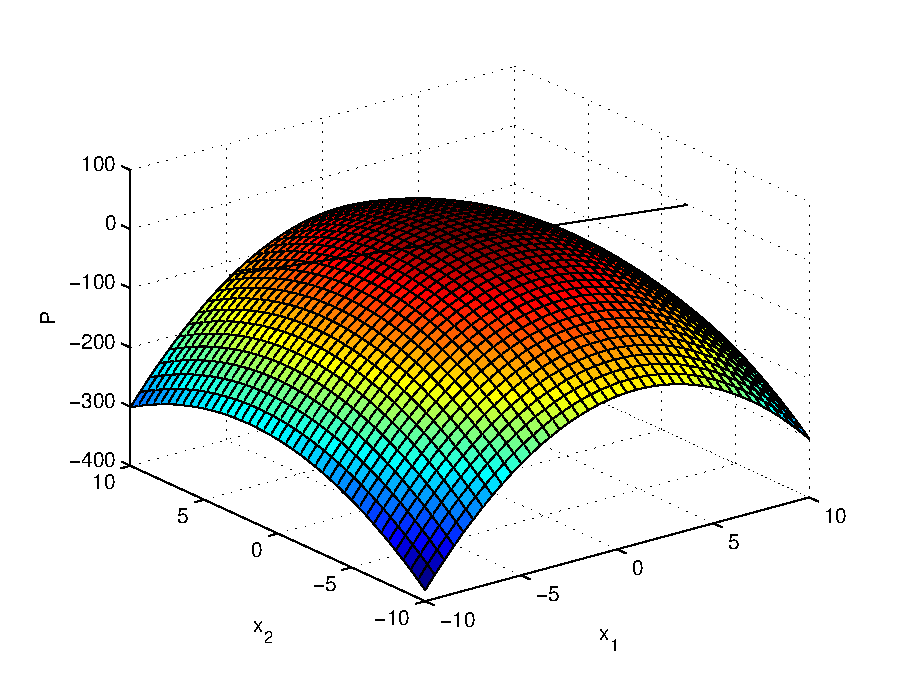
\includegraphics[keepaspectratio=true,width=0.4\linewidth]{MATLAB/optimizechap/lagran1/lagexam1.eps}}
\subfigure[Convex problem]{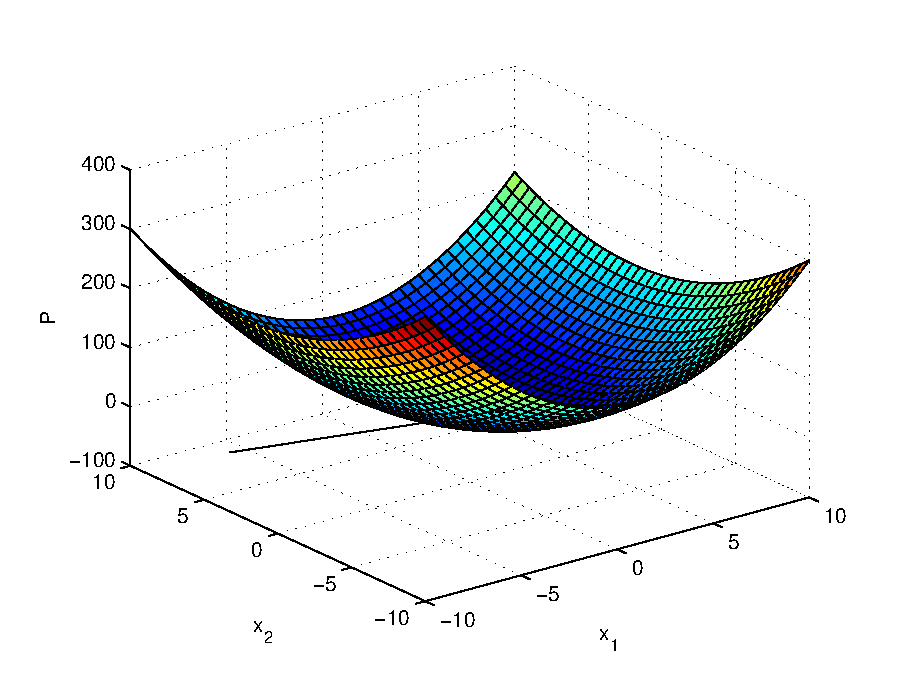
\includegraphics[keepaspectratio=true,width=0.4\linewidth]{MATLAB/optimizechap/lagran1/lagexam2.eps}}
%\caption{Concave Problem : $5-(x_{1}-2)^{2}-2(x_{2}-1)^{2}$}
\label{fig:10-1}
\caption{Convex and concave problem}
\end{figure}

여러개의 구속조건을 갖는 최적화 방식을 일반화 시키면
\begin{equation*}
\begin{aligned}
P : & \underset{x}{\text{maximize}}
& & f(x)\\
& \text{subject to}
& & g_{1}(x)=b_{1}\\
& & & g_{2}(x)=b_{1}\\
& & & \vdots\\
& & & g_{m}(x)=b_{m}\\
\end{aligned}
\end{equation*}
라그랑지안(Lagrangian)을 사용한 해는 다음 식으로 찾을 수 있다.
\begin{equation}
L(x,\lambda)=f(x)+\sum_{i=1}^{m}\lambda_{i}\left(b_{i}-g_{i}(x)\right)
\end{equation}
여기서, $\lambda_{i}$는 $i$번째 구속조건에 관련한 가중치(가격)으로 생각할 수 있다.
\begin{theorem}[Lagrangian multiplier]\label{theo:10-1}
최적화 문제 $P$를 만족시키는 $x^{*}$에 대하여 $x^{*}$와 $\lambda^{*}$가 존재 하고,
$x^{*}=\left(x_{1}^{*},x_{2}^{*},\cdots,x_{n}^{*}\right)$를 함수 $f(x)$를 구속조건 $g_{i}(x)=b_{i},\text{ for }i=1,2,\cdots,m$을 만족시키면서 최대화(maximizes)시키거나 최소화(minimizes)시키는 값을 가지는 벡터로 가정하면,
\begin{itemize}
\item[($i$)] 벡터 $\nabla g_{1}(x^{*}),\nabla g_{2}(x^{*}),\cdots,\nabla g_{m}(x^{*})$가 모두 선형적으로 독립이거나,
\item[($ii$)] $\nabla L(x^{*},\lambda^{*})=0$을 만족시키는 벡터 $\lambda^{*}=\left(\lambda_{1}^{*},\lambda_{2}^{*},\cdots,\lambda_{m}^{*}\right)$가 존재한다.
\end{itemize}
여기서 $\nabla$연산자(Nabla-operator)는 벡터의 편미분 연산자로 다음 식처럼 쓰인다.
\begin{equation}
\nabla = \left(\frac{\partial}{\partial x_{1}},\cdots,\frac{\partial}{\partial x_{n}}\right)
\end{equation}
즉, 위의 라그랑지안 정리는 다음식처럼 쓸 수 있다.
\begin{align}
\frac{\partial L}{\partial x_{1}}\left(x^{*},\lambda^{*}\right)=\frac{\partial L}{\partial x_{2}}\left(x^{*},\lambda^{*}\right)=\cdots=\frac{\partial L}{\partial x_{n}}\left(x^{*},\lambda^{*}\right)=0\\
\frac{\partial L}{\partial \lambda_{1}}\left(x^{*},\lambda^{*}\right)=\frac{\partial L}{\partial \lambda_{2}}\left(x^{*},\lambda^{*}\right)=\cdots=\frac{\partial L}{\partial \lambda_{m}}\left(x^{*},\lambda^{*}\right)=0
\end{align}
\end{theorem}

\subsection{등식과 부등식 구속조건 (Equality and Inequality Constraints)}
등식 구속조건과 부등식 구속조건이 포함된 함수의 최적화는 어떻게 두가지의 조건들을 사용할 수 있느냐에 달려있다. 일반화된 다음 식을 보자.
\begin{equation*}
\begin{aligned}
P : & \underset{x}{\text{maximize}}
& & f(x)\\
& \text{subject to}
& & g_{1}(x)=b_{1}\\
& & & \vdots\\
& & & g_{m}(x)=b_{m}\\
& & & h_{1}(x)\leq d_{1}\\
& & & \vdots\\
& & & h_{p}(x)\leq d_{p}\\
\end{aligned}
\end{equation*}
만약 이 조건이 아닌 $\geq$조건의 경우 $\leq$를 만들어주기 위해 양변에 $-1$을 곱하여 위와 동일한 조건을 만들어준다. 또한 같은 방식으로 최소값 문제는 최대값 문제로 변형할 수 있다.
이 때 라그랑지안은
\begin{equation}
L(x,\lambda,\mu)=f(x)+\sum_{i=1}^{m}\lambda_{i}\left(b_{i}-g_{i}(x)\right)+\sum_{j=1}^{p}\mu_{j}\left(d_{i}-h_{j}(x)\right)
\end{equation}
정리~\ref{theo:10-1}와 유사하게 다음과 같이 정리한다.
$x^{*}=\left(x_{1}^{*},x_{2}^{*},\cdots,x_{n}^{*}\right)$를 함수 $f(x)$를 구속조건 $g_{i}(x)=b_{i},\text{ for }i=1,2,\cdots,m$과 $h_{j}(x)\leq d_{j},\text{ for }j=1,2,\cdots,p$을 만족시키면서 최대화(maximizes)시키는 값을 가지는 벡터로 가정하면,
\begin{itemize}
\item[($i$)] 벡터 $\nabla g_{1}(x^{*}),\cdots,\nabla g_{m}(x^{*})$와 $\nabla h_{1}(x^{*}),\cdots,\nabla h_{p}(x^{*})$가 모두 선형적으로 독립이거나,
\item[($ii$)] 아래의 식을 만족시키는 벡터 $\lambda^{*}=\left(\lambda_{1}^{*},\cdots,\lambda_{m}^{*}\right)$와 $\mu^{*}=\left(\mu_{1}^{*},\cdots,\mu_{p}^{*}\right)$가 존재한다.
\end{itemize}
\begin{align*}
\nabla f(x^{*})-\sum_{i=1}^{m}\lambda_{i}^{*}\nabla g_{i}(x^{*})-\sum_{j=1}^{p}\mu_{j}^{*}\nabla h_{j}(x^{*})&=0\\
\mu_{j}^{*}\left(d_{j}-h_{j}(x^{*})\right)&=0\text{ (Complementarity)}\\
\mu_{j}^{*}&\geq0
\end{align*}
일반적으로 부등식조건이 포함된 해를 구하기 위해서는 우리는 $\mu_{j}^{*}$가 0이 되야하는 조건과 $d_{j}-h_{j}(x_{*})=0$이 되는 상보성(complementarity)조건을 검토해야한다. 이 조건에 만족하는 여러가지 경우의 수에 근거하여 우리는 적절한 하나의 해 혹은 후보해들을 선택해야한다. 만약 최적의 해가 존재한다면, 하나의 해 아니면 후보해들이 그 답이 될 것이다. 위의 조건들은 Kuhn-Tucker(혹은 Karush-Kuhn-Tucker)조건이라고 말한다. KKT조건에서 말하는 것은 최적의 해 $x^{*}$는 부등식 조건에서 꽉 찬 조건이거나 그렇지 않은 경우의 수가 있다. 즉, 부등식 조건에 꽉 찬 조건이 아닌 경우는 무시할 수 있다(해당 경우엔 $\mu_{j}^{*}=0$이 되므로). 그러나 부등식 조건에 꽉 찬 경우는 Lagrangian의 등식조건으로 생각할 수 있기 때문이다.
\begin{equation*}
\mu_{j}^{*}\left(d_{j}-h_{j}(x^{*})\right)=0\text{ (Complementarity)}
\end{equation*}
결국 이 식이 의미하는 것은 최적화 문제에서 부등식조건의 가중치 $\mu_{j}^{*}$를 0으로 잡거나, 구속조건을 꽉 채운 등식조건으로 인식하게 한다.
%\subsubsection{조건의 효용성(Sufficiency of conditions}
%KKT조건(Karush-Kuhn-Tucker conditions)은 적절한 최적해 $x^{*}$의 후보해를 제시해준다. 어떠한 경우에 최적의 충분조건을 
\\
\framebox{예제} \textbf{Complementarity}\\
\rule{\textwidth}{0.1pt}
\begin{equation*}
\begin{aligned}
& \underset{x}{\text{maximize}}& & x^{3}-3x\\
& \text{subject to}& & x\leq2\\
\end{aligned}
\end{equation*}
라그랑지안은
\begin{equation*}
L=x^{3}-3x+\mu(2-x)
\end{equation*}
풀면
\begin{align*}
\frac{\partial L}{\partial x}&=3x^{2}-3-\mu=0\\
x&\leq2\\
\mu(2-x)&=0\\
\mu&\geq0
\end{align*}
2가지의 상보성 조건이 존재한다.
\begin{itemize}
\item 만약 $\mu=0$의 경우에 $3x^{2}-3=0$이 되어 $x=\pm1$이 되고 $f(1)=-2$, $f(-1)=2$가 되기 때문에 해로 적합하다. 
\item 만약 $x=2$라면 $\mu=9$가 된다. 이때도 마찬가지로 $f(2)=2$가 되기 때문에 해로 적합하다.
\end{itemize}
따라서 최대값을 갖는 경우는 2가지의 해를 가지게 된다. $x=-1$과 $x=2$.
\\
\framebox{예제} \textbf{Standard form}\\
\rule{\textwidth}{0.1pt}
\begin{equation*}
\begin{aligned}
& \underset{x,y}{\text{minimize}}& & (x-2)^{2}+2(y-1)^{2}\\
& \text{subject to}& & x+4y\leq 3\\
& & & x\geq y\\
\end{aligned}
\end{equation*}
위의 식을 최대값을 갖는 형태와 표준형태로 변형하면,
\begin{equation*}
\begin{aligned}
& \underset{x,y}{\text{maximize}}& & -(x-2)^{2}-2(y-1)^{2}\\
& \text{subject to}& & x+4y\leq 3\\
& & & -x+y\leq0\\
\end{aligned}
\end{equation*}
라그랑지안은
\begin{equation*}
L(x,y,\mu_{1},\mu_{2})=-(x-2)^{2}-2(y-1)^{2}+\mu_{1}(3-x-4y)+\mu_{2}(0+x-y)
\end{equation*}
풀면 다음 조건이 된다.
\begin{align*}
\frac{\partial L}{\partial x}&=-2(x-2)-\mu_{1}+\mu_{2}=0\\
\frac{\partial L}{\partial y}&=-4(y-1)-4\mu_{1}-\mu_{2}=0\\
\frac{\partial L}{\partial \mu_{1}}&=\mu_{1}(3-x-4y)=0\\
\frac{\partial L}{\partial \mu_{2}}&=\mu_{1}(x-y)=0\\
x+4y&\leq3\\
-x+y&\leq0\\
\mu_{1},\mu_{2}&\geq0
\end{align*}
여기서 총 2개의 상보성 조건이 존재하기 때문에, 우리는 4가지의 경우를 체크해야한다.
\begin{itemize}
\item $\mu_{1}=0$, $\mu_{2}=0$의 경우 $x=2$, $y=1$이 되기 때문에 해로 부적합하다.
\item $\mu_{1}=0$, $x-y=0$의 경우 $x=4/3$, $y=4/3$, $\mu_{2}=-4/3$이 되기 때문에 해로 부적합하다.
\item $\mu_{2}=0$, $3-x-4y=0$의 경우 $x=5/3$, $y=1/3$, $\mu_{1}=2/3$이 되므로 해로 적합하다.
\item $3-x-4y=0$, $x-y=0$의 경우 $x=3/5$, $y=3/5$, $\mu_{1}=22/25$, $\mu_{2}=-48/25$가 되므로 해로 부적합하다.
\end{itemize}
따라서 최적해는 $x=5/3$, $y=1/3$임을 알 수 있다.
%\subsubsection{쿤-터커 정리(Kuhn-Tucker theroem)}
%부등식 조건이 포함된 최적화문제의 1계조건(First Order Condition)에 대한 정리이다. 위의 일반적인 최적화 문제에서 부등식 조건만 생각해보자.
%\begin{equation*}
%\begin{aligned}
%P : & \underset{x}{\text{maximize}}
%& & f(x)\\
%& \text{subject to}& & g_{1}(x)\leq b_{1}\\
%& & & g_{2}(x)\leq b_{2}\\
%& & & \vdots\\
%& & & g_{m}(x)=b_{m}\\
%& & & x_{j}\geq0, j=1,\cdots,n\\
%\end{aligned}
%\end{equation*}
%$(x_{1},x_{2},\cdots,x_{n})$이 원래 모델의 최적해라면, 다음과 같은 조건을 만족시키는 Lagrangian multiplier $\lambda$가 존재한다.
%\begin{align}
%\frac{\partial f}{\partial x_{j}}-\sum_{i=1}^{m}\frac{\partial g_{i}}{\partial x_{j}}&\leq 0, j=1,2,\cdots,n\\
%g_{i}(x_{1},x_{2},\cdots,x_{n})-b_{i}&\leq 0, i=1,2,\cdots,m\\
%x_{j}&\geq0, j=1,2,\cdots,n\\
%\lambda_{i}&\geq0, i=1,2,\cdots,m\\
%\end{align}
\subsection{선형계획모형 해법}
선형계획모형의 해를 구하는 해법으로 도해법(graphical solution)과 대수적 방법(algebraic method)이 있다. 도해법은 의사결정변수가 2개인 경우에 2차원 평면에서 적용될 수 있어 유용하지만, 3개이상인 경우 적용되는데 어려움이 발생하여 일반적인 해법이라고 보기 어렵다. 일반적으로 2개 이상의 변수에서 도해법이 유용한 경우는 고정된 조건에 의해 특성을 알아보려할 때 유용하다. 또한 최적해를 구하는 해법의 특성을 이해하는데에도 필요하다. 보통 변수가 2개를 초과하면 대수적인 방법으로 해를 구해야한다. 대표적인 대수적 방법으로는 Simplex법, 타원체해법(ellipsoid algorithm), 그리고 Karmarkar의 알고리즘이 있다. Simplex법은 1947년 George B, Danzig에 의하여, 타원체해법은 1979년 Khachian에 의하여, Karmarker의 알고리즘은 1984년 Karmarkar에 의하여 개발되었으며 내부점해법(interior-point algorithm)으로도 불린다. 타원체해법은 현재 거의 사용되지 않고 있고, 규모가 큰(large scale) 선형계획모형에 있어서는 근사치를 제고하는 내부점해법(interior-point method)이 Simplex법보다 복잡성 측면에서 우수한 것으로 알려져 있으나 일반적인 규모에서는 Simplex법이 효용성이 인정되어 아직도 널리 사용되고 있다. MATLAB Optimization Toolbox 패키지의 \texttt{linprog}의 함수에서도 규모를 분리하여 내부점해법과 Simplex법을 모두 차용하고 있다.\\
\framebox{문제} \textbf{LP문제 세우기}\\
\rule{\textwidth}{0.1pt}
다음의 문제는 화학공학, 혹은 석유공학분야에서 발생하는 문제이다. 그러나 유한한 자원을 가지고 제품을 생산하는 모든 공학분야에도 적용할 수 있다.\\
가스를 정제하는 공장이 매주 일정한 양의 원료가스를 받는다고 가정한다. 원료가스는 난방용 가스로 사용되는 보통 및 우수 품질의 두 가지 등급으로 정제된다. 이러한 등급들의 가스는 매우 수요가 높으며(항상 잘 팔림), 회사에 각각 다른 이윤을 가져다 준다. 그렇지만 이것들의 생산은 시간과 공장 내의 저장이라는 구속조건을 갖는다. 예를 들면 한 번에 한 개 등급의 제품만이 생산되며, 시설물은 단지 주당 80시간만 사용된다. 또한 각각의 제품들에 대하여 공장 내 보관장소의 제약이 따른다. 이러한 모든 인자들을 아래의 표로 정리되어 있다.
\begin{table}[!hbt]
\centering
\begin{tabular}{c|c|c|c}
\hline\hline
&\multicolumn{2}{c|}{Product}&\\
\cline{2-3}
Resource&Regular&Premium&Resource Availability\\
\hline
Raw gas& $7m^{3}/\text{tonne}$ & $11m^{3}/\text{tonne}$ & $77m^{3}/\text{week}$\\
Production time& $10hr/\text{tonne}$ & $8hr/\text{tonne}$ & $80hr/\text{week}$\\
Storage& $9\text{tonnes}$ & $6\text{tonnes}$ & -\\
\hline
Profit& $150/\text{tonne}$ & $175/\text{tonne}$ & -\\
\hline\hline
\end{tabular}
\end{table}
\\위의 선형프로그래밍문제는 교재에서는 Simplex법을 기초로 설명하고 있다. 일단 이 서술형 문제에서 선형프로그래밍식으로 작성해보자.
공장을 가동하는 기술자는 이윤을 극대화하기 위하여 각각 얼마만큼의 가스들을 생산할지를 결정하여야 한다. 주당 생산되는 보통 등급과 우수 등급의 제품의 양을 각각 $x_{1}$과 $x_{2}$라고 한다면, 주당 전체 이윤은 다음과 같이 계산된다.
\begin{equation*}
\text{total profit per week}=150x_{1}+175x_{2}
\end{equation*}
구속조건들은 비슷한 방법으로 구할 수 있다. 예를 들면 전체 원료가스의 사용량은 다음과 같이 계산된다.
\begin{equation*}
\text{total gas used amount per week}=7x_{1}+11x_{2}
\end{equation*}
이 함계는 주당 가용한 양인 $77m^{3}/week$를 넘지 않아야한다. 따라서 구속조건은 다음 과 같이 표시된다.
\begin{equation*}
7x_{1}+11x_{2}\leq77
\end{equation*}
남은 구속조건들도 같은 방법으로 구해지며, 이를 종합하면 선형프로그래밍식은 다음과 같다.
\begin{equation*}
\begin{aligned}
& \underset{x_{1},x_{2}}{\text{maximize}}& & Z=150x_{1}+175x_{2}&\text{이윤의 극대화}\\
& \text{subject to}& & 7x_{1}+11x_{2}\leq 77&\text{재료의 구속조건}\\
& & & 10x_{1}+8x_{2}\leq 80&\text{시간의 구속조건}\\
& & & x_{1}\leq 9&\text{''보통등급''의 보관 구속조건}\\
& & & x_{2}\leq 6&\text{''우수등급''의 보관 구속조건}\\
& & & x_{1},x_{2}\geq 0&\text{양수의 구속조건}\\
\end{aligned}
\end{equation*}
도해법으로 해를 구하면
\begin{figure}[!hbpt]
\centering
\subfigure[$7x_{1}+11x_{2}\leq 77$]{\includegraphics[keepaspectratio=true,width=0.4\textwidth]{MATLAB/optimizechap/lagran1/lin1.eps}}
\subfigure[$10x_{1}+8x_{2}\leq 80$]{\includegraphics[keepaspectratio=true,width=0.4\textwidth]{MATLAB/optimizechap/lagran1/lin2.eps}}
\subfigure[$x_{2}\leq 6$]{\includegraphics[keepaspectratio=true,width=0.4\textwidth]{MATLAB/optimizechap/lagran1/lin3.eps}}
\subfigure[$x_{1}\leq 9$]{\includegraphics[keepaspectratio=true,width=0.4\textwidth]{MATLAB/optimizechap/lagran1/lin4.eps}}
\subfigure[$x_{1},x_{2}\geq 0$]{\includegraphics[keepaspectratio=true,width=0.4\textwidth]{MATLAB/optimizechap/lagran1/lin6.eps}}
\subfigure[$Z=150x_{1}+175x_{2}$]{\includegraphics[keepaspectratio=true,width=0.4\textwidth]{MATLAB/optimizechap/lagran1/lin7.eps}}
\caption{Graphical solution}
\label{fig:10-2}
\end{figure}
\clearpage
\subsection{패키지를 사용한 최적화\\(MATLAB Optimization Toolbox Functions)}\label{sec:optoolbox}
다음 테이블은 MATLAB에서 사용할 수 있는 최적화 함수들을 나타낸다. 이 함수들은 최적화 툴박스에서 사용되어지지만 근을 구하거나, 최소화, 그리고 여러개의 목적함수를 둔 최적화 그리고 회귀분석에 이용될 수 있다.
%\subsubsection{Minimization Problems}
%\def\arraystretch{1.7}
\begin{table}[!hbt]
\centering
\begin{tabular}{l|M|l}
\hline\hline
Type&\text{Formulation}&Solver\tabularnewline\hline\hline
Scalar minimization&\begin{array}{cccc} & \underset{x}{\text{min}}&&f(x)\\&\text{subject to}&&l<x<u, (x\text{ is scalar})\end{array}&\texttt{fminbnd()}\tabularnewline\hline

Unconstrained minimization&\begin{array}{cccc} & \underset{x}{\text{min}}&&f(x)\\&\text{subject to}&&(none)\end{array}&\texttt{fminunc()},\texttt{fminsearch()}\tabularnewline\hline

Linear programming&\begin{array}{cccc} & \underset{x}{\text{min}}&&\mathbf{f}^{\top}\mathbf{x}\\&\text{subject to}&&\mathbf{Ax}\leq \mathbf{b}, \mathbf{A}_{eq}\mathbf{x}=\mathbf{b}_{eq},l\leq x\leq u\end{array}&\texttt{linprog()}\tabularnewline\hline

Quadratic programming&\begin{array}{cccc} & \underset{x}{\text{min}}&&\frac{1}{2}\mathbf{x}^{\top}\mathbf{Hx}+\mathbf{c}^{\top}\mathbf{x}\\&\text{subject to}&&\mathbf{Ax}\leq \mathbf{b}, \mathbf{A}_{eq}\mathbf{x}=\mathbf{b}_{eq},l\leq x\leq u\end{array}&\texttt{quadprog()}\tabularnewline\hline

Constrained minimization&\begin{array}{cccc} & \underset{\mathbf{x}}{\text{min}}&&f(\mathbf{x})\\&\text{subject to}&&c(x)\leq0,c_{eq}(x)=0,\\&&&\mathbf{Ax}\leq \mathbf{b}, \mathbf{A}_{eq}\mathbf{x}=\mathbf{b}_{eq},l\leq x\leq u\end{array}&\texttt{fmincon()}\tabularnewline\hline\hline

\end{tabular}
\end{table}
\subsubsection{Linear programming \texttt{lingprog()}}
MATLAB함수의 \texttt{lingprog()}는 선형계획법의 최적해를 구해준다. \texttt{linprog()}함수가 사용하는 알고리즘은 옵션에 선언해 주지 않는 이상 Large scale linear programming과 Medium scale linear programming 으로 자동선택되어 사용되어진다. 디폴트 옵션으로 사용되어지는 Large scale LP는 Mehrotra's predictor-corrector 알고리즘\footnote{Mehrotra, S., "On the Implementation of a Primal-Dual Interior Point Method," SIAM Journal on Optimization, Vol. 2, pp 575–601, 1992.}의 변형인 primal-dual interior-point method를 사용한 LIPSOL\footnote{Zhang, Y., "Solving Large-Scale Linear Programs by Interior-Point Methods Under the MATLAB Environment," Department of Mathematics and Statistics, University of Maryland, Baltimore County, Baltimore, MD, Technical Report TR96-01, July, 1995.}법을 사용한다. Medium scale LP는 1947년 George Dantzig\footnote{George B. Dantzig, "Programming of Interdependent Activities: II Mathematical Model" Econometrica Vol. 17, No. 3/4, pp. 200-211, 1949.}가 개발한 Simplex법(Simplex method)를 사용한다.
\begin{equation*}
\begin{aligned}
& \underset{\mathbf{x}}{\text{minimize}}& & \mathbf{f}^{\top}\\
& \text{subject to}& & \mathbf{A}\cdot\mathbf{x}\leq\mathbf{b}\\
& & & \mathbf{A}_{eq}\cdot\mathbf{x}=\mathbf{b}_{eq}\\
& & & \mathbf{L}_{b}\leq\mathbf{x}\leq\mathbf{U}_{b}\\
\end{aligned}
\end{equation*}
위의 수식은 MATLAB에서 사용할 수 있는 형태로 표현하기 위해, 행렬형태를 사용한다. \\
\texttt{[x,fval,exitflag,output,lambda] = }\textbf{linprog}\texttt{(f,A,b,Aeq,beq,lb,ub,x0,options)}
\begin{table}[!hbt]
\centering
\begin{tabular}{l|l}
\hline\hline
\texttt{f}& Linear objective function vector \texttt{f}\\\hline
\texttt{Aineq}& Matrix for linear inequality constraints\\\hline
\texttt{bineq}& Vector for linear inequality constraints\\\hline
\texttt{Aeq}& Matrix for linear equality constraints\\\hline
\texttt{beq}& Vector for linear equality constraints\\\hline
\texttt{lb}& Vector of lower boundsubVector of upper bounds\\\hline
\texttt{x0}& Initial point for \texttt{x}, active set algorithm only\\\hline
\texttt{solver}& \texttt{'linprog'}\\\hline
\texttt{options}& Options structure created with \texttt{optimset()}\\
\hline\hline
\end{tabular}
\caption{Input Arguments}
\end{table}
앞서 언급한대로 MATLAB프로그램을 수행하면, Large-scale optimization 방식으로 선형프로그래밍의 최적해를 구한다.
\lstinputlisting[language=Matlab, caption= 가스정제공장 수익극대화의 최적해]{MATLAB/optimizechap/lagran1/linprogramex1.m} 

\clearpage
\part{곡선적합\\(Curve Fitting)}
공학에서 측정된 데이터를 사용하여 물리적 모델 혹은 요소들을 추정하는 경우가 대부분이다. 이 때 데이터는 연속적이기 보다는 이산적인 값으로 주어지는 경우가 많고, 이산적인 값 사이에 있는 임의의 점에서의 값을 추정해야 하는 경우가 있다. 또한 복잡한 함수를 단순화된 모델로 만들어야 하는 경우도 있다. 이 경우 임의의 수의 특정한 점들에서 그 함수값을 추적하고, 이들 계산값과 보간법을 이용하여 보다 간단한 형태의 함수로 표현할 수 있다. 이와 같은 응용들을 모두 일컬어 곡선적합(curve fitting)이라고 한다.

곡선적합은 데이터와 관련된 오차의 크기에 따라서 접근방법이 두 가지로 구별된다. 첫 번째 방법은 데이터가 상당한 크기의 오차 또는 "노이즈(noise)"를 내포하고 있을 경우로 데이터의 일반적인 경향을 나타내는 하나의 곡선을 유도해 내는 방법이다. 이 경우, 각각의 데이터값은 정확하지 않을 수 있기 때문에 유도되는 곡선이 모든 데이터점들을 통과하도록 노력할 필요는 없으나, 유도되는 곡선은 각 데이터점들의 경향을 따르도록 결정하여야 한다. 이러한 방식으로 데이터의 경향을 적절하게 표현하는 한 가지 방법으로 최소제곱회귀분석(least-square regression)이 있다. 두번째 방법은 데이터값들이 상당히 정확하여 각각의 데이터점들을 직접 통과하는 하나의 곡선, 또는 일련의 곡선들을 매끄럽게 연결하는 방법이다. 이 경우의 데이터는 보통 도표에 있는 값들로서, 예를 들면 온도의 함수로 표현되는 물의 밀도에 대한 값, 또는 가스의 비열에 대한 값들을 말한다. 값이 알려진 두 점들 사이에 있는 임의의 점에서 함수값을 추정하는 방법을 보간법(interpolation)이라고 한다.

\begin{figure}[!hbpt]
\centering
\subfigure[최소제곱회귀분석]{\includegraphics[keepaspectratio=true,width=0.3\linewidth]{MATLAB/chap11/pt5-1a.eps}}
\subfigure[선형보간]{\includegraphics[keepaspectratio=true,width=0.3\linewidth]{MATLAB/chap11/pt5-1b.eps}}
\subfigure[곡선보간]{\includegraphics[keepaspectratio=true,width=0.3\linewidth]{MATLAB/chap11/pt5-1c.eps}}
\label{fig:pt5-1}
\caption{10개의 점들을 최적의 곡선으로 보간하는 세가지 방법}
\end{figure}

경제공학에서 이율도표나, 열역학에서의 증기표 그리고 토목공학에서 응력변형도 곡선등과 같이 도표화된 데이터로부터 중간값을 결정하는 방식을 경험하였다. 비록 널리 사영되는 공학적 물성치들이 대부분이 도표화 혹은 공식화되어 있음에도 불구하고 많은 물성치들은 이러한 편리한 형태로 얻을 수 없다. 자신이 직접 데이터를 측정하거나, 예측관계식을 개발하여야 하는 특별한 경우와 같이 새로운 분야가 종종 발생된다. 실험데이터를 보간할 때는 경향분석(trend analysis)이나 가상실험(hypothesis testing)과 같은 두 가지 형태의 응용문제와 마주치게 된다.

경향분석은 예측을 하기 위하여 데이터의 형(pattern)을 분석하는 과정을 나타낸다. 데이터가 높은 정확도로 측정된 경우 보간다항식을 이용할 수 있으나, 정확도가 높지 않은 데이터는 보편적으로 최소제곱회귀분석이 사용된다.

실험적 곡선적합의 두 번째의 공학적 적용은 가상실험이다. 이것은 현존하는 수학적 모델과 측정된 데이터를 비교하는 것이다. 만약 모델의 계수들을 알지 못한다면, 관측된 데이터에 최적으로 적합한 계수들을 결정하여야 한다. 한편, 만약 모델 계수의 추정값이 이미 확보된 경우에는 관측된 값과 모델의 예측값을 서로 비교하여 모델의 적합성을 검사하는 것이 필요할 것이다. 이 때 대안으로 제시되는 모델과 비교되어 실험적인 관측에 근거한 "최적"인 모델이 선택된다.

\section{최소제곱회귀분석\\(Lest Square Regression)}
\subsection{통계학 기초}
공학적 연구 과정에서 어떤 특정한 양을 여러번 측정하였다고 가정하자. 

\begin{table}[!hbt]
\centering
\begin{tabular}{c|c|c|c|c|c}
\hline\hline
6.495&6.595&6.615&6.635&6.485&6.555\\
6.665&6.505&6.435&6.625&6.715&6.655\\
6.755&6.625&6.715&6.575&6.655&6.605\\
6.565&6.515&6.555&6.395&6.775&6.685\\
\hline\hline
\end{tabular}
\caption{철 구조물의 열팽창계수[$\times 10^{-6}\text{in}/(\text{in}\cdot^{\circ}\text{F})$]측정}
\label{tab:pt5-1}
\end{table}

예로 표\ref{tab:pt5-1}는 철 구조물(steel structure)의 열팽창계수에 관한 24개의 측정된 값들을 나타내고 있다. 표에 있는 값들을 보면 데이터는 최소 6.395로부터 최대 6.775의 범위 내에서 제한된 분량의 정보만을 제공하고 있다. 적절한 통계법을 이용하여 데이터를 요약하는 것으로 데이터 집합의 특수한 성질에 관하여 보다 많은 정보를 제공할 수 있는 추가적인 관찰 결과를 얻을 수 있다. 이러한 분석적인 통계법들은 (1) 데이터 분포의 중심위치 (2) 데이터 집합의 분산 정도등을 나타내는데 주로 사용된다.

가장 보편적인 통계값은 산술평균(arithmetic mean)이다. 어떤 표본의 산술평균($\bar{y}$)은 다음과 같이 각각의 데이터값($y_{i}$)들을 합하고, 이것을 데이터점의 수($n$)으로 나눈 것으로 정의된다.
\begin{equation}\label{eq:pt5-1}
\bar{y}=\frac{\sum y_{i}}{n}
\end{equation}

여기서 합(이후의 모든 합)은 $i=1$부터 $n$까지를 나타낸다.
또한, 가장 보편적인 표본의 분포도는 다음과 같이 정의되는 평균을 중심으로 하는 표준편차(standard deviation, $s_{y}$)이다.
\begin{equation}\label{eq:pt5-2}
s_{y}=\sqrt{\frac{S_{t}}{n-1}}
\end{equation}
여기서 $S_{t}$는 데이터점들과 평균 사이의 잔차를 제곱한 총합을 말한다. 즉 $S_{t}$는 다음과 같다.
\begin{equation}\label{eq:pt5-3}
S_{t}=\sum\left(y_{i}-\bar{y}\right)^{2}
\end{equation}
따라서 만약 개별적인 측정값들이 평균값 주변에 넓게 퍼져 있다면 $S_{t}$(결과적으로는 $s_{y}$)의 값은 커질 것이다. 만약에 측정값들이 모여 있다면 표준편차는 줄어든다. 분포는 표준편차의 제곱으로 다음과 같이 나타낼 수 있으며, 이것을 분산(variance, $s_{y}^2$)이라고 한다.
\begin{equation}\label{eq:pt5-4}
s_{y}^{2}=\frac{\sum\left(y_{i}-\bar{y}\right)^{2}}{n-1}
\end{equation}
여기서 식(\ref{eq:pt5-2})와 식(\ref{eq:pt5-4})에 있는 분모가 $(n-1)$인데 이것을 자유도(degree of freedom)이라고 한다. 따라서 $S_{t}$와 $s_{y}$는 $(n-1)$자유도에 기초를 두고 있다.
데이터 분포를 수치화하는 데 이용되는 통계값으로는 분산계수(coefficient of variation; c.v.)가 있으며, 이것은 평균에 대한 표준편차의 비율이다. 이 값은 정규화된 분포도를 다음과 같이 백분율의 형태로 나타내고 있다.
\begin{equation}\label{eq:pt5-5}
\text{c.v.}=\frac{s_{y}}{\bar{y}}\times 100
\end{equation}
\subsubsection{정규분포}
데이터가 평균값 주위에 분포되어 있는 형태가 있다. 히스토그램(histogram)은 데이터의 분포에 대한 간단한 시각적 표현을 제공해 주며, 측정값을 구간별로 분류해서 구성하게 된다. 이때 측정단위는 수평축에 나타내고 각 구간의 발생 빈도는 수직축에 나타낸다. 만약 많은 수의 데이터를 갖고 있을 경우 이러한 히스토그램은 매끄러운 곡선으로 근사화될 수가 있다.
\begin{figure}[!hbpt]
\centering
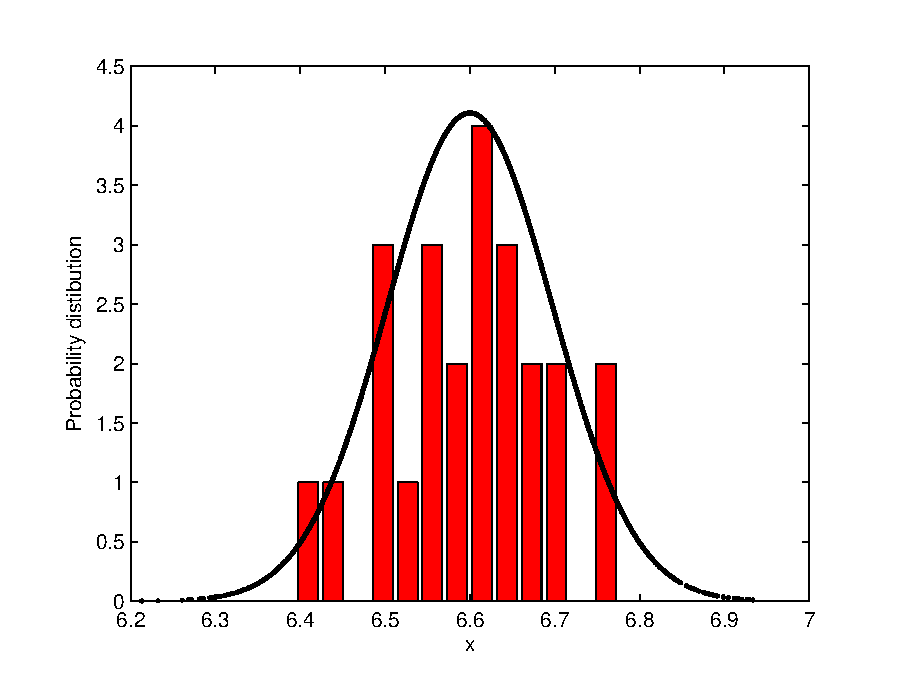
\includegraphics[keepaspectratio=true,width=0.6\linewidth]{MATLAB/chap11/dist.eps}
\label{fig:pt5-2}
\caption{정규분포}
\end{figure}
Figure~\ref{fig:pt5-2}에 나타낸 종 모양으로 된 대칭곡선은 이러한 근사화된 특성 곡선의 하나로써 정규분포(normal distribution)이라고 하며, 데이터점들의 수가 증가할 수록 히스토그램은 결국 이러한 정규분포에 접근하게 된다.

평균, 표준편차, 잔차의 제곱합 그리고 정규분포와 같은 개념들은 모두 공학문제와 큰 연관성을 갖고 있다. 매우 간단한 예로는 이들이 어떤 특정한 측정값에 대한 신뢰도를 정량화시키는데 사용될 수가 있다는 것이다. 만약 어떤 양이 정규적으로 분포되어 있다면 $\bar{y}-s_{y}$와 $\bar{y}+s_{y}$사이의 구간에는 전체 측정 개수의 약 68\%를 포함하게 된다. 같은 방식으로 아래의 식들과 같이 정량적인 방법으로 물리적인 양을 가늠할 수 있다.
\begin{align*}
\bar{y}-s_{y}\leq&\text{측정 개수의 }68\%\leq\bar{y}+s_{y}\\
\bar{y}-1.96s_{y}\leq&\text{측정 개수의 }95\%\leq\bar{y}+1.96s_{y}\\
\bar{y}-2.54s_{y}\leq&\text{측정 개수의 }99\%\leq\bar{y}+2.54s_{y}
\end{align*}
예를들어 Table~\ref{tab:pt5-1}에서와 같이 주어진 열팽창계수 데이터($\bar{y}=6.6$과 $s_{y}=0.097133$)에 대하여 우리는 약 95\%의 측정값들이 6.409619와 6.790381 사이에 존재한다고 할 수 있다. 만약에 어떤 사람이 7.35라는 값을 측정했다고 하면 우리는 그 측정값은 틀렸다고 의심하게 될 것이다. 이러한 측정값에 대한 신뢰도에 대한 평가는 다음절에서 다뤄진다.
\subsubsection{신뢰구간의 산출}
앞 절에서와 같이 통계의 주목적은 집단으로부터 제한적으로 추출된 표본을 이용하여 그 집단의 특성을 파악하는데 있다. 생산되는 모든 구조물용 강재의 열팽창계수를 측정한다는 것이 불가능함은 명백하다. Table~\ref{tab:pt5-1}와 같이 표본추출에 근거하여 전체 집단의 특성을 규명할 수가 있다.

제한된 표본으로부터 모르는 집단의 물성을 "추론"해야 하기 때문에 이러한 노력을 '통계적인 추론'이라고 한다. 통계적 추론의 결과는 보통 집단에 대한 인자들의 추정값으로 주어지기 때문에 이러한 과정을 '추정'이라고도 한다.

기호 $\bar{y}$ 및 $s_{y}$등은 표본의 평균 및 표준편차를 나타내고, 기호 $\mu$ 및 $\sigma$등은 집단의 평균 및 표준편차를 각각 나타낸다. 전자의 표현은 "산출(estimated)"된 평균 및 표준편차라고 하고, 후자의 표현은 종종 "참(true)"평균 및 표준편차라고 한다.

구간추정자(interval estimator)는 그 인자가 주어진 확률로 갖게 되는 값의 범위를 제시해 준다. 그러한 구간들은 한쪽이거나 양쪽인 것으로 설명될 수 있다. 한쪽 구간이라 함은 인자의 산출이 참값보다 작거나 또는 큰 신뢰도를 나타낸다. 반면에 양쪽 구간은 산출값이 항상 참값과 일치하게 되는 보다 일반적인 상황을 다루게 된다. 양쪽 구간이 보다 일반적이기 때문에 여기서는 이에 초점을 맞추어 설명한다.
양쪽 구간은 다음과 같이 기술 될 수 있다.
\begin{equation}
P\left\{L\leq\mu\leq U\right\}=1-\alpha
\end{equation}

\begin{figure}[!hbpt]
\centering
\includegraphics[keepaspectratio=true,width=0.6\linewidth]{MATLAB/chap11/norm.eps}
\label{fig:pt5-3}
\caption{양쪽 구간 신뢰도 범위}
\end{figure}
이것은 "$y$의 참평균 $\mu$가 $L$과 $U$ 사이의 구간에 놓일 수 있는 확률이 $(1-\alpha)$이다"라고 읽는다. 여기서 $\alpha$값을 유효수준(significant level)이라고 부르며, 따라서 신뢰구간 (confidence level)을 결정하는 문제는 $L$과 $U$를 구하는 것으로 축소된다. 필수조건은 아니지만 Figure~\ref{fig:pt5-3}과 같이 분포의 각 끝단 꼬리에 같은 크기로 $\alpha/2$씩 분포된 $\alpha$확률을 갖는 양쪽 구간을 관찰하는 것이 보편적이다.

$y$의 분포에 대한 참분산 $\sigma^2$을 알수 없지만 알고있다고 가정하면 표본의 평균 $\bar{y}$는 평균이 $\mu$이고 분산값이 $\sigma^2/n$인 정규분포로부터 얻어질 수가 있다. Figure~\ref{fig:pt5-3}에 설명된 문제에서 실제적인 평균 $\mu$를 모르고 있다. 그러므로 표본의 평균 $\bar{y}$와 관련해서 정규곡선이 정확하게 어디에 놓이게 되는지를 알지 못한다. 따라서 표준정규추정(standard normal estimate)로 새로운 값을 산출한다.
\begin{equation}\label{eq:pt5-6}
\bar{z}=\frac{\bar{y}-\mu}{\sigma/\sqrt{n}}
\end{equation}
이것은 $\bar{y}$와 $\mu$사이의 정규화된 거리를 나타낸다. 통계학적 이론에 의하면 이 값은 평균 0이고, 분산값이 1인 정규분포가 되어야 한다. 더욱이 $\bar{z}$가 Figure~\ref{fig:pt5-3}에서 면적표시가 되지 않은 영역에 떨어질 확률은 $(1-\alpha)$이어야 한다. 그러므로 $\alpha$의 확률로써 다음과 같은 표현이 가능하다.
\begin{align*}
\frac{\bar{y}-\mu}{\sigma/\sqrt{n}}&<-z_{\alpha/2}\\
\frac{\bar{y}-\mu}{\sigma/\sqrt{n}}&>z_{\alpha/2}
\end{align*}
$z_{\alpha/2}$는 표준정규 임의변수(standard normal random variable)이다. 이 값은 $(1-\alpha)$확률에 걸쳐 있으며, 평균을 전후해서 무차원화된 좌표축을 따라 측정된 거리를 나타낸다. 이 값은 각 상용프로그램으로도 구할 수 있다. 예를들어 $\alpha=0.05$ 즉 95\%의 확률에 걸치구간 $z_{\alpha/2}$는 약 1.96과 같다. 이런 결과는 확률 $(1-\alpha)$로써 다음과 같이 쓸 수 있다.
\begin{equation*}
L\leq\mu\leq U
\end{equation*}
여기서, $L$ 및 $U$는 각각 다음과 같이 정의된다.
\begin{align*}
L&=\bar{y}-\frac{\sigma}{\sqrt{n}}z_{\alpha/2}\\
U&=\bar{y}+\frac{\sigma}{\sqrt{n}}z_{\alpha/2}
\end{align*}
\subsection{선형회귀분석}
최소제곱 근사의 간단한 방법으로 관측치에 직선으로 적합시키는 것이다.
\begin{equation}\label{eq:15-1}
y=a_{0}+a_{1}x+e
\end{equation}
여기서, $a_{0}$는 절편(intercept), $a_{1}$는 기울기(slope)그리고 $e$는 관측값과 모델값의 차이로 오차(error)이다. 오차는 식(\ref{eq:15-1})를 변형하여
\begin{equation}
e=y-a_{0}-a_{1}x
\end{equation}
\subsubsection{최적적합을 위한 조건}
(1) 데이터를 통과하는 최적의 직선(best fit)을 구하는 방법은 모든 주어진 데이터에 대한 오차의 합을 최소화 시키는 것이다.
\begin{equation}\label{eq:15-2a}
\sum_{i=1}^{n}e_{i}=\sum_{i=1}^{n}(y_{i}-a_{0}-a_{1}x_{i})
\end{equation}
\framebox{문제점?}\\
(2) 오차의 절대값의 합을 최소화 하는 방법
\begin{equation}\label{eq:15-2b}
\sum_{i=1}^{n}\left|e_{i}\right|=\sum_{i=1}^{n}\left|y_{i}-a_{0}-a_{1}x_{i}\right|
\end{equation}
\framebox{문제점?}\\
(3) 최소-최대(minimax) 판별조건은 직선으로부터 떨어진 각 점들의 최대 변위가 최소가 되도록 선택하는 것이다.

위에서 언급한 방법들의 단점을 극복하기 위하여 측정된 $y$와 선형 모델을 이용하여 계산된 $y$사이의 잔차에 대한 제곱의 합을 최소화하는 방법이 고안됨.
\begin{align}
S_{r}&=\sum_{i=1}^{n}e_{i}^2\nonumber\\
&=\sum_{i=1}^{n}\left(y_{i,measured}-y_{i,model}\right)^2\nonumber\\
&=\sum_{i=1}^{n}\left(y_{i}-a_{0}-a_{1}x_{i}\right)^2\label{eq:15-3}
\end{align}
\subsubsection{직선의 최소제곱적합}
$a_{0}$와 $a_{1}$의 값을 결정하기 위하여 식(\ref{eq:15-3})은 각각의 계수에 대하여 편미분을 취한다.
\begin{align*}
\frac{\partial S_{r}}{\partial a_{0}}&=-2\sum\left(y_{i}-a_{0}-a_{1}x_{i}\right)\\
\frac{\partial S_{r}}{\partial a_{1}}&=-2\sum\left[\left(y_{i}-a_{0}-a_{1}x_{i}\right)x_{i}\right]\\
\sum y_{i}-\sum a_{0}-\sum a_{1}x_{i}&=0\\
\sum y_{i}x_{i}-\sum a_{0}x_{i}-\sum a_{1}x_{i}^{2}&=0
\end{align*}
$\sum a_{0}=na_{0}$이므로 이 식은 $a_{0}$과 $a_{1}$에 대한 2원 1차 연립방정식으로 주어진다.
\begin{align}
na_{0}+\left(\sum x_{i}\right)a_{1}&=\sum y_{i}\label{eq:15-4}\\
\left(\sum x_{i}\right)a_{0}+\left(\sum x_{i}^{2} \right)a_{1}&=\sum x_{i}y_{i}
\end{align}
이들을 정규 방정식(normal equation)이라고 한다. 이들을 연립방정식으로 풀면 $a_{1}$은 다음과 같이 된다.
\begin{equation}
a_{1}=\frac{n\sum x_{i}y_{i}-\sum x_{i}\sum y_{i}}{n\sum x_{i}^{2}-\left(\sum x_{i}\right)^{2}}
\end{equation}
이 결과를 식(\ref{eq:15-4})에 대입해서 $a_{0}$를 구하면
\begin{equation}
a_{0}=\bar{y}-a_{1}\bar{x}
\end{equation}
여기서 $\bar{y}$와 $\bar{x}$는 각각 $y$와 $x$의 평균이다.
\subsubsection{선형회귀분석 오차의 정량화}
최소제곱법으로 얻은 직선은 점들의 경향을 나타내는 "최적"의 유일한 직선이라 할 수 있다. 잔차들이 계산되는 방식을 자세히 분석해보면 보간법의 여러 다른 성질들을 발견할 수 있다. 식(\ref{eq:15-3})에서 정의된 제곱합을 상기해보면
\begin{equation}\label{eq:15-8}
S_{r}=\sum_{i=1}^{n}e_{i}^{2}=\sum_{i=1}^{n}\left(y_{i}-a_{0}-a_{1}x_{i}\right)^{2}
\end{equation}
여기서 식(\ref{eq:pt5-3})과 식(\ref{eq:15-8})이 유사함을 보인다. 즉 (1) 데이터와 직선과의 차이는 데이터의 전체 범위에 걸쳐서 유사한 크기를 갖고, (2) 직선을 중심으로 한 데이터점들의 분포는 정규분포를 이룬다. 만약 이들 판별조건이 만족된다면 최소제곱회귀분석은 $a_{0}$과 $a_{1}$를 구하는 가장 좋은방법이라고 할 수 있다.(Draper and Smith, 1981). 이것을 "최대우도법칙(maximum likelihood principle)"이라 한다.
회귀분석직선에 대한 표준편차는 다음과 같이 결정된다.
\begin{equation}\label{eq:15-9}
s_{y/x}=\sqrt{\frac{S_{r}}{n-2}}
\end{equation}
식(\ref{eq:pt5-3})의 데이터의 표준편차와 오차의 제곱합 식(\ref{eq:15-8})을 이용하여 상대적인 오차로 정규화하면
\begin{equation}\label{eq:15-10}
r^{2}=\frac{S_{t}-S_{r}}{S_{t}}
\end{equation}
여기서, $r^{2}$를 결정계수(coefficient of determination), $r$을 상관계수(correlation coefficient)라 한다. $S_{r}=0$, $r=r^{2}=1$인 경우, 완전한 적합이므로 데이터는 회귀분석직선에 의하여 100\%만족한다. 컴퓨터 계산을 위해 식(\ref{eq:15-10})를 다음 식과 같이 사용하는 것이 편리하다.
\begin{equation}
r=\frac{n\sum x_{i}y_{i}-\left(\sum x_{i}\right)\left(\sum y_{i}\right)}{\sqrt{n\sum x_{i}^{2}-\left(\sum x_{i}\right)}\sqrt{n\sum y_{i}^{2} -\left(\sum y_{i}\right)^2}}
\end{equation}

\begin{algorithm}

\begin{algorithmic}
\Function{regression}{$x$,$y$,$n$,$a_1$,$a_0$,$s_{y/x}$,$r^2$}
\State $sumx=0$\; $sumxy=0$\; $st=0$\;
\State $sumy=0$\; $sumx2=0$\; $sr=0$\;
\For{$i=1$,$n$}
 \State $sumx=sumx+x_{i}$\;
 \State $sumy=sumy+y_{i}$\;
 \State $sumxy=symxy+x_{i}*y_{i}$\;
 \State $sumx2=sumx2+x_{i}*x_{i}$\;
\EndFor
\State $x_{m}=sumx/n$\;
\State $y_{m}=sumy/n$\;
\State $a_{1}=(n*sumxy-sumx*sumy)/(n*sumx2-sumx*sumx)$\;
\State $a_{0}=y_{m}-a_{1}*x_{m}$\;
\For{$i=1$,$n$}
 \State $S_{t}=S_{t}+(y_{i}-y_{m})^{2}$\;
 \State $S_{r}=S_{r}+(y_{i}-a_{1}x_{i}-a_{0})^{2}$\;
\EndFor
\State $s_{y/x}=\sqrt{S_{r}/(n-2)}$\;
\State $r^{2}=(S_{t}-S_{r})/S_{t}$\;
\State \Return $a_{1}$, $a_{0}$, $s_{y/x}$, $r^2$
\EndFunction
\end{algorithmic}
\caption{선형회귀분석 알고리즘}
\end{algorithm}
%\framebox{예제} \textbf{Newton-Raphson법 예제 ($\sqrt{2}$ 찾기)}\\
%
%\begin{equation}\label{eq:e15-1}
%v(t)=\frac{gm}{c}\left(1-e^{(-c/m)t}\right)
%\end{equation}
%
%\begin{equation}\label{eq:e15-3-1}
%v(t)=\frac{gm}{c}\left(\frac{t}{3.75+t}\right)
%\end{equation}
%
%\begin{table}[!hbt]
%\centering
%\begin{tabular}{c|c|c|c}
%\hline\hline
%&Measured $v$&Model-calculated&Model-calculated\\
%&$m/s$&$m/s$ [Eq.\ref{eq:e15-1}]&$m/s$ [Eq.\ref{eq:e15-3-1}]\\
%Time (s)&(a)&(b)&(c)\\
%\hline
%1&10.00&8.953&11.240\\
%2&16.30&16.405&18.520\\
%3&23.00&22.607&23.729\\
%4&27.50&27.769&27.556\\
%5&31.00&32.065&30.509\\
%6&35.60&35.641&32.855\\
%7&39.00&38.617&34.766\\
%8&41.50&41.095&36.351\\
%9&42.90&43.156&37.687\\
%10&45.00&44.872&38.829\\
%11&46.00&46.301&39.816\\
%12&45.50&47.490&40.678\\
%13&46.00&48.479&41.437\\
%14&49.00&49.303&42.110\\
%15&50.00&49.988&42.712\\
%\hline\hline
%\end{tabular}
%\caption{낙하하는 낙하산병에 대한 측정 및 계산 속도값들}
%\label{tab:pt5-1}
%\end{table}

\subsubsection{비선형 관계식의 선형화}
선형식으로 회귀분석 할 수 있는 비선형 방정식의 형태는 다음과 같은 지수모델로 변형할 수 있다.
\begin{equation}\label{eq:15-12}
y=\alpha_{1}e^{\beta_{1}x}
\end{equation}
여기서 $\alpha_{1}$, $\beta_{1}$은 상수이다. 이 모델은 공학의 여러분야에서 증가하는 양($\beta_{1}>0$), 또는 감소하는 양($\beta_{1}<0$)이 그 자신의 크기에 직접 비례하는 특성을 나타내는 모델이다. 예로 인구 증가모델, 또는 바사능 감소등이다. 또한 멱방정식형태를 예를 들 수 있다.
\begin{equation}\label{eq:15-13}
y=\alpha_{2}x^{\beta_{2}}
\end{equation}
여기서 $\alpha_{2}$, $\beta_{2}$은 상수이다. 또한 포화성장률 방정식(saturation-growth-rate equation)이 있다.
\begin{equation}\label{eq:15-14}
y=\alpha_{3}\frac{x}{\beta_{3}+x}
\end{equation}
여기서 $\alpha_{3}$, $\beta_{3}$은 상수이다. 이 모델은 제한된 조건하의 인구 성장모델이나 $x$가 증가함에 따라 성장이 정지 즉, 포화상태에 이르는 비선형관계식을 나타내고 있다. 이러한 방정식모델은 간단한 조작으로 선형화가 가능하기 때문에 단순 선형회귀분석으로 보간식을 구할 수 있다. 예를들어 식(\ref{eq:15-12})의 양반여 자연로그를 취하면,
\begin{align}
\ln y&=\ln\alpha_{1}+\beta_{1}x\ln e\nonumber\\
&=\ln\alpha_{1}+\beta_{1}x\label{eq:15-15}
\end{align}
따라서 $x$에 대한 $\ln y$의 그림은 $\beta_{1}$인 기울기와 $\ln \alpha_{1}$인 절편을 갖는다. 마찬가지로 식(\ref{eq:15-13})은 양변에 상용로그를 취해 선형화할 수 있다.
\begin{equation}\label{eq:15-16}
\log y=\beta_{2}\log x+\log \alpha_{2}
\end{equation}
식(\ref{eq:15-14})는 역수를 취하여 다음과 같이 선형화될 수 있다.
\begin{equation}\label{eq:15-17}
\frac{1}{y}=\frac{\beta_{3}}{\alpha_{3}}\frac{1}{x}+\frac{1}{\alpha_{3}}
\end{equation}
\framebox{예제} \textbf{멱 방정식의 선형화}\\
데이터의 $\log$변환을 이용하여 Table~\ref{tab:15-3}에 있는 데이터를 식(\ref{eq:15-13})으로 나타내어라.

\begin{table}[!hbt]
\centering
\begin{tabular}{c|l|l|l}
\hline\hline
$x$&$y$&$\log x$&$\log y$\\
\hline
1&0.5&0&-0.301\\
2&1.7&0.301&0.226\\
3&3.4&0.477&0.534\\
4&5.7&0.602&0.753\\
5&8.4&0.699&0.922\\
\hline\hline
\end{tabular}
\caption{멱방정식으로 적합되는 데이터}
\label{tab:15-3}
\end{table}

\subsubsection{다항식 회귀분석}
2차다항식의 모델 방정식
\begin{equation}
y=a_{0}+a_{1}x+a_{2}x^2+e
\end{equation}
잔차의 제곱합은 다음식과 같다.
\begin{equation}
S_{r}=\sum_{i=1}^{n}\left(y_{i}-a_{0}-a_{1}x_{i}-a_{2}x_{i}^{2}\right)^{2}
\end{equation}
각 미지계수에 대해 편미분을 수행하면,
\begin{align*}
\frac{\partial S_{r}}{\partial a_{0}}&=-2\sum\left(y_{i}-a_{0}-a_{1}x_{i}-a_{2}x_{i}^{2}\right)\\
\frac{\partial S_{r}}{\partial a_{1}}&=-2\sum x_{i}\left(y_{i}-a_{0}-a_{1}x_{i}-a_{2}x_{i}^{2}\right)\\
\frac{\partial S_{r}}{\partial a_{2}}&=-2\sum x_{i}^{2}\left(y_{i}-a_{0}-a_{1}x_{i}-a_{2}x_{i}^{2}\right)
\end{align*}
$S_{r}$이 최소값을 갖는 경우 값을 0으로 두고 정규방정식으로 정리할 수 있다.
\begin{align*}
na_{0}+\left(\sum x_{i}\right)a_{1}+\left(\sum x_{i}^{2}\right)a_{2}&=\sum y_{i}\\
\left(\sum x_{i}\right)a_{0}+\left(\sum x_{i}^{2}\right)a_{1}+\left(\sum x_{i}^{3}\right)a_{2}&=\sum x_{i}y_{i}\\
\left(\sum x_{i}^{2}\right)a_{0}+\left(\sum x_{i}^{3}\right)a_{1}+\left(\sum x_{i}^{4}\right)a_{2}&=\sum x_{i}^{2}y_{i}
\end{align*}
행렬로 표시하면 다음과 같다.
\begin{equation}
\begin{bmatrix}n&\sum x_{i}&\sum x_{i}^{2}\\\sum x_{i}&\sum x_{i}^{2}&\sum x_{i}^{3}\\\sum x_{i}^{2}&\sum x_{i}^{3}&\sum x_{i}^{4}\end{bmatrix}\begin{Bmatrix}a_{0}\\a_{1}\\a_{2}\end{Bmatrix}=\begin{Bmatrix}\sum y_{i}\\\sum x_{i}y_{i}\\\sum x_{i}^{2}y_{i}\end{Bmatrix}
\end{equation}
즉 2차 다항식을 이용한 선형회귀문제는 쉽게 $n$차 다항식으로 확장될 수 있다. 
$n$개의 데이터를 $m$차 다항식으로 적합을 시키는 과정을 행렬법으로 접근해보자. 우선 1차식의 경우
\begin{align*}
y_{1}&=a_{0}+a_{1}x_{1}+e_{1}\\
y_{2}&=a_{0}+a_{1}x_{2}+e_{2}\\
y_{3}&=a_{0}+a_{1}x_{3}+e_{3}\\
\vdots&=\vdots\\
y_{n}&=a_{0}+a_{1}x_{n}+e_{n}
\end{align*}
행렬식으로 작성하면
\begin{align}
\begin{Bmatrix}y_{1}\\y_{2}\\y_{3}\\\vdots\\y_{n}\end{Bmatrix}&=\begin{bmatrix}1&x_{1}\\1&x_{2}\\1&x_{3}\\\vdots&\vdots\\1&x_{n}\end{bmatrix}\begin{Bmatrix}a_{0}\\a_{1}\end{Bmatrix}+\begin{Bmatrix}e_{1}\\e_{2}\\e_{3}\\\vdots\\e_{n}\end{Bmatrix}\\
\mathbf{Y}&=\mathbf{z}\cdot\mathbf{A}+\mathbf{e}
\end{align}
$m$차 다항식의 경우
\begin{align}
\begin{Bmatrix}y_{1}\\y_{2}\\y_{3}\\\vdots\\y_{n}\end{Bmatrix}&=\begin{bmatrix}z_{11}&\cdots&z_{1m}\\\vdots&&\vdots\\z_{n1}&\cdots&z_{nm}\end{bmatrix}\begin{Bmatrix}a_{0}\\\vdots\\a_{m}\end{Bmatrix}+\begin{Bmatrix}e_{1}\\e_{2}\\e_{3}\\\vdots\\e_{n}\end{Bmatrix}\\
\mathbf{Y}&=\mathbf{z}\cdot\mathbf{A}+\mathbf{e}
\end{align}
잔차는
\begin{equation}
\mathbf{e}=\mathbf{Y}-\mathbf{z}\cdot\mathbf{A}
\end{equation}
잔차의 제곱합은
\begin{align}
S_{r}&=\mathbf{e}^{\top}\mathbf{e}\\
&=(\mathbf{Y}-\mathbf{z}\cdot\mathbf{A})^{\top}(\mathbf{Y}-\mathbf{z}\cdot\mathbf{A})\label{eq:reg-29}
\end{align}
잔차의 제곱합을 최소로하기 위해 편미분을 취하면,
\begin{equation}
\frac{\partial \{\mathbf{e}^{\top}\mathbf{e}\}}{\partial\mathbf{A}}=0
\end{equation}
결론적으로 벡터미분을 계산하여 구하면,
\begin{equation}\label{eq:reg-31}
\mathbf{A}=\left[\mathbf{z}^{\top}\mathbf{z}\right]^{-1}\mathbf{z}^{\top}\mathbf{Y}
\end{equation}
\fbox{
\begin{minipage}{\textwidth}
벡터미분\\
먼저 $x_{1}^{2}+x_{2}^{2}$를 벡터 $\begin{bmatrix}x_{1}&x_{2}\end{bmatrix}^{\top}$에 대해 미분을 하면 다음과 같은 $n\times1$벡터$\begin{bmatrix}2x_{1}&2x_{2}\end{bmatrix}^{\top}$가 만들어진다. $1\times m$행렬을 $n\times1$ 벡터로 미분하면 $n\times m$행렬이 만들어진다. 즉, scalar를 벡터에 대해 미분하면 벡터의 각 요소로 한번씩 scalar를 미분하여 요소가 생성되는 미분한 벡터와 크기가 같은 벡터가 만들어진다. $1\times m$행벡터를 $n\times 1$열벡터로 미분하면 $n\times m$행렬이 만들어진다.
\begin{align*}
\mathbf{A}&=\begin{bmatrix}x_{1}^{2}+x_{2}^{2}&2x_{1}&2x_{1}^{3}+x_{2}\end{bmatrix}\\
\mathbf{x}&=\begin{bmatrix}x_{1}\\x_{2}\end{bmatrix}\\
\frac{\partial\mathbf{A}}{\partial\mathbf{x}}&=\begin{bmatrix}2x_{1}&2&6x_{1}^{2}\\2x_{2}&0&1\end{bmatrix}
\end{align*}
따라서 벡터미분은 다음과 같은 성질을 갖는다.
\begin{itemize}
\item \begin{equation*}\frac{\partial\left(\mathbf{x}^{\top}\mathbf{A}\right)}{\partial\mathbf{x}}=\mathbf{A}\end{equation*}
\item \begin{equation*}\frac{\partial\left(\mathbf{Ax}\right)}{\partial\mathbf{x}}=\mathbf{A}^{\top}\end{equation*}
\item \begin{equation*} \frac{\partial\left(\mathbf{x}^{\top}\mathbf{Ax}\right)}{\partial\mathbf{x}}=\mathbf{Ax}+\mathbf{A}^{\top}\mathbf{x} \end{equation*}
\end{itemize}

백터미분을 통하여 식(\ref{eq:reg-31})을 구해보자 식(\ref{eq:reg-29})을 전개하면
\begin{align*}
\mathbf{e}^{\top}\mathbf{e}&=(\mathbf{Y}-\mathbf{z}\cdot\mathbf{A})^{\top}(\mathbf{Y}-\mathbf{z}\cdot\mathbf{A})\\
&=(\mathbf{Y}^{\top}-\mathbf{A}^{\top}\mathbf{z}^{\top})(\mathbf{Y}-\mathbf{z}\cdot\mathbf{A})\\
&=\mathbf{Y}^{\top}\mathbf{Y}-\mathbf{Y}^{\top}\mathbf{zA}-\mathbf{A}^{\top}\mathbf{z}^{\top}\mathbf{Y}+\mathbf{A}^{\top}\mathbf{z}^{\top}\mathbf{zA}\\
\end{align*}
즉, 식(\ref{eq:reg-31})은 다음 식의 전개를 통해 구할 수 있다.
\begin{align}
\frac{\partial\left\{\mathbf{e}^{\top}\mathbf{e}\right\}}{\partial\mathbf{A}}&=\frac{\left\{\mathbf{Y}^{\top}\mathbf{Y}-\mathbf{Y}^{\top}\mathbf{zA}-\mathbf{A}^{\top}\mathbf{z}^{\top}\mathbf{Y}+\mathbf{A}^{\top}\mathbf{z}^{\top}\mathbf{zA}\right\}}{\partial\mathbf{A}}\\
&=-\mathbf{z}^{\top}\mathbf{Y}-\mathbf{z}^{\top}\mathbf{Y}+\mathbf{z}^{\top}\mathbf{zA}+\mathbf{z}^{\top}\mathbf{zA}\\
&=-2\mathbf{z}^{\top}\mathbf{Y}+2\mathbf{z}^{\top}\mathbf{zA}\\
&=0\\
\therefore \mathbf{A}&=\left[\mathbf{z}^{\top}\mathbf{z}\right]^{-1}\mathbf{z}^{\top}\mathbf{Y}\label{eq:ref-final}
\end{align}
\end{minipage}
}
즉 다항식의 최소제곱회귀분석은 식(\ref{eq:ref-final})와 같은 대수선형방정식으로 간단하게 구할 수 있다.

\clearpage
\part{부록}
\begin{appendices}

%\section{MATLAB m-code}
%\subsection{Figure~\ref{fig:1-3}의 낙하산병 문제 정확해와 수치해}
%\lstinputlisting[language=Matlab, label=lst:mylist,caption= Comparison between exact and numerical solution]{MATLAB/exact1.m}
%\clearpage 
%\subsection{무한히 미분 가능한 함수를 근사하기 위한 Taylor 급수전개}\label{ap:2}
%\lstinputlisting[language=Matlab, caption= Approximation $\cos(\pi/3)$ from $\cos(\pi/4)$ using Taylor series expansion]{MATLAB/costaylor.m} 
%\clearpage
%\subsection{예제풀이 5.6 : 이분법 및 가위치법}\label{ap:3}
%\lstinputlisting[language=Matlab, caption= 예제 함수]{MATLAB/f2.m} 
%\lstinputlisting[language=Matlab, caption= 이분법]{MATLAB/bisec22.m} 
%\lstinputlisting[language=Matlab, caption= 가위치법]{MATLAB/fpm21.m} 
%\lstinputlisting[language=Matlab, caption= 수정된 가위치법]{MATLAB/fpm22.m} 
%
%\clearpage
%\input{appndx-report}
%
%\clearpage
%\section{중간고사 예제}
\subsection{CHAPTER 1. 수학적 모델링과 공학 문제의 해결}
\subsubsection{연습문제 1.18}
속도는 다음 식과 같이 거리 $x (m)$에 대한 시간의 변화량과 같다.
\begin{equation}
\frac{dx}{dt}=v(t)
\end{equation}
\begin{itemize}
\item[(a)] 다음식을 대입하여 시간의 함수로 거리를 표현할 수 있도록 해석해를 구하라.
\begin{displaymath}
v(t)=\frac{gm}{c}\left(1-e^{-(c/m)t}\right)
\end{displaymath}
\item[(b)] 낙하산병문제와 같은 매개변수를 사용하고, Euler법을 사용하여 수치적으로 적분함으로써 처음 10초 동안의 속도와 낙하한 거리를 시간의 함수로 구하라.
\end{itemize}

\subsection{CHAPTER 4. 절단오차와 Taylor 급수}
\subsubsection{연습문제 4.5}
다음과 같은 함수에서 $f(3)$을 계산하기 위해, $x=1$을 기준점으로 0차부터 3차까지의 Taylor급수전개를 사용하여 $f(3)$의 값을 구하라. 참백분율 상대오차 $\epsilon_{t}$를 구하라
\begin{displaymath}
f(x)=25x^3-6x^2+7x-88
\end{displaymath}
\subsubsection{연습문제 4.10}
낙하산병의 속도는 다음과 같이 주어졌다.
\begin{displaymath}
v(t)=\frac{gm}{c}\left(1-e^{-(c/m)t}\right)
\end{displaymath}
\begin{itemize}
\item[(a)] $g=9.8$,$m=50$,$c=12.5\pm1.5$일 때, $t=6$에서 1차 오차해석으로 속도의 추정오차값을 구하도록 하라.
\item[(b)] $g=9.8$,$t=6$,$c=12.5\pm1.5$,$m=50\pm2$로 주어졌을때 1차 오차해석으로 속도의 추정오차값을 구하도록 하라.
\end{itemize}

\subsection{CHAPTER 5. 구간법}
\subsubsection{연습문제 5.2}
다음 식의 실근을 구하라
\begin{displaymath}
f(x)=4x^3-6x^2+7x-2.3
\end{displaymath}
\begin{itemize}
\item[(a)] 이분법을 사용하여 근을 구하라, $x_l =0$과 $x_{u}=1$을 초기구간으로 가정하고, 근사오차 $\epsilon_{a}$가 $10\%$이하로 떨어질 때까지 반복하라
\item[(b)] 가위치법을 사용하여 근을 구하라, 조건은 (a)와 동일
\end{itemize}

\subsubsection{연습문제 5.7}
다음 식의 실근을 구하라
\begin{displaymath}
f(x)=(0.8-0.3x)/x
\end{displaymath}
\begin{itemize}
\item[(a)] 해석적인 방법으로 구하라
\item[(b)] 1과 3을 초기구간으로 하고 가위치법을 세 번 반복해서 실근을 구하라. 각 반복계산 후 근사오차 $\epsilon_{a}$와 참오차 $\epsilon_{t}$를 구하라.
\end{itemize}

\subsubsection{연습문제 5.20}
Figure~\ref{fig:p5-20}(a)는 선형적으로 증가하는 분포하중을 받고 있는 보를 나타낸 것이다. 이에 따른 탄성곡선의 방정식은 다음 식(\ref{eq:p5-20})과 같다.(결과 Figure~\ref{fig:p5-20}(b) 참조)

\begin{figure}[!hbpt]
\centering
\includegraphics[keepaspectratio=true,width=0.6\linewidth]{figs/5-20.eps}
\caption{선형적으로 증가하는 분포하중을 받고 있는 보}
\label{fig:p5-20}
\end{figure}
\begin{equation}\label{eq:p5-20}
y=\frac{w_{0}}{120EIL}(-x^5 + 2L^2 x^3 - L^4 x)
\end{equation}
이분법을 사용하여 최대 처짐이 발생하는 지점을 구하라(즉, $dy/dx=0$인 $x$의 값). 이 값을 식(\ref{eq:p5-20})에 대입하여 최대 처짐값을 정하라. 매개변수들의 값은 다음과 같다. $L=600cm$, $E=50,000 kN/cm^2$, $I=30,000 cm^4$, $w_{0}=2.5 kN/cm$.

\subsection{CHAPTER 6. 개구간법}
\subsubsection{연습문제 6.2}
다음 함수의 가장 큰 근을 구하라.
\begin{displaymath}
f(x)=2x^3 -11.7x^2 +17.7x-5
\end{displaymath}
\begin{itemize}
\item[(a)] Newton-Raphson법을 사용하라. 초기가정으로 $x_0 =3$을 사용하고 세번 반복하라.
\item[(b)] 할선법을 사용하라. 초기가정으로 $x_{0}=3$, $x_{1}=4$를 사용하고 세번 반복하라.
\item[(c)] 수정된 할선법을 사용하라. 초기가정으로 $x_{0}=3$과 $\delta=0.01$을 사용하고 세번 반복하라.
\end{itemize}
(Newton-Raphson법, 할선법 그리고 수정된 할선법 알고리즘은 각각 아래를 참조.)
\subsubsection{연습문제 6.11}
Newton-Raphson법을 사용하여 다음 식의 근을 구하라
\begin{displaymath}
f(x)=e^{-0.5x}(4-x)-2
\end{displaymath}
초기가정값으로 (a) 2, (b) 6 그리고 (c) 8 을 사용하라. (Newton-Raphson법 알고리즘은 아래를 참조.)

\begin{algorithm}\label{alg:c1}
Let $f:\mathbb{R}\rightarrow\mathbb{R}$ be a differentiable function. The following algorithm computes an approximate solution $x_{r}$ to the equation $f(x)=0$.\\
Choose an initial guess $x_{0}$.
\begin{algorithmic}
\For{$i=0,1,2,\cdots$}
  \If{$f(x_{i})$ is sufficiently small}
    \State $x_{r}=x_{i}$
    \State \Return $x_{r}$
  \EndIf
  \State $x_{i+1}=x_{i}-\frac{f(x_{i})}{f'(x_{i})}$
  \If{$\left|x_{i+1}-x_{i}\right|$ is sufficiently small}
    \State $x_{r}=x_{i+1}$
    \State \Return $x_{r}$
  \EndIf
\EndFor
\end{algorithmic}
\caption{Newton-Raphson Method}
\end{algorithm}

\begin{algorithm}\label{alg:c2}
Let $f:\mathbb{R}\rightarrow\mathbb{R}$ be a differentiable function. The following algorithm computes an approximate solution $x_{r}$ to the equation $f(x)=0$.\\
Choose an initial guess $x_{0}$ and $x_{1}$.
\begin{algorithmic}
\For{$i=0,1,2,\cdots$}
  \If{$f(x_{i})$ is sufficiently small}
    \State $x_{r}=x_{i}$
    \State \Return $x_{r}$
  \EndIf
  \State $x_{i+2}=x_{i+1}-\frac{f(x_{i+1})(x_{i}-x_{i+1})}{f(x_{i})-f(x_{i+1})}$
  \If{$\left|x_{i+2}-x_{i+1}\right|$ is sufficiently small}
    \State $x_{r}=x_{i+2}$
    \State \Return $x_{r}$
  \EndIf
\EndFor
\end{algorithmic}
\caption{Secant Method}
\end{algorithm}

\begin{algorithm}\label{alg:c3}
Let $f:\mathbb{R}\rightarrow\mathbb{R}$ be a differentiable function. The following algorithm computes an approximate solution $x_{r}$ to the equation $f(x)=0$.\\
Choose an initial guess $x_{0}$ and $\delta$.
\begin{algorithmic}
\For{$i=0,1,2,\cdots$}
  \If{$f(x_{i})$ is sufficiently small}
    \State $x_{r}=x_{i}$
    \State \Return $x_{r}$
  \EndIf
  \State $x_{i+1}=x_{i}-\frac{\delta x_{i}f(x_{i})}{f(x_{i}+\delta x_{i})-f(x_{i})}$
  \If{$\left|x_{i+1}-x_{i}\right|$ is sufficiently small}
    \State $x_{r}=x_{i+1}$
    \State \Return $x_{r}$
  \EndIf
\EndFor
\end{algorithmic}
\caption{Modified Secant Method}
\end{algorithm}

\clearpage
\subsection{문제 답안}
\subsubsection{연습문제 1.18(a)}
\begin{align}
\frac{dx}{dt}&=\frac{gm}{c}\left(1-e^{-1(c/m)t}\right)\\
\int_{x(0)}^{x(T)}dx&=\frac{gm}{c}\int_{0}^{T}\left(1-e^{-(c/m)t}\right)dt\\
x(T)-x(0)&=\frac{gm}{c}\left[t+\frac{m}{c}e^{-(c/m)t}\right]_{0}^{T}\\
&=\frac{gm}{c}\left\{T+\frac{m}{c}\left(e^{-(c/m)T}-1\right)\right\}
\end{align}
\subsubsection{연습문제 1.18(b)}
$g=9.8$, $m=68.1$, $c=12.6$을 사용하여 Euler식을 적용하면
\begin{equation}
x_{i+1}=x_{i}+(t_{i+1}-t_{i})\frac{gm}{c}\left(1-e^{-(c/m)t}\right)
\end{equation}

\begin{table}[!hbpt]
\centering
\begin{tabular}{c|c}
\hline\hline
Time(second)&Distance(m)\\
\hline
0&0\\ \hline
1&0\\ \hline
2&8.9468\\ \hline
3&25.3292\\ \hline
4&47.8912\\ \hline
5&75.5889\\ \hline
6&107.555\\ \hline
7&143.0683\\ \hline
8&181.5297\\ \hline
9&222.4413\\ \hline
10&265.3892\\ \hline
\hline
\end{tabular}
\end{table}

\subsubsection{연습문제 4.5}
\begin{displaymath}
f(x)=25x^3-6x^2+7x-88
\end{displaymath}
참값은 $f(3)=554$

\begin{table}[!hbpt]
\centering
\begin{tabular}{c|c|c|c}
\hline\hline
Order&Equation&Result&$\epsilon_{t}$\\
\hline
0&$f(3)\cong f(1)$&$f(3)\cong -62$& 111\%\\
1&$f(3)\cong f(1)+f'(1)(3-1)$&$f(3)\cong 78$ & 86.9\%\\
2&$f(3)\cong f(1)+f'(1)(3-1)+\frac{1}{2!}f''(1)(3-1)^2$&$f(3)\cong354$&36.10\%
\\ \hline\hline
\end{tabular}
\end{table}

\subsubsection{연습문제 4.10(a)}
$g=9.8$,$m=50$,$c=12.5\pm1.5$일 때, $t=6$에서 속도의 1차오차해석에 의한 추정오차값은
\begin{align}
\Delta v(t)&\cong\left|\frac{\partial v(t)}{\partial c}\right|\Delta c\\
&=\left|\frac{gm}{c^2}\left(e^{-(c/m)t}-1\right)+\frac{gt}{c}\left(e^{-(c/m)t}\right)\right|\Delta c\\
&=\left|-\frac{gm}{c}+\frac{g}{c}(\frac{m}{c}+t)e^{-(c/m)t}\right|\Delta c\\
&=\left|-1.2807\right|\Delta c\\
&=1.2807\cdot1.5\\
\therefore v(t)&=35.5133\pm1.9212
\end{align}
\subsubsection{연습문제 4.10(b)}
$g=9.8$,$t=6$,$c=12.5\pm1.5$,$m=50\pm2$일 때, $t=6$에서 속도의 1차오차해석에 의한 추정오차값은
\begin{align}
\Delta v(t)&\cong\left|\frac{\partial v(t)}{\partial c}\right|\Delta c+\left|\frac{\partial v(t)}{\partial m}\right|\Delta m\\
&=\left|-\frac{gm}{c}+\frac{g}{c}(\frac{m}{c}+t)e^{-(c/m)t}\right|\Delta c + \left|\frac{g}{c}-\left(\frac{g}{c}+\frac{gt}{m}\right)e^{-(c/m)t}\right|\Delta m\\
&=\left|-1.2807\right|\Delta c +\left|0.2370\right|\Delta m\\
&=1.2807\cdot1.5+0.2370\cdot2\\
\therefore v(t)&=35.5133\pm2.3951
\end{align}

\subsubsection{연습문제 5.2(a)}
이분법을 사용하여 근을 구하라, $x_l =0$과 $x_{u}=1$을 초기구간으로 가정하고, 근사오차 $\epsilon_{a}$가 $10\%$이하로 떨어질 때까지 반복하라
\begin{table}[!hbpt]
\centering
\begin{tabular}{c|c|c|c|c|c}
\hline\hline
Iter.&$x_{l}$&$x_{u}$&$x_{r}$&$f(x_{r})$&$\epsilon_{a}$\\
\hline
1&0&1&0.5&0.2&-\\
2&0&0.5&0.25&-0.8625&100\%\\
3&0.25&0.5&0.375&-0.30781&33.3333\%\\
4&0.375&0.5&0.4375&-0.050977&14.2857\%\\
5&0.4375&0.5&0.46875&0.074878&6.6667\%\\
\hline\hline
\end{tabular}
\end{table}

\clearpage
\subsubsection{연습문제 5.2(b)}
가위치법을 사용하여 근을 구하라, $x_l =0$과 $x_{u}=1$을 초기구간으로 가정하고, 근사오차 $\epsilon_{a}$가 $10\%$이하로 떨어질 때까지 반복하라
\begin{table}[!hbpt]
\centering
\begin{tabular}{c|c|c|c|c|c}
\hline\hline
Iter.&$x_{l}$&$x_{u}$&$x_{r}$&$f(x_{r})$&$\epsilon_{a}$\\
\hline
1&0&1&0.46&0.039744&-\\
2&0&0.46&0.45219&0.0083076&1.728\%\\
\hline\hline
\end{tabular}
\end{table}

\subsubsection{연습문제 5.7(b)}

\begin{table}[!hbpt]
\centering
\begin{tabular}{c|c|c|c|c|c|c}
\hline\hline
Iter.&$x_{l}$&$x_{u}$&$x_{r}$&$f(x_{r})$&$\epsilon_{a}$&$\epsilon_{t}$\\
\hline
1&1&3&2.875&-0.021739&-&0.078125\%\\
2&1&2.875&2.7969&-0.013966&2.7933\%&0.048828\%\\
3&1&2.7969&2.748&-0.0088842&1.7768\%&0.030518\%\\
\hline\hline
\end{tabular}
\end{table}

\subsubsection{연습문제 5.20}
최대처짐이 발생하는 지점은 $dy/dx=0$인 지점이므로 주어진 식의 1차도함수를 구한다.
\begin{equation}
\frac{dy}{dx}=\frac{w_{0}}{120EIL}\left(-5x^{4}+6L^{2}x^{2}-L^{4}\right)
\end{equation}
즉, 처짐에 대한 함수의 근을 이분법으로 찾는다.
\begin{equation}
f(x)=\frac{w_{0}}{120EIL}\left(-5x^{4}+6L^{2}x^{2}-L^{4}\right)
\end{equation}

\begin{table}[!hbpt]
\centering
\begin{tabular}{c|c|c|c|c|c|c}
\hline\hline
Iter.&$x_{l}$&$x_{u}$&$x_{r}$&$\frac{dy}{dx}$&$y$&$\epsilon_{t}$\\
\hline
1&0&600&300&0.0005625&-0.50625&-\\
2&0&300&150&-0.0019336&-0.39551&100\%\\
3&150&300&225&-0.00076538&-0.4985&33.3333\%\\
4&225&300&262.5&-0.00010423&-0.51489&14.2857\%\\
5&262.5&300&281.25&0.00023088&-0.5137&6.6667\%\\
6&262.5&281.25&271.875&$6.3442\times 10^{-5}$&-0.51508&3.4483\%\\
7&262.5&271.875&267.1875&$-2.0405\times 10^{-5}$&-0.51518&1.7544\%\\
8&267.1875&271.875&269.5313&$2.1521\times 10^{-5}$&-0.51518&0.86957\%\\
\hline\hline
\end{tabular}
\end{table}
\clearpage
\subsubsection{연습문제 6.2(a)}
Newton-Raphson법을 사용하라. 초기가정으로 $x_0 =3$을 사용하고 세번 반복하라.
\begin{table}[!hbpt]
\centering
\begin{tabular}{c|c|c|c|c}
\hline\hline
Iter.&$x_{i}$&$f(x_{i})$&$f'(x_{i})$&$\epsilon_{a}$\\
\hline
0&3&-3.2&1.5&41.5584\%\\
1&5.1333&48.0901&55.6867&20.2256\%\\
2&4.2698&12.9562&27.1724&12.5712\%\\
\hline\hline
\end{tabular}
\end{table}

\subsubsection{연습문제 6.2(b)}
할선법을 사용하라. 초기가정으로 $x_0 =3$을 사용하고 세번 반복하라.
\begin{table}[!hbpt]
\centering
\begin{tabular}{c|c|c|c|c|c}
\hline\hline
Iter.&$x_{i}$&$x_{i+1}$&$f(x_{i})$&$f(x_{i+1})$&$\epsilon_{a}$\\
\hline
0&3&4&-3.2&6.6&20.2454\%\\
1&4&3.3265&6.6&-1.9689&4.445\%\\
2&3.3265&3.4813&-1.9689&-0.79592&2.9279\%\\
\hline\hline
\end{tabular}
\end{table}

\subsubsection{연습문제 6.2(c)}
수정된 할선법을 사용하라. 초기가정으로 $x_0 =3$와 $\delta=0.01$을 사용하고 세번 반복하라.
\begin{table}[!hbpt]
\centering
\begin{tabular}{c|c|c|c|c}
\hline\hline
Iter.&$x_{i}$&$f(x_{i})$&$f(x_{i}+\delta x_{i})$&$\epsilon_{a}$\\
\hline
0&3&-3.2&-3.1493&38.6828\%\\
1&4.8926&35.7632&38.0973&18.0945\%\\
2&4.1429&9.7305&10.7367&10.7055\%\\
\hline\hline
\end{tabular}
\end{table}

\subsubsection{연습문제 6.11}
Newton-Raphson법을 사용하여 다음 식의 근을 구하라
\begin{displaymath}
f(x)=e^{-0.5x}(4-x)-2
\end{displaymath}
초기가정값으로 (a) 2, (b) 6 그리고 (c) 8 을 사용하라. (Newton-Raphson법 알고리즘은 아래를 참조.)

\begin{table}[!hbpt]
\centering
\begin{tabular}{c|c|c|c|c}
\hline\hline
Iter.&$x_{i}$&$f(x_{i})$&$f'(x_{i})$&$\epsilon_{a}$\\
\hline
0&2&-1.2642&-0.73576&609.9294\%\\
1&0.28172&1.2297&-2.4835&63.7376\%\\
2&0.77689&0.18563&-1.7709&11.8884\%\\
3&0.88171&0.0065795&-1.6468&0.45109\%\\
\hline\hline
\end{tabular}
\caption{초기가정값 $x_{0}=2$}
\end{table}

\begin{table}[!hbpt]
\centering
\begin{tabular}{c|c|c|c|c}
\hline\hline
Iter.&$x_{i}$&$f(x_{i})$&$f'(x_{i})$&$\epsilon_{a}$\\
\hline
0&6&-2.0996&0&NaN\%\\
\hline\hline
\end{tabular}
\caption{초기가정값 $x_{0}=6$}
\end{table}

\begin{table}[!hbpt]
\centering
\begin{tabular}{c|c|c|c|c}
\hline\hline
Iter.&$x_{i}$&$f(x_{i})$&$f'(x_{i})$&$\epsilon_{a}$\\
\hline
0&8&-2.0733&0.018316&93.3991\%\\
1&121.1963&-2&2.7731e-25&100\%\\
2&7212131452880262800000000&-2&0&NaN\%\\
\hline\hline
\end{tabular}
\caption{초기가정값 $x_{0}=8$}
\end{table}

\clearpage
\subsubsection{알고리즘 테이블}

\begin{algorithm}\label{alg:c5}
Let $f:\mathbb{R}\rightarrow\mathbb{R}$ be a differentiable function. The following algorithm computes an approximate solution $x_{r}$ to the equation $f(x)=0$.\\
Choose lower $x_{l}$ and upper $x_{u}$ guesses for the root such that the function changes sign over the interval. This can be checked by ensuring that $f(x_{l})f(x_{u})<0$.
\begin{algorithmic}
\While{$f(x_{r})$ is not sufficiently small}
  \State $x_{r}=\frac{x_{l}+x_{u}}{2}$
  \If{$f(x_{l})f(x_{r})<0$}
    \State $x_{u}=x_{r}$
  \Else
    \State $x_{l}=x_{r}$
  \EndIf  
  \If{$\epsilon_{a}=\left|\frac{x_{new}-x_{old}}{x_{new}}\right|$ is sufficiently small}
    \State $x_{r}=x_{new}$
    \State \Return $x_{r}$
  \EndIf
\EndWhile
\end{algorithmic}
\caption{이분법(Bisection Method)}
\end{algorithm}

\begin{algorithm}\label{alg:c5}
Let $f:\mathbb{R}\rightarrow\mathbb{R}$ be a differentiable function. The following algorithm computes an approximate solution $x_{r}$ to the equation $f(x)=0$.\\
Choose lower $x_{l}$ and upper $x_{u}$ guesses for the root such that the function changes sign over the interval. This can be checked by ensuring that $f(x_{l})f(x_{u})<0$.
\begin{algorithmic}
\While{$f(x_{r})$ is not sufficiently small}
  \State $x_{r}=x_{u}-\frac{f(x_{u})(x_l -x_u)}{f(x_l)-f(x_u)}$
  \If{$f(x_{l})f(x_{r})<0$}
    \State $x_{u}=x_{r}$
  \Else
    \State $x_{l}=x_{r}$
  \EndIf  
  \If{$\epsilon_{a}=\left|\frac{x_{new}-x_{old}}{x_{new}}\right|$ is sufficiently small}
    \State $x_{r}=x_{new}$
    \State \Return $x_{r}$
  \EndIf
\EndWhile
\end{algorithmic}
\caption{가위치법(False Position Method)}
\end{algorithm}

\begin{algorithm}\label{alg:c1}
Let $f:\mathbb{R}\rightarrow\mathbb{R}$ be a differentiable function. The following algorithm computes an approximate solution $x_{r}$ to the equation $f(x)=0$.\\
Choose an initial guess $x_{0}$.
\begin{algorithmic}
\For{$i=0,1,2,\cdots$}
  \If{$f(x_{i})$ is sufficiently small}
    \State $x_{r}=x_{i}$
    \State \Return $x_{r}$
  \EndIf
  \State $x_{i+1}=x_{i}-\frac{f(x_{i})}{f'(x_{i})}$
  \If{$\left|x_{i+1}-x_{i}\right|$ is sufficiently small}
    \State $x_{r}=x_{i+1}$
    \State \Return $x_{r}$
  \EndIf
\EndFor
\end{algorithmic}
\caption{Newton-Raphson Method}
\end{algorithm}

\begin{algorithm}\label{alg:c2}
Let $f:\mathbb{R}\rightarrow\mathbb{R}$ be a differentiable function. The following algorithm computes an approximate solution $x_{r}$ to the equation $f(x)=0$.\\
Choose an initial guess $x_{0}$ and $x_{1}$.
\begin{algorithmic}
\For{$i=0,1,2,\cdots$}
  \If{$f(x_{i})$ is sufficiently small}
    \State $x_{r}=x_{i}$
    \State \Return $x_{r}$
  \EndIf
  \State $x_{i+2}=x_{i+1}-\frac{f(x_{i+1})(x_{i}-x_{i+1})}{f(x_{i})-f(x_{i+1})}$
  \If{$\left|x_{i+2}-x_{i+1}\right|$ is sufficiently small}
    \State $x_{r}=x_{i+2}$
    \State \Return $x_{r}$
  \EndIf
\EndFor
\end{algorithmic}
\caption{Secant Method}
\end{algorithm}

\begin{algorithm}\label{alg:c3}
Let $f:\mathbb{R}\rightarrow\mathbb{R}$ be a differentiable function. The following algorithm computes an approximate solution $x_{r}$ to the equation $f(x)=0$.\\
Choose an initial guess $x_{0}$ and $\delta$.
\begin{algorithmic}
\For{$i=0,1,2,\cdots$}
  \If{$f(x_{i})$ is sufficiently small}
    \State $x_{r}=x_{i}$
    \State \Return $x_{r}$
  \EndIf
  \State $x_{i+1}=x_{i}-\frac{\delta x_{i}f(x_{i})}{f(x_{i}+\delta x_{i})-f(x_{i})}$
  \If{$\left|x_{i+1}-x_{i}\right|$ is sufficiently small}
    \State $x_{r}=x_{i+1}$
    \State \Return $x_{r}$
  \EndIf
\EndFor
\end{algorithmic}
\caption{Modified Secant Method}
\end{algorithm}

\end{appendices}
\end{document}
